%% Converted to the Elsevier CAS single-column template (cas-sc.cls, v2.4).
%% Manuscript content is unchanged from the original elsarticle source.
\documentclass[a4paper,fleqn]{cas-sc}

\usepackage[numbers,sort&compress]{natbib}
% citation separator without a space, as in the journal's example [3,6]
\makeatletter\AtBeginDocument{\let\NAT@space\relax}\makeatother
\usepackage{url}
\urlstyle{same}
\usepackage{siunitx}
\sisetup{detect-all}
\graphicspath{{figs/}}
\newtheorem{definition}{Definition}
\newtheorem{proposition}{Proposition}
\newcommand{\rev}[1]{\textcolor{red!70!black}{#1}}
\usepackage{adjustbox}
% Print the ORCID footnote line only when an ORCID is supplied via \author[..]{..}[orcid=...]
\ExplSyntaxOn
\cs_set_eq:NN \casorigprintorcid \printorcid
\RenewDocumentCommand \printorcid { } { \seq_if_empty:NF \g_stm_orcid_seq { \casorigprintorcid } }
\ExplSyntaxOff

\begin{document}
\let\WriteBookmarks\relax
\def\floatpagepagefraction{1}
\def\textpagefraction{.001}
\shorttitle{Is Europe's circular economy ready for its solar waste wave?}
\shortauthors{M.H. Saeed et al.}

\title [mode = title]{Will Europe's circular economy be ready for its solar waste wave? Benchmarking circularity readiness and timing end-of-life photovoltaic strategies in the EU-27 with dynamic fuzzy soft sets}

\author[1]{Muhammad Haris Saeed}
% \cormark[1]
\ead{abdullahsaeed74@gmail.com}

\credit{Methodology, Software, Formal analysis, Data curation, Visualization, Writing -- original draft}

\affiliation[1]{organization={Department of Chemistry, University of Management and Technology},
                city={Lahore},
                citysep={},
                postcode={54700},
                state={Punjab},
                country={Pakistan}}
\author[2]{Muhammad Saeed}
\cormark[2]
\ead{muhammad.saeed@umt.edu.pk}
\credit{Conceptualization, Methodology, Data curation, Visualization, Supervision, Writing -- review \& editing}

\affiliation[2]{organization={Department of Mathematics, University of Management and Technology},
                city={Lahore},
                citysep={},
                postcode={54700},
                state={Punjab},
                country={Pakistan}}
\author[3]{Muhammad Salman Habib}
% \cormark[1]
\ead{salmanhabib@hanyang.ac.kr}

\credit{Software, Formal analysis, Data curation, Writing -- review \& editing}

\affiliation[3]{organization={Institute of Knowledge Services, Center for Creative Convergence Education, Hanyang University ERICA Campus},
                city={Ansan},
                state={Gyeonggi-do},
                postcode={15588},
                country={South Korea}}
\author[4]{Mehran Ullah}
% \cormark[1]
\ead{Mehran.Ullah@uws.ac.uk}

\credit{Software, Visualization, Writing -- review \& editing}

\affiliation[4]{organization={School of Business and Creative Industries, University of the West of Scotland},
                city={Paisley},
                postcode={PA1 2BE},
                state={Scotland},
                country={United Kingdom}}
\author[5]{Zeshan Aslam Khan}
\cormark[1]
\ead{Zeshank@yuntech.edu.tw}

\credit{Conceptualization, Methodology, Formal analysis, Data curation, Visualization, Writing -- review \& editing}

\affiliation[5]{organization={International Graduate School of Artificial Intelligence, National Yunlin University of Science and Technology},
     addressline={123 University Road, Section 3}, 
     city={Douliu},
     postcode={64002}, 
     state={Yunlin},
     country={Taiwan, R.O.C.}}                

\cortext[cor1]{Corresponding author.}
\cortext[cor2]{Co-corresponding author.}

\begin{abstract}
Embedding circular practices in renewable energy requires knowing how ready a circular-economy system is and when the end-of-life wave of its energy assets will arrive, both measured against changing yardsticks. This study develops a three-layer framework based on the dynamic fuzzy soft set, which admits time-varying criteria sets, and applies it to the twenty-seven EU member states. Layer~A benchmarks national circularity on the Eurostat monitoring framework over 2012--2023, treating its 2023 revision as a structural change in the active criteria set. Layer~B projects end-of-life photovoltaic (PV) module mass to 2050 with a Weibull loss mixture calibrated on nine years of PV-specific collection statistics for waste electrical and electronic equipment (WEEE). A coupling step links the two through a readiness-gap index, and Layer~C selects circular strategies per member-state archetype and horizon from public institutional statistics. Sixty-five per cent of the apparent change in national circularity scores between 2020 and 2023 is attributable to the revision rather than to performance, and back-imputation and listwise restriction fail in opposite directions. The EU faces \SI{7.2}{Mt} of end-of-life PV modules by 2040 and \SI{20.9}{Mt} by 2050, with onset between 2029 and 2038. The readiness gap ranks Greece, Bulgaria and Cyprus first to third in every Monte Carlo draw, with Germany and Malta sharing fourth place. Reuse and refurbishment dominate to 2040 and high-value recycling thereafter in every archetype; export for second life is never dominant. The contribution is the integration of structural-break benchmarking, a calibrated waste wave and horizon-specific strategy choice in one reproducible framework.
\end{abstract}

% \begin{highlights}
% \item Dynamic fuzzy soft sets benchmark EU-27 circularity under criteria revised in 2023.
% \item 65\,\% of the 2020--2023 change in circularity scores is structural, not performance.
% \item EU-27 end-of-life PV mass reaches 7.2\,Mt by 2040 and 20.9\,Mt by 2050.
% \item A readiness-gap index ranks Greece, Bulgaria and Cyprus top three in every draw.
% \item Reuse leads to 2040, high-value recycling after; export never dominates.
% \end{highlights}

\begin{keywords}
circular economy \sep photovoltaic end-of-life \sep dynamic fuzzy soft sets \sep multi-criteria decision analysis \sep Eurostat monitoring framework \sep European Union
\end{keywords}

\maketitle

\section{Introduction}\label{sec:intro}

The renewable energy transition is a material transition. Every gigawatt of photovoltaic (PV) capacity installed today is a future waste stream of glass, aluminium, polymers, silicon and silver that will arrive within two to three decades \citep{irena2016,deng2019}. Embedding circular practices into renewable energy production and management therefore means two things at once: building the circular-economy systems that will keep those materials in use, and doing so on a schedule set by the installation history. The European Union (EU) is the natural laboratory for this problem. It hosts some of the oldest large PV fleets in the world, installed during the feed-in-tariff booms of 2008--2013 in Germany, Italy, Spain and Czechia; it has the most developed circular-economy policy architecture, including a dedicated monitoring framework \citep{ec2018framework,ec2023framework}, producer responsibility for PV modules under the Waste Electrical and Electronic Equipment (WEEE) Directive \citep{weee2012}, and recycling benchmarks for critical raw materials \citep{crma2024}; and it publishes, through Eurostat, harmonised statistics on both the circular economy and the PV fleet of all twenty-seven member states.

Yet the two questions---how circular-ready is a member state, and when will its PV waste arrive---are rarely answered together, and neither can be answered well with static tools. National circularity is assessed against an indicator set that the European Commission itself revised in 2023, adding material footprint, resource productivity, waste generation per capita, two packaging-waste indicators, consumption footprint, production-related greenhouse-gas emissions and material import dependency (eight indicators in the panel used here) to a framework that had previously emphasised waste management and the circular-economy sectors \citep{ec2023framework}. A country judged in 2016 and in 2023 has been judged on different criteria. Any longitudinal benchmark must confront this: imputing the new indicators backwards invents observations that were never made, while restricting the analysis to the indicators available throughout discards precisely the dimensions the revision was designed to add. PV waste projections face the mirror-image problem. They depend on lifetime distributions whose parameters were set a decade ago on limited field evidence \citep{irena2016}, and the official EU statistics on collected PV waste, available since 2016 \citep{eurostat_weee}, have only recently begun to be used to test them \citep{kastanaki2025,kastanaki2026,pitacco2026}; none of these tests has yet been connected to the readiness of the circular system that must receive the waste.

This study addresses both problems with a single mathematical device. The dynamic fuzzy soft set (DFSS) \citep{SAEED2026200504}, building on the dynamic soft set \citep{saeed2025introduction}, extends Molodtsov's soft set \citep{molodtsov1999} by indexing both the active parameter set $A_t\subseteq E$ and the fuzzy approximation $\mu_{t,e}$ by a time or context index $t\in T$. Where classical and time-fuzzy soft sets assume a fixed criteria set \citep{alcantud2018intertemporal,liu2020intertemporal}, the DFSS lets criteria activate, deactivate and change relevance, and separates local (period-wise) evaluation from global aggregation so that periods with richer criteria sets do not dominate. That is exactly the structure of the EU circularity benchmark, and, as we show, also of the strategy-selection problem for end-of-life PV, in which regulatory and critical-raw-material criteria become binding only in later horizons.

We make four contributions, none of which is new in isolation and all of which are, to our knowledge, combined here for the first time. First, we provide a longitudinal benchmark of EU-27 circularity that, unlike existing composite indices and efficiency frontiers for the EU \citep{martinezmoreno2023,dadamo2024,kostakis2022}, treats the 2023 framework revision as a structural event, and we decompose national score changes into value and structural components. Second, we project end-of-life PV mass for all member states to 2050 and calibrate the mixture of the two IRENA loss scenarios on the PV-specific collection statistics published by Eurostat, extending the Eurostat-screened projections of \citet{kastanaki2025,kastanaki2026} and the country-fitted model of \citet{pitacco2026} to a single pooled mixture weight with an explicit Monte Carlo band and country-level fits as diagnostics. Third, we couple the two layers through a readiness-gap index and a typology of member-state archetypes, so that the timing of the waste wave can be read against the readiness of the circular system that must absorb it. Fourth, we apply the DFSS to circular strategy selection per archetype and horizon, with institutional criteria derived from public governance and waste-management statistics and quantified criteria drawn from the life-cycle and techno-economic literature, and we show which strategies should be activated when. Throughout, the mathematics is kept to what the data require: every element of the framework corresponds to an observable feature of the problem (Section~\ref{sec:necessity}), and every result is compared with the conventional alternative it replaces.

The remainder of the paper is organised as follows. Section~\ref{sec:lit} reviews circular economy in renewable energy, PV end-of-life forecasting, circularity measurement, and uncertainty-aware decision methods. Section~\ref{sec:methods} presents the data and the three-layer framework. Section~\ref{sec:results} reports results. Section~\ref{sec:discussion} discusses implications for cost, environmental impact and resilience, the three themes of this special issue, and derives policy recommendations by archetype. Section~\ref{sec:conclusion} concludes.

\section{Literature review}\label{sec:lit}

\subsection{Circular economy in renewable energy}
The circular economy (CE) has been defined in more than a hundred ways \citep{kirchherr2017}; the operational core is the retention of products, components and materials at their highest utility through a hierarchy of strategies, from refusing and rethinking through repair, refurbishment and repurposing to recycling and energy recovery, commonly expressed as the R-ladder \citep{potting2017,geissdoerfer2017}. Applied to renewable energy technologies, the literature has moved from technology-specific reviews of PV, wind-blade and battery end-of-life \citep{xu2018,chowdhury2020,farrell2020} to system-level framings that ask how circular practices are embedded across the life cycle of energy assets and how institutional and contextual factors condition their adoption \citep{ghasemi2026,hosseini2026,alqahtani2025}. Two gaps recur in these reviews. The socio-institutional determinants of circular practice are under-studied relative to the technical ones, and the timing of circular interventions relative to the arrival of end-of-life flows is rarely modelled explicitly. Both are addressed here.

\subsection{Forecasting photovoltaic end-of-life flows}
The reference method for PV waste projection is that of the International Renewable Energy Agency and the IEA Photovoltaic Power Systems Programme (IRENA/IEA-PVPS) \citep{irena2016}: annual installations are converted to mass using vintage-dependent mass-per-watt factors and retired according to a Weibull distribution \citep{weibull1951} with a 30-year characteristic life (the scale parameter) and two shape parameters, an early-loss scenario ($\alpha=2.49$) that anticipates infant failures and damage, and a regular-loss scenario ($\alpha=5.38$) that concentrates retirements around the design life. National applications include Italy \citep{paiano2015}, Spain \citep{santos2018}, Mexico \citep{dominguez2017}, Australia \citep{mahmoudi2019} and India \citep{gautam2021}; financial and techno-economic assessments of the resulting recycling business case are given by \citet{cucchiella2015}, \citet{dadamo2017}, \citet{deng2019} and \citet{dadamo2023}, who show that a 3\,000-tonne recycling plant is profitable only when an avoided landfill cost of at least 200--350 EUR per tonne is credited, and life-cycle assessments of high-value recovery processes by \citet{latunussa2016} and \citet{ansanelli2021}. A second generation of EU-wide projections has appeared since 2024. \citet{kastanaki2025} provides a dynamic, country-resolved assessment of EU-27 PV waste streams under reduce, reuse and recycle scenarios with a time-variable mass-to-power ratio; \citet{kastanaki2026} screens Weibull parameterisations against aggregate Eurostat collection data, finds that the IRENA regular-loss model systematically under-estimates arisings, and proposes a revised baseline; \citet{pitacco2026} fit a Weibull model to the observed waste of the five largest national fleets to 2035; and \citet{nagarajan2026} project net cumulative crystalline-silicon waste of 3.6--6.9\,Mt by 2040 after collection and reuse losses, with secondary-silicon recovery. These studies establish that the loss model can and should be confronted with the collection statistics. Table~\ref{tab:litpv} compares their design with representative national studies and with the present one.


On the treatment side, the technical literature has moved from early process surveys \citep{fthenakis2000,tao2015} and recycling-infrastructure optimisation \citep{choi2010} to the industrial-scale Full Recovery End-of-Life Photovoltaic (FRELP) process, whose life-cycle inventory \citep{latunussa2016} and cost structure \citep{markert2020} are the best-documented in the public domain, and to newer thermal, chemical and electrostatic routes with higher silicon and silver yields \citep{fiandra2019,huang2017}. The IEA-PVPS task on end-of-life management has inventoried European recycling practice \citep{wambach2017} and technology trends \citep{komoto2018}, and \citet{heath2020} set out research priorities for a circular silicon-PV economy. Reverse-logistics design \citep{islam2020} and country-level environmental and economic assessment \citep{faircloth2019,maani2020} complete the picture. Reuse, refurbishment and re-certification, by contrast, remain comparatively under-studied despite their prominence in the R-ladder \citep{tsanakas2020}, and the institutional determinants of which pathway a jurisdiction actually adopts are almost absent from the quantitative literature.

Three limitations recur. National studies project one country and choose between the early- and regular-loss scenarios by assumption; the recent EU-wide studies confront the loss model with collection data but at the aggregate level or for a handful of states, and report the result as a revised baseline rather than as a calibrated mixture with an uncertainty band; and none relates the projected wave to the readiness of the receiving circular system or to the choice of treatment strategy over time. The projection in Section~\ref{sec:layerB} is designed to relieve these jointly.

\begin{table*}[t]\centering\scriptsize
\caption{Design of representative PV end-of-life projection studies compared with the present study.}
\label{tab:litpv}
\begin{adjustbox}{max width=\linewidth}\begin{tabular}{@{}lp{2.2cm}p{2.4cm}p{2.6cm}p{1.9cm}p{1.9cm}p{2.6cm}@{}}\toprule
Study & Scope & Loss model & Scenario choice & Validated on collection & Coupled to readiness & Strategy selection \\ \midrule
\citet{irena2016} & Global, by region & Weibull, $\eta=30$ yr & Early and regular reported & No & No & Qualitative \\
\citet{paiano2015} & Italy & Fixed-loss and Weibull & Assumed & No & No & No \\
\citet{dominguez2017} & Mexico & Weibull & Early and regular reported & No & No & No \\
\citet{santos2018} & Spain & Weibull, multiple lifetimes & Assumed & No & No & No \\
\citet{mahmoudi2019} & Australia & Weibull & Early and regular reported & No & No & Screening of streams \\
\citet{gautam2021} & India & Weibull incl. balance of system & Assumed & No & No & Material recovery roadmap \\
\citet{cucchiella2015} & Italy (project level) & --- & --- & --- & No & Financial (recycling) \\
\citet{dadamo2023} & Italy (plant level) & --- & --- & --- & No & Financial (recycling plant) \\
\citet{kastanaki2025} & EU-27 & Weibull, dynamic mass factor & Reduce/reuse/recycle scenarios & Partly (Eurostat aggregates) & No & Scenario comparison \\
\citet{kastanaki2026} & EU-27 & Weibull, revised baseline & Screened against Eurostat & Yes (aggregate) & No & Logistics index \\
\citet{pitacco2026} & DE, IT, ES, FR, NL & Weibull, fitted & Fitted to observed waste & Yes (five states) & No & No \\
\citet{nagarajan2026} & EU-27 (c-Si) & Weibull, net of collection and reuse & Regular loss and EU-WEEE & No & No & Secondary silicon \\
This study & EU-27 & Weibull mixture & Mixture weight calibrated on Eurostat WEEE & Yes (128 country-years, 2016--2024) & Yes (DFSS readiness gap) & DFSS, 7 strategies $\times$ 3 horizons \\
\bottomrule\end{tabular}\end{adjustbox}\end{table*}


\subsection{Measuring national circularity}
Economy-wide circularity is measured either by material-flow accounts of loop closing \citep{haas2015,mayer2019} or by indicator sets, of which the Eurostat monitoring framework is the most institutionalised \citep{ec2018framework,ec2023framework}. Taxonomies of CE indicators \citep{saidani2019,moraga2019} show that what indicators measure depends heavily on which dimension of circularity is emphasised; the 2023 revision of the Eurostat framework shifted that emphasis by adding a fifth dimension, global sustainability and resilience, and by introducing footprint-type measures of production and consumption. Cross-country rankings of EU circularity have been built as principal-component composites over 2014--2020 \citep{martinezmoreno2023}, as data-envelopment efficiency frontiers of municipal waste management over 2017--2021 \citep{dadamo2024} and as panel-econometric indices \citep{kostakis2022}; all three hold the indicator set fixed over their study period, and all three place the Netherlands, Belgium and Germany at the top and Romania, Malta and Cyprus near the bottom, an ordering the present benchmark reproduces for the pre-revision windows. Such rankings are sensitive both to weighting, which the composite-indicator literature addresses through uncertainty and sensitivity analysis \citep{oecd2008handbook,saisana2005}, and to the changing composition of the indicator set, which it does not. The present study treats the second source of sensitivity as a first-class object.

\subsection{Uncertainty-aware decision methods for circular energy}
Multi-criteria decision analysis is well established in circular energy planning: Outranking (PROMETHEE) and entropy-based decision support has been applied to circular supply-chain alternatives in energy systems \citep{nguyen2024}, and fuzzy and soft-set-based methods to solar energy management and power-system selection \citep{ashraf2025,zeb2024}. Panel-econometric work on the EU circular economy has examined the interplay of circularity, innovation and environmental performance across member states \citep{fortea2026,kostakis2022}, and public-policy reviews have mapped the instruments linking renewable energy and the circular economy \citep{nunes2023}. Soft set theory itself has been systematically reviewed \citep{alcantud2024review,fujita2026survey}. The soft set \citep{molodtsov1999} parameterises subsets of a universe by criteria; the fuzzy soft set \citep{maji2001fss,cagman2011} grades membership; intertemporal and time-fuzzy soft sets index membership by time over a fixed parameter set \citep{alcantud2018intertemporal,liu2020intertemporal}. The dynamic soft set \citep{saeed2025introduction} and its fuzzy extension \citep{SAEED2026200504} are, to our knowledge, the only constructions in which the parameter set itself is time-indexed, and they have so far been demonstrated on healthcare monitoring, financial regimes and educational assessment. Applications in energy or circular-economy settings are absent. To document this, we searched OpenAlex (about 250 million scholarly records, all publishers) on 20 October 2026 with three queries and screened the twenty highest-ranked records of each by title and abstract. The query for time-indexed soft-set models (``dynamic soft set'' OR ``dynamic fuzzy soft set'' OR time-varying parameter set, decision making) returned, among its relevant records, only the dynamic soft set and DFSS papers themselves, their circular-intuitionistic extension \citep{saeed2026dcifss}, generalised temporal intuitionistic fuzzy soft sets \citep{kamaci2024}, time-series interval triangular fuzzy soft sets \citep{bai2024}, time-fuzzy soft expert sets \citep{odat2025} and a soft-set model with temporal weighting for financial markets \citep{kandemir2026}; none concerns energy or the circular economy, and all except the dynamic soft-set family keep the parameter set fixed. The query combining soft sets with photovoltaic end-of-life, recycling or the circular economy returned no record applying any soft-set model to these problems. The query for fuzzy multi-criteria selection of end-of-life PV strategies returned three recent studies that are the closest precedents for Layer~C: a multi-stakeholder circular-economy model for PV e-waste in India \citep{gautam2024}, an analytic-hierarchy-process (AHP) framework for PV end-of-life management \citep{alzahmi2025} and a fuzzy-Delphi structuring of PV recycling costs \citep{diniz2026}; each evaluates alternatives against a fixed criteria set at a single point in time. Since the EU circularity benchmark and the PV strategy problem both exhibit time-varying criteria sets, they offer a natural and, we argue, necessary field for this class of models.

\section{Data and methods}\label{sec:methods}

\subsection{Why a dynamic fuzzy soft set: the necessity argument}\label{sec:necessity}
Each element of the framework corresponds to an observable feature of the data rather than to a modelling preference.
\begin{itemize}
\item \emph{Time-varying active parameter set $A_t$.} The Eurostat circular economy monitoring framework was introduced in 2018 with ten indicators and revised in 2023 to eleven headline indicators in five dimensions, adding material footprint, resource productivity, waste generation per capita, two packaging-waste indicators, consumption footprint, production-related greenhouse-gas emissions and material import dependency (eight indicators in the panel used here) \citep{ec2018framework,ec2023framework}. Table~\ref{tab:indicators} shows the resulting membership of each indicator in the active set of each window. In the strategy problem, the critical-raw-material recovery criterion becomes binding only with the 2030 benchmarks of the Critical Raw Materials Act \citep{crma2024}, and regulatory readiness ceases to discriminate once the revised WEEE and Ecodesign provisions are assumed harmonised.
\item \emph{Fuzzy membership and confidence.} Eurostat publishes quality flags on observations (estimated, provisional, break in series, low reliability); the share of flagged observations in the full twenty-indicator panel rises from 8\,\% in the 2012 window to 22\,\% in the 2023 window (6\,\% to 22\,\% within the active sets). Quantified strategy criteria are reported in the literature as ranges, and institutional capacities vary across the member states of an archetype. All three are represented as graded membership, confidence or fuzzy support rather than as point values.
\item \emph{Local--global separation.} The policy questions are temporal: when does a member state's wave arrive, and which strategy should be active in which decade. The DFSS evaluates each period on its own active set and aggregates afterwards, so that a period with eighteen indicators does not outweigh one with eleven \citep{SAEED2026200504}.
\end{itemize}
If the indicator set were fixed and the data fully reliable, a composite index would suffice. Neither condition holds; Section~\ref{sec:resA} quantifies the consequences.

\subsection{Preliminaries}
Let $U$ be a universe, $E$ a set of parameters (criteria), $T$ an ordered index set, and $\mathcal{F}(U)$ the fuzzy subsets of $U$. A \emph{soft set} is a pair $(F,A)$ with $A\subseteq E$ and $F:A\to\mathcal{P}(U)$ \citep{molodtsov1999}; a \emph{fuzzy soft set} replaces $\mathcal{P}(U)$ by $\mathcal{F}(U)$ \citep{maji2001fss}. A \emph{dynamic soft set} is the family $\mathcal{S}=\{(t,e,F_t(e)):t\in T,\ e\in A_t\}$ with $A_t\subseteq E$ and $F_t:A_t\to\mathcal{P}(U)$ for each $t$ \citep{saeed2025introduction}.
\begin{definition}[Dynamic fuzzy soft set \citep{SAEED2026200504}]
A dynamic fuzzy soft set over $(U,E,T)$ is a mapping $t\mapsto(A_t,F_t)$ where, for each $t\in T$, $A_t\subseteq E$ is the set of active parameters and $F_t:A_t\to\mathcal{F}(U)$ assigns to each $e\in A_t$ a fuzzy subset of $U$ with membership function $\mu_{t,e}:U\to[0,1]$. Parameters $e\in E\setminus A_t$ carry no information at $t$.
\end{definition}
When $A_t=A$ for all $t$ the DFSS reduces to a time-fuzzy soft set; when additionally $\mu_{t,e}\in\{0,1\}$ it reduces to a classical soft set. Set-theoretic operators, algebraic laws and dynamic relations are given in \citet{saeed2025introduction,SAEED2026200504} and summarised in Supplement~S1; the decision algorithm has three phases---fuzzification, local aggregation over $A_t$, and global temporal aggregation---and complexity $O(|T|\cdot|A_{\max}|\cdot|U|)$.

\subsection{Layer A: circularity benchmarking of EU-27}\label{sec:layerA}
\subsubsection{Data} We retrieved every country-level indicator of the 2023 monitoring framework from the Eurostat dissemination database on 20 October 2026 \citep{eurostat_cei}, together with observation status flags. Three framework items were excluded because they are reported only at EU level (end-of-life recycling input rates, EU self-sufficiency for raw materials) or have no defensible benefit or cost direction (trade in recyclable raw materials). The resulting panel of twenty indicators is listed in Table~\ref{tab:indicators}. The universe is $U=$ EU-27 and the index set $T=\{2012,2016,2020,2023\}$, each label denoting a three-year window (2011--2013, 2015--2017, 2019--2021, 2022--2024) centred on the nominal year; a country's value in a window is the mean of the available annual values. Windows rather than single years absorb single-year reporting gaps and straddle the 2018 introduction and the 2023 revision of the framework.

\begin{table*}[pos=t]\centering\scriptsize
\caption{Indicator panel drawn from the Eurostat circular economy monitoring framework (2023 revision), benefit (B)/cost (C) direction, number of EU-27 member states reporting in each window, and membership of the framework-faithful active parameter sets $A_t$ (Scenario S2). Windows: 2011--2013, 2015--2017, 2019--2021, 2022--2024.}
\label{tab:indicators}
\begin{adjustbox}{max width=\linewidth}\begin{tabular}{@{}p{2.6cm}lp{5.2cm}lcccccccc@{}}\toprule
 & & & & \multicolumn{4}{c}{Reporting (of 27)} & \multicolumn{4}{c}{$e\in A_t$} \\ \cmidrule(lr){5-8}\cmidrule(lr){9-12}
Dimension & Code & Indicator & Dir. & 2012 & 2016 & 2020 & 2023 & 2012 & 2016 & 2020 & 2023 \\ \midrule
Production \& consumption & MF & Material footprint (t/cap) & C & 27 & 27 & 27 & 27 & -- & -- & -- & \checkmark \\
 & RP & Resource productivity (PPS/kg) & B & 27 & 27 & 27 & 27 & -- & -- & -- & \checkmark \\
 & WG & Total waste generation (kg/cap) & C & 27 & 27 & 27 & 27 & -- & -- & -- & \checkmark \\
 & WGDP & Waste excl. major mineral per GDP (kg/kEUR) & C & 27 & 27 & 26 & 27 & \checkmark & \checkmark & \checkmark & \checkmark \\
 & MW & Municipal waste generation (kg/cap) & C & 27 & 27 & 27 & 27 & \checkmark & \checkmark & \checkmark & \checkmark \\
 & FW & Food waste (kg/cap) & C & 0 & 0 & 27 & 27 & -- & -- & \checkmark & \checkmark \\
 & PW & Packaging waste generation (kg/cap) & C & 27 & 27 & 27 & 27 & -- & -- & -- & \checkmark \\
 & PPW & Plastic packaging waste generation (kg/cap) & C & 27 & 27 & 27 & 27 & -- & -- & -- & \checkmark \\
Waste management & RRMW & Recycling rate of municipal waste (\%) & B & 27 & 27 & 27 & 27 & \checkmark & \checkmark & \checkmark & \checkmark \\
 & RRAW & Recycling rate of all waste excl. mineral (\%) & B & 25 & 24 & 21 & 0 & \checkmark & \checkmark & -- & -- \\
 & RRPW & Recycling rate of packaging waste (\%) & B & 27 & 27 & 27 & 27 & \checkmark & \checkmark & \checkmark & \checkmark \\
 & RRWEEE & Recycling rate of WEEE separately collected (\%) & B & 27 & 27 & 27 & 25 & \checkmark & \checkmark & \checkmark & \checkmark \\
Secondary raw materials & CMU & Circular material use rate (\%) & B & 27 & 27 & 27 & 27 & \checkmark & \checkmark & \checkmark & \checkmark \\
Competitiveness \& innovation & INV & Private investment in CE sectors (\% GDP) & B & 27 & 27 & 27 & 27 & \checkmark & \checkmark & \checkmark & \checkmark \\
 & GVA & Gross value added of CE sectors (\% GDP) & B & 27 & 27 & 27 & 27 & \checkmark & \checkmark & \checkmark & \checkmark \\
 & EMP & Employment in CE sectors (\% total, FTE) & B & 27 & 27 & 27 & 27 & \checkmark & \checkmark & \checkmark & \checkmark \\
 & PAT & Recycling/SRM patents (per million inh.) & B & 27 & 27 & 27 & 0 & \checkmark & \checkmark & \checkmark & -- \\
Global sustainability \& resilience & CF & Consumption footprint (score/inh.) & C & 27 & 27 & 27 & 27 & -- & -- & -- & \checkmark \\
 & GHG & GHG emissions from production (kg/cap) & C & 27 & 27 & 27 & 27 & -- & -- & -- & \checkmark \\
 & MID & Material import dependency (\%) & C & 27 & 27 & 27 & 27 & -- & -- & -- & \checkmark \\
\bottomrule\end{tabular}\end{adjustbox}\end{table*}


\subsubsection{Active parameter sets} Two definitions of $A_t$ are used. The \emph{framework-faithful} scenario S2, which is primary, activates in each window the indicators that belonged to the framework in force: the 2018 set for the 2012, 2016 and 2020 windows (food waste, a 2018 item with data from 2020, activates in 2020) and the 2023 set for the 2023 window, subject to the indicator being reported by at least 22 of 27 member states in that window. This yields $|A_t|=11,11,11,18$. The \emph{availability-driven} scenario S1 activates every indicator that meets the reporting threshold regardless of framework membership ($|A_t|=19,19,19,18$); it is reported as a robustness check. The reporting threshold is varied from 18 to 26 in sensitivity analysis.

\subsubsection{Phase 1: fuzzification} For $t\in T$, $e\in A_t$ and $u\in U$ with raw value $x_{t,e}(u)$,
\begin{equation}
\mu_{t,e}(u)=\begin{cases}x_{t,e}(u)/\max_{v}x_{t,e}(v), & e\ \text{benefit},\\ \min_{v}x_{t,e}(v)/x_{t,e}(u), & e\ \text{cost},\end{cases}\label{eq:fuzz}
\end{equation}
so that the best EU performer on each criterion in each window has membership one. This is the reference normalisation of \citet{SAEED2026200504} extended to cost criteria; min--max scaling is used as a sensitivity alternative. Missing values inside $A_t$ are replaced by the EU-27 median and assigned confidence $\gamma_{t,e}(u)=0.25$; otherwise confidence is derived from Eurostat flags ($\gamma=1$ unflagged; $0.90$ break in series; $0.85$ provisional; $0.75$ estimated or definition differs; $0.50$ low reliability), averaged across the years in the window.

\subsubsection{Phase 2: local aggregation} 
\begin{equation}
P_t(u)=\frac{\sum_{e\in A_t} w_{t,e}\,\gamma_{t,e}(u)\,\mu_{t,e}(u)}{\sum_{e\in A_t} w_{t,e}\,\gamma_{t,e}(u)},\label{eq:local}
\end{equation}
with weights $w_{t,e}$ balanced across framework dimensions (equal weight per dimension present in $A_t$, equal within dimension), following composite-indicator practice \citep{oecd2008handbook}. Equal-per-indicator and Shannon-entropy weights \citep{shannon1948} are sensitivity alternatives. Equation~\eqref{eq:local} reduces to Phase~2 of \citet{SAEED2026200504} when $w$ is uniform and $c\equiv1$.

\subsubsection{Phase 3: global aggregation} $P(u)=|T|^{-1}\sum_{t\in T}P_t(u)$, with recency and entropy period weights as alternatives.

\subsubsection{Activation decomposition} For consecutive windows $t_0\to t_1$ let $P^{A_{t_0}}_{t_1}(u)$ denote the period-$t_1$ score computed on the period-$t_0$ active set. Then
\begin{equation}
P_{t_1}(u)-P_{t_0}(u)=\underbrace{P^{A^{*}_{t_0}}_{t_1}(u)-P_{t_0}(u)}_{\text{value effect}}+\underbrace{P_{t_1}(u)-P^{A^{*}_{t_0}}_{t_1}(u)}_{\text{structural effect}},\qquad A^{*}_{t_0}=A_{t_0}\cap\{e:\ e\text{ observed at }t_1\},\label{eq:decomp}
\end{equation}
which attributes the change to performance and to criteria entering or leaving $A_t$ respectively.

\subsubsection{A worked example} Two member states illustrate Eqs.~\eqref{eq:fuzz}--\eqref{eq:decomp}. In the 2020 window Luxembourg is evaluated on the eleven indicators of $A_{2020}$; with dimension-balanced weights its local score is $P_{2020}=0.596$, the third-highest in the Union, driven by recycling rates near the EU maximum ($\mu\approx1$) and the largest circular-sector investment share. In the 2023 window eighteen indicators are active. Evaluated on the 2023 data but with the \emph{old} set $A_{2020}$ (less the patent indicator, which has no 2023 data), its score would be $P^{A_{2020}}_{2023}=0.593$, so its performance on the criteria it was previously judged on changed by only $-0.003$ (the value effect). Evaluated on the full $A_{2023}$, its score is $0.534$: the eight entering indicators, on which Luxembourg's material footprint, consumption footprint and import dependency are among the worst in the EU (cost-type memberships $\mu=\min_v x/x$ far below one), contribute a structural effect of $-0.059$ and move it from third to tenth. Croatia moves the other way: $P_{2020}=0.467$, $P^{A_{2020}}_{2023}=0.467$ (value effect $-0.000$), $P_{2023}=0.528$ (structural effect $+0.061$, seventeenth to thirteenth), because its footprints are among the lowest. All figures in this example, in Table~\ref{tab:decomp} and in Table~\ref{tab:dfss} come from the same dimension-balanced run. A composite index that pooled all periods would report Luxembourg falling and Croatia rising and leave the reader to infer that performance had changed; Eq.~\eqref{eq:decomp} shows that, for these two states, essentially none of it did.

\subsubsection{Baselines} Four conventional aggregations are computed on the same fuzzified data and dimension-balanced weights: B1, a pooled composite averaging over all $(t,e)$ pairs with $e\in A_t$, in which periods with more criteria receive proportionally more weight; B2, a full-set composite that uses all twenty indicators of the panel in every window, carrying values across windows from the nearest window with data; B3, a listwise composite restricted to the nine indicators active in every window; and B4, fuzzy TOPSIS (technique for order of preference by similarity to ideal solution) \citep{hwang1981,chen2000topsis} per window with equal period weights. Agreement is measured by Kendall's $\tau_b$ \citep{kendall1938} and Spearman's $r_s$, and by the number of member states whose rank shifts by three or more positions.

\subsubsection{Trajectory archetypes} The vector $(P_{2012},P_{2016},P_{2020},P_{2023},\text{slope})$ is standardised and clustered by $k$-means with $k\in\{2,\dots,6\}$ selected by silhouette \citep{rousseeuw1987}; stability is assessed by 200 bootstrap re-fits (Jaccard co-membership) \citep{hennig2007} and by agreement with Ward clustering.

\subsection{Layer B: the PV waste wave}\label{sec:layerB}
\subsubsection{Installed capacity} Net solar PV electrical capacity by member state, 1991--2024, is taken from Eurostat \citep{eurostat_nrg}; annual additions are the positive year-on-year differences after linear interpolation of interior reporting gaps (Denmark 2014--2017 and 2019, Luxembourg 2018--2020, Latvia 2017, Romania 2023). Module mass per megawatt declines with vintage. \citet{irena2016} fit an exponential weight-to-power curve giving 80--\SI{100}{t/MW} for the 2016 stock (earlier studies used a constant \SI{100}{t/MW}), while current modules of 550--\SI{600}{Wp} and 28--\SI{30}{kg} correspond to about \SI{50}{t/MW}; we interpolate between \SI{140}{t/MW} (1990), 120 (2000), 100 (2010), 85 (2016), 65 (2020), 55 (2024) and 42 (2050). Future deployment is continued at the 2022--2024 mean annual addition (primary); the existing 2024 stock alone and 3\,\% annual growth are sensitivities.

\subsubsection{Loss model} A cohort installed in year $y$ with mass $M_y$ retires according to the Weibull distribution $F(t)=1-\exp[-(t/\eta)^{\alpha}]$ with characteristic life $\eta=30$ years, the average panel lifetime used as scale parameter by \citet{irena2016}, and shape $\alpha$; the early-loss ($\alpha=2.4928$, derived from infant, mid-life and wear-out failure data) and regular-loss ($\alpha=5.3759$) scenarios follow the same source. Annual arisings in year $Y$ are $\sum_{y\le Y}M_y[F(Y-y+1/2)-F(Y-y-1/2)]$. A \emph{central} scenario mixes the two, $\pi\,\text{early}+(1-\pi)\,\text{regular}$, with $\pi$ calibrated by pooled log-least-squares on the Eurostat series of PV panels separately collected \citep{eurostat_weee}: the photovoltaic-panels line of the consumer-equipment-and-photovoltaic-panels category under the ten-category scope of Annex~I to the Directive (reference years 2016--2018) and the photovoltaic-panels line within large equipment under the six-category open scope of Annex~III (2019--2024), together 128 country-years with positive collection, of which 71 exceed \SI{100}{t} and enter the fit (one implausible observation, Hungary 2018, is shown but excluded). Because collection rates in the first years of a scheme are below unity, $\pi$ is a lower bound on the early-loss share of arisings and the early-loss scenario is the upper envelope. The mass-per-megawatt assumption is checked independently against the tonnage of PV modules reported as put on the market in the same statistics.

\subsubsection{Uncertainty and timing} Six hundred Monte Carlo draws sample the shape (early with probability $\pi$), $\eta\sim\mathrm{Tri}(25,30,35)$ and a mass-factor multiplier $\sim\mathrm{Tri}(0.85,1,1.15)$; bands are reported as p10--p90. Wave timing is computed from the stock installed by 2024 alone: onset is the year in which the cumulative arisings from that stock reach 10\,\% of its cumulative-to-2050 arisings, and the midpoint the year in which they reach 50\,\%. This definition is used throughout the text, tables and figures. Material streams use the crystalline-silicon composition reported by \citet{irena2016}: about 76\,\% glass, 10\,\% polymers, 8\,\% aluminium, 5\,\% silicon, 1\,\% copper and about 0.5\,\% silver and other metals (silver alone 0.05\,\%); the same source anticipates a shift toward 80\,\% glass and 3\,\% silicon for post-2030 modules, which the mass-factor uncertainty band partly absorbs.

\subsection{Coupling: readiness gap and archetypes}\label{sec:coupling}
Urgency combines cumulative arisings per capita by 2040 and onset earliness, each ratio-normalised as in Eq.~\eqref{eq:fuzz}: $\mathrm{urg}(u)=(1/2)[m_{2040}(u)/\max m_{2040}]+(1/2)[(2050-\text{onset}(u))/\max(\cdot)]$. Readiness $\mathrm{rdy}(u)$ is the Layer~A global DFSS score, min--max normalised. The readiness gap is $G(u)=\mathrm{urg}(u)\,[1-\mathrm{rdy}(u)]$, with bands from the urgency p10--p90. Member states are assigned to three archetypes: L, the consolidated-leader cluster of Layer~A; EW (early wave), the remaining states with onset at or before the median onset of that group; LW (late wave), the remaining states with later onset. The codes are chosen to avoid confusion with the abbreviation CE for circular economy.

\subsection{Layer C: strategy selection per archetype and horizon}\label{sec:layerC}
The universe is the set of seven end-of-life strategies $U=\{a_1,\dots,a_7\}$ (lower-case, to distinguish the alternatives from the active parameter sets $A_t$) mapped to the R-ladder: repair and refurbishment for domestic reuse (R4/R5), cascaded second use through repowering (R7), export for second-life use (R7, external), bulk mechanical recycling (R8, low value), high-value recycling with delamination and silicon and silver recovery (R8, high value), formalised collection through installer and small-business take-back (R8/R9 enabling), and landfill or incineration as baseline (R9/disposal). The criteria set is $E=\{C_1,\dots,C_9\}$: regulatory readiness, enforcement and compliance feasibility, actor and market readiness, and social acceptance ($C_1$--$C_4$, derived from public data as described below); net treatment cost ($C_5$, cost type); quality-weighted material recovery, avoided greenhouse-gas emissions and critical-raw-material (CRM) recovery ($C_6$--$C_8$); and employment ($C_9$), the last five drawn from the literature \citep{irena2016,latunussa2016,deng2019,ansanelli2021,tsanakas2020,cucchiella2015} as triangular fuzzy numbers (Supplement~S2.4). Horizons are $T=\{H_1{:}\,2026\text{--}2030,\ H_2{:}\,2031\text{--}2040,\ H_3{:}\,2041\text{--}2050\}$ with $A_{H_1}=E\setminus\{C_8\}$, $A_{H_2}=E$, $A_{H_3}=E\setminus\{C_1\}$. The three archetypes are contexts: institutional feasibility is archetype-specific and net cost carries a scale multiplier (L 0.90, EW 1.00, LW 1.15), applied consistently in the decision matrix and in the treatment-bill table.

\subsubsection{Institutional criteria from public data} Expert elicitation is the usual source for institutional criteria, but it is neither reproducible nor, within the time frame of this study, obtainable from a panel of adequate size and diversity. We therefore derive $C_1$--$C_4$ from public statistics in two steps (Table~\ref{tab:proxies}). First, each member state receives a capacity index on each criterion: regulatory readiness from the WEEE collection rate (tonnes collected over the three-year mean of tonnes put on the market, the WEEE Directive's own metric) and the World Bank Worldwide Governance Indicators (WGI) regulatory-quality estimate; enforcement from the rule-of-law estimate and the PV capture ratio, the tonnage of PV panels actually collected in 2021--2024 relative to the Layer~B central arisings, capped at one; actor and market readiness from circular-sector employment and investment and the share of collected WEEE recycled or prepared for reuse; and social acceptance from revealed participation, household WEEE collection per inhabitant and the municipal recycling rate \citep{eurostat_weee,eurostat_cei,wgi2024}. Indicators are 2021--2024 means (WGI: 2021--2023, the latest release), ratio-normalised across EU-27 as in Eq.~\eqref{eq:fuzz} and averaged within the criterion; archetype capacity $\kappa_{g,c}$ is the mean over members and its spread the standard deviation. Second, each alternative is given a requirement $\rho(a,c)\in\{0.25,0.5,0.75,1\}$ expressing how far the pathway hinges on that capacity, set from the literature on PV reuse, recycling and take-back \citep{tsanakas2020,heath2020,deng2019,irena2016} and documented alternative by alternative in Supplement~S3; requirements evolve across horizons where the literature supports it (high-value recycling and take-back depend less on first-mover actors as they mature; reuse of old vintages depends more on buyer acceptance). Institutional feasibility is the requirement-weighted capacity $f=1-\rho(1-\kappa)$, so that a pathway with a low requirement is feasible regardless of capacity while one with a high requirement inherits the archetype's capacity; for the disposal baseline, where strong institutions reduce feasibility, $f=1-\rho\kappa$. Evaluating $f$ at $\kappa\pm$ one standard deviation across the archetype's members yields a triangular fuzzy number whose support reflects within-archetype heterogeneity. A two-round Delphi instrument designed to elicit the same quantities from experts \citep{dalkey1963,ishikawa1993} is provided in Supplement~S3 as the protocol for future validation; the pipeline accepts its responses and reports rank agreement with the proxy-based results.

\begin{table*}[pos=t]\centering\scriptsize
\caption{Institutional criteria from public data. Upper block: proxy indicators per criterion (2021--2024 means; WGI 2021--2023, ratio-normalised across EU-27 and averaged within the criterion) and the resulting archetype capacities $\kappa_{g,c}$. Lower block: requirement matrix $\rho(a,c)$ (1.00 pathway hinges on the capacity; 0.75 strongly depends; 0.50 moderately; 0.25 weakly; ``inv'' = strong institutions reduce feasibility), with H1$\to$H3 changes where the requirement evolves. Feasibility $f=1-\rho(1-\kappa)$, or $1-\rho\kappa$ for inverse entries; archetype spread gives the fuzzy support.}
\label{tab:proxies}
\begin{adjustbox}{max width=\linewidth}\begin{tabular}{@{}p{3.1cm}p{8.6cm}ccc@{}}\toprule
Criterion & Proxy indicator (source) & $\kappa_L$ & $\kappa_{EW}$ & $\kappa_{LW}$ \\ \midrule
C1 Regulatory readiness & WEEE collection rate: tonnes collected / 3-year mean tonnes put on market (Eurostat env\_waseleeos, EE6) & 0.55 & 0.41 & 0.50 \\
 & Regulatory Quality estimate (World Bank WGI) &  & &  \\
\addlinespace
C2 Enforcement \& compliance & Rule of Law estimate (World Bank WGI) & 0.69 & 0.44 & 0.54 \\
 & PV panels collected / modelled central arisings, capped at 1 (Eurostat EE\_LE\_PVP vs Layer B) &  & &  \\
\addlinespace
C3 Actor \& market readiness & Employment in circular-economy sectors, \% of total (Eurostat cei\_cie011) & 0.66 & 0.54 & 0.56 \\
 & Private investment in circular-economy sectors, \% GDP (Eurostat cei\_cie012) &  & &  \\
 & WEEE recycled and prepared for reuse / WEEE collected (Eurostat env\_waseleeos, EE6) &  & &  \\
\addlinespace
C4 Social acceptance & WEEE collected from households, kg per inhabitant (Eurostat env\_waseleeos, EE6) & 0.72 & 0.50 & 0.56 \\
 & Recycling rate of municipal waste, \% (Eurostat cei\_wm011) &  & &  \\
\addlinespace
\midrule
Requirement $\rho(a,c)$ by alternative & C1 Regulatory readiness & C2 Enforcement & C3 Actors \& market & C4 Acceptance \\ \midrule
$a_1$ Repair \& refurbish (reuse) & 0.75 & 0.50 & 0.75 & 0.75$\to$1.00 \\
$a_2$ Cascaded second use & 0.75 & 0.50 & 0.50 & 0.50$\to$0.75 \\
$a_3$ Export for second life & 1.00 & 1.00 & 0.25 & 0.50 \\
$a_4$ Bulk mechanical recycling & 0.50 & 0.50 & 0.75 & 0.25 \\
$a_5$ High-value recycling & 0.75 & 0.50 & 1.00$\to$0.50 & 0.25 \\
$a_6$ Formalised take-back & 0.75 & 0.75 & 0.75$\to$0.50 & 0.75 \\
$a_7$ Landfill / incineration & inv\,1.00 & inv\,1.00 & 0.25 & inv\,0.75 \\
\bottomrule\end{tabular}\end{adjustbox}\end{table*}


Fuzzy values are carried through normalisation---benefit $(l/u^\ast,m/u^\ast,u/u^\ast)$, cost $(l^\ast/u,l^\ast/m,l^\ast/l)$ after a positive shift---and through the weighted sum of Eq.~\eqref{eq:local}, so that each local score is itself a triangular fuzzy number ranked by graded mean $(l+4m+r)/6$ of the triangular fuzzy number $(l,m,r)$ \citep{chen1999graded}. Criterion-group weights are institutional 0.40 ($C_1$--$C_4$, including social acceptance as an institutional capacity), economic 0.15 ($C_5$), environmental 0.30 ($C_6$--$C_8$) and employment 0.15 ($C_9$), renormalised over $A_t$; equal and institution-heavy weightings are sensitivity alternatives. Fuzzy TOPSIS \citep{chen2000topsis} per horizon and the pooled aggregation serve as baselines; sensitivity covers weight schemes, defuzzification, and thirty runs of independent $\pm20\,\%$ perturbation of every criterion value, literature-derived and proxy-derived alike.

All computations are implemented in Python and are reproducible from the public data; code and intermediate data are provided in Supplement~S2.

\subsection{Software and AI-assisted development}\label{sec:software}
All analyses were implemented in Python 3.12 (pandas, SciPy, scikit-learn, Matplotlib). The data-retrieval, modelling and plotting scripts were developed by the authors with the assistance of a large language model (Claude, Anthropic) used as a coding assistant for drafting, refactoring and debugging code, for proposing consistency checks, and for retrieving and verifying bibliographic records through the Crossref and OpenAlex interfaces. The study design, the choice of data, parameters and methods, and the interpretation of results are the authors' own. Every script was reviewed and tested by the authors, model outputs were checked against their sources (Eurostat, the World Bank and the cited literature), and the complete pipeline reproduces all tables and figures from the frozen public data deposited with the article (Supplement~S2.5).

\section{Results}\label{sec:results}

\subsection{Layer A: national circularity under a changing yardstick}\label{sec:resA}

\begin{figure*}[pos=t]\centering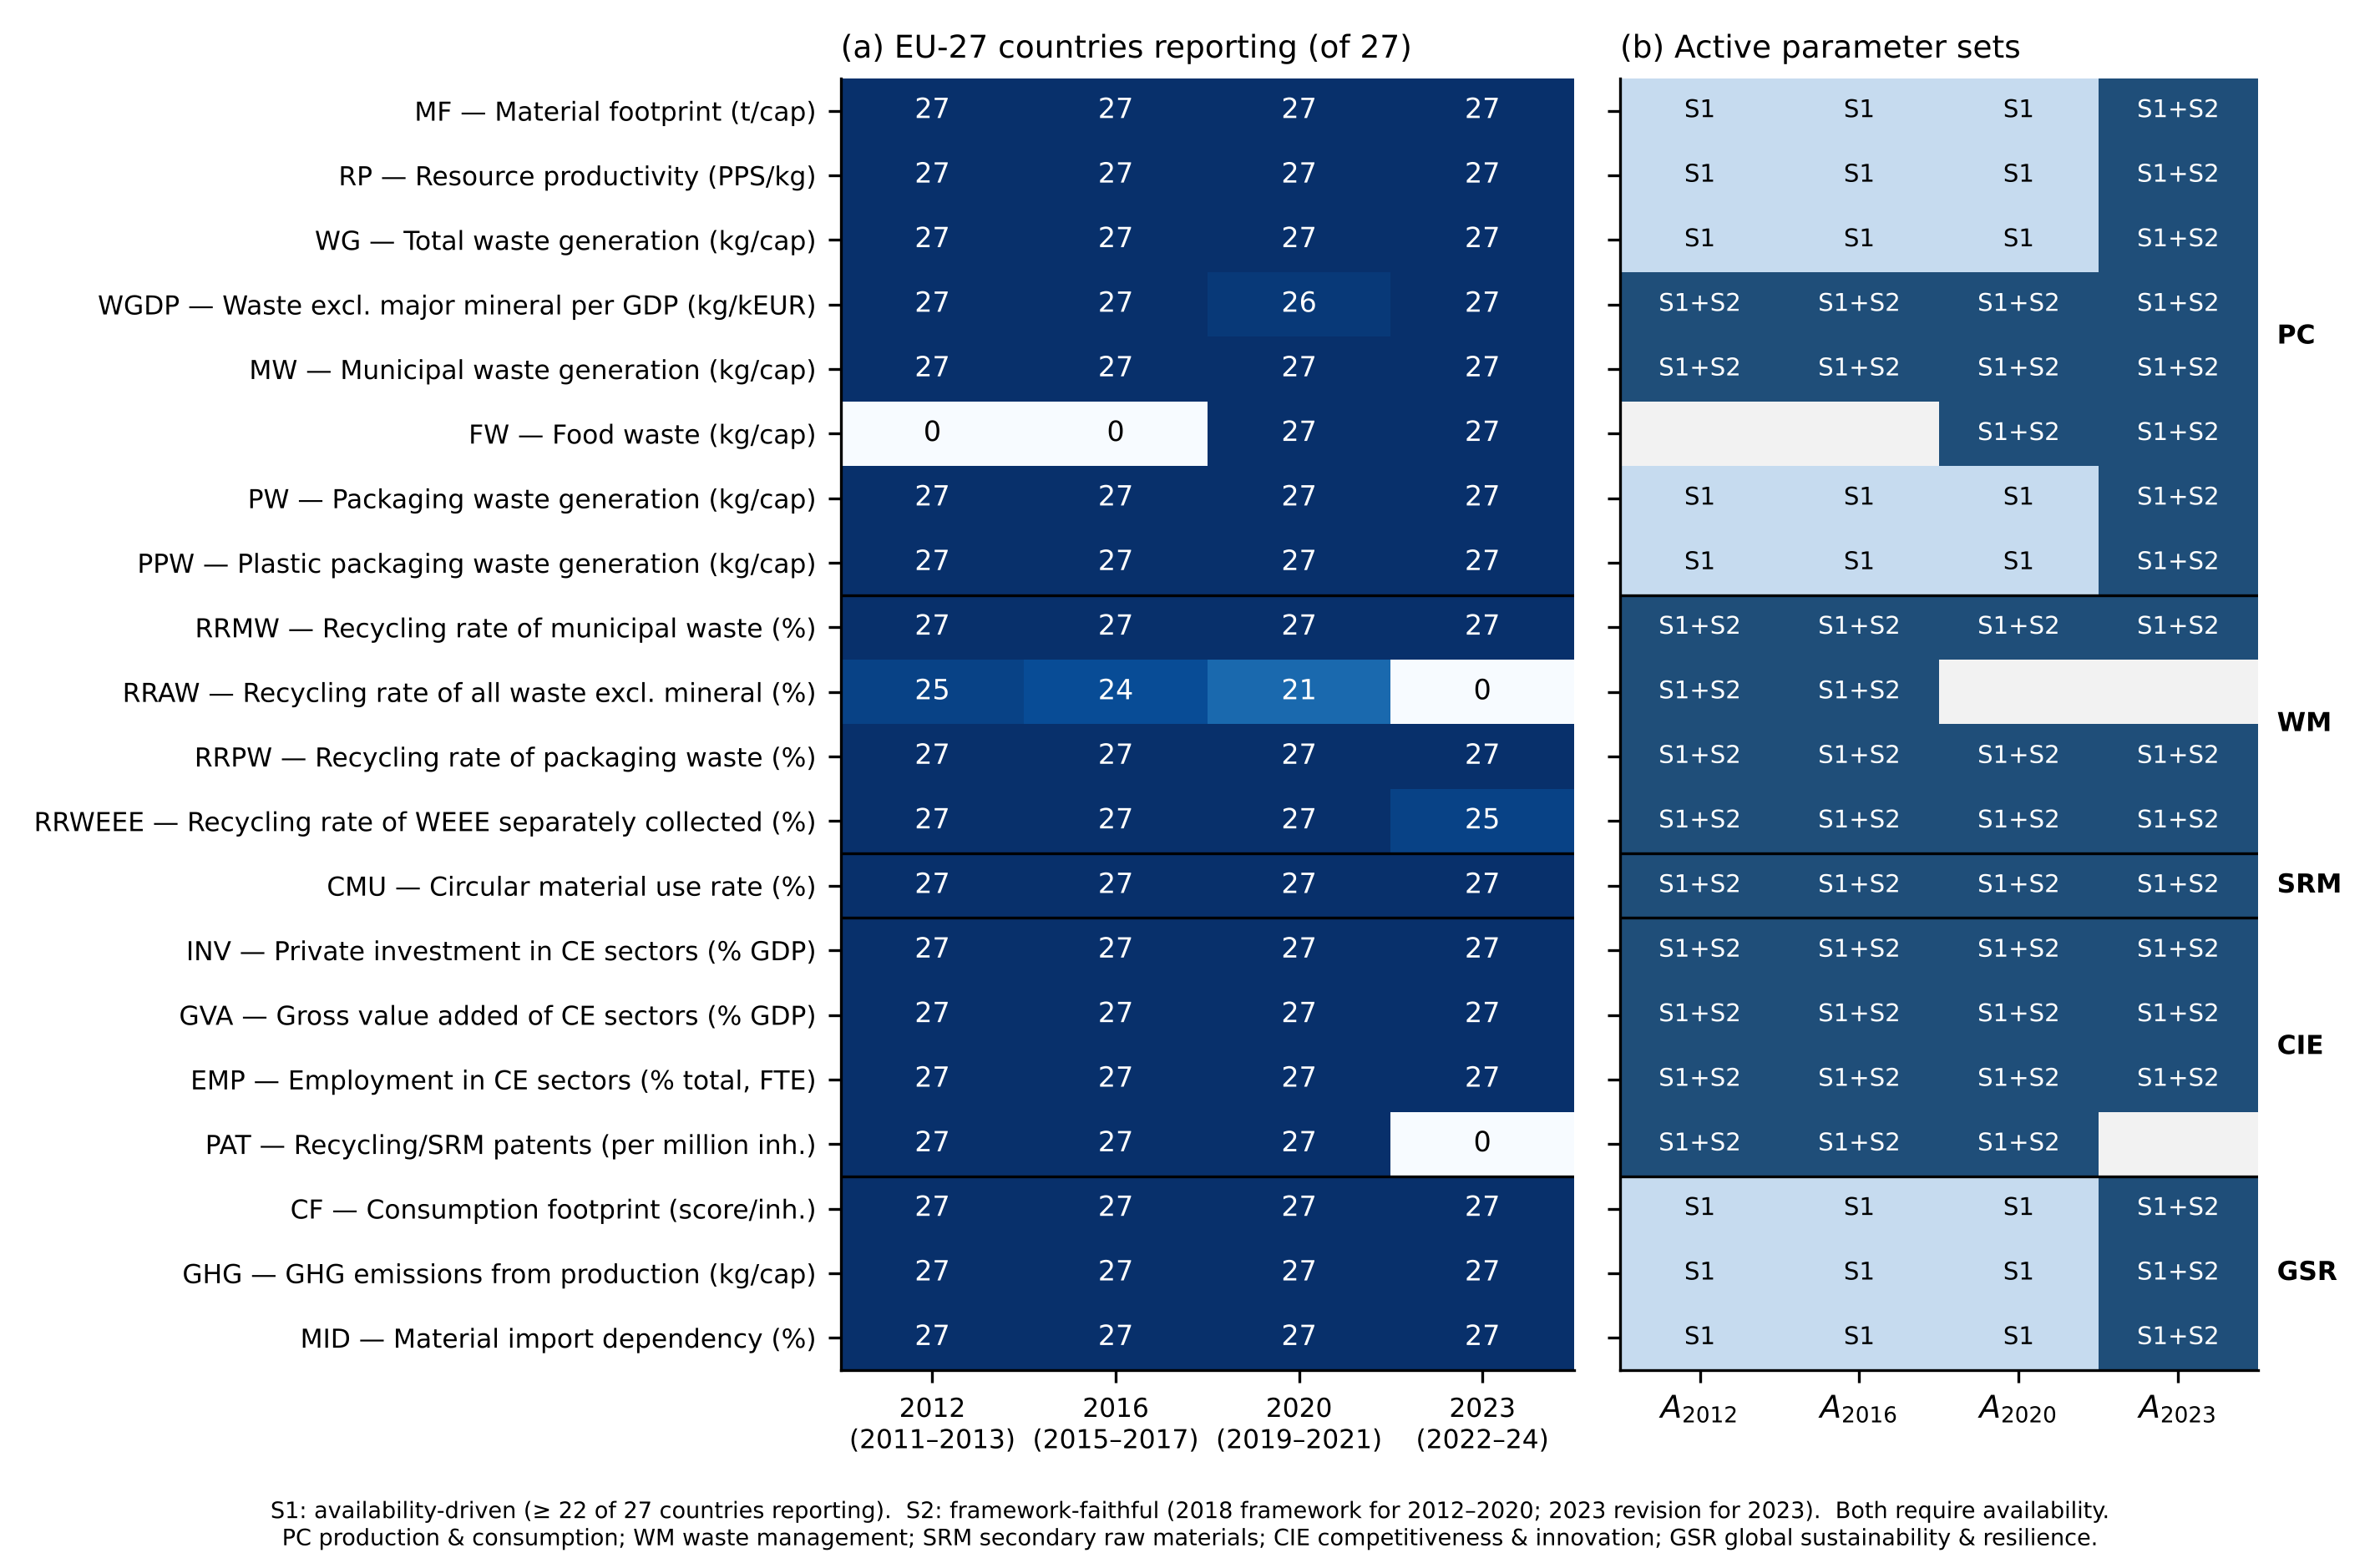
\includegraphics[width=\textwidth]{Figure_1.png}
\caption{(a) Number of EU-27 member states reporting each indicator in each window and (b) membership of the availability-driven (S1) and framework-faithful (S2) active parameter sets $A_t$. Food waste becomes observable only from the 2020 window; all-waste recycling and patents are discontinued before the 2023 window; the 2023 revision adds eight indicators to the framework-faithful set.}\label{fig:avail}\end{figure*}

\subsubsection{The active sets} Figure~\ref{fig:avail} and Table~\ref{tab:indicators} establish the structural facts. Food waste has no data before 2020; the recycling rate of all waste excluding major mineral waste is discontinued after 2020 and falls below the reporting threshold in the 2020 window; the patent series ends in 2021. Under the framework in force, the active set grows from eleven indicators in 2012--2020 to eighteen in 2023. The flagged share of observations rises from 8\,\% to 22\,\% across the windows, and mean confidence falls from 0.972 to 0.963.


\subsubsection{Scores and period rankings} Table~\ref{tab:dfss} and Fig.~\ref{fig:bump} report the DFSS results under Scenario~S2. The Netherlands leads the global ranking ($P=0.681$), followed by Belgium (0.617), Luxembourg (0.607), France, Italy, Austria, Germany and Estonia; Greece (0.337), Romania, Cyprus and Bulgaria close the ranking. The period rankings show the consequence of the 2023 revision directly: Luxembourg is first, third and third in the 2012, 2016 and 2020 windows and tenth in 2023; Denmark falls from fifteenth to twenty-third; Croatia rises from seventeenth to thirteenth, Slovakia from twelfth to eighth and Estonia from sixth to second in the same step.

\begin{figure}[pos=t]\centering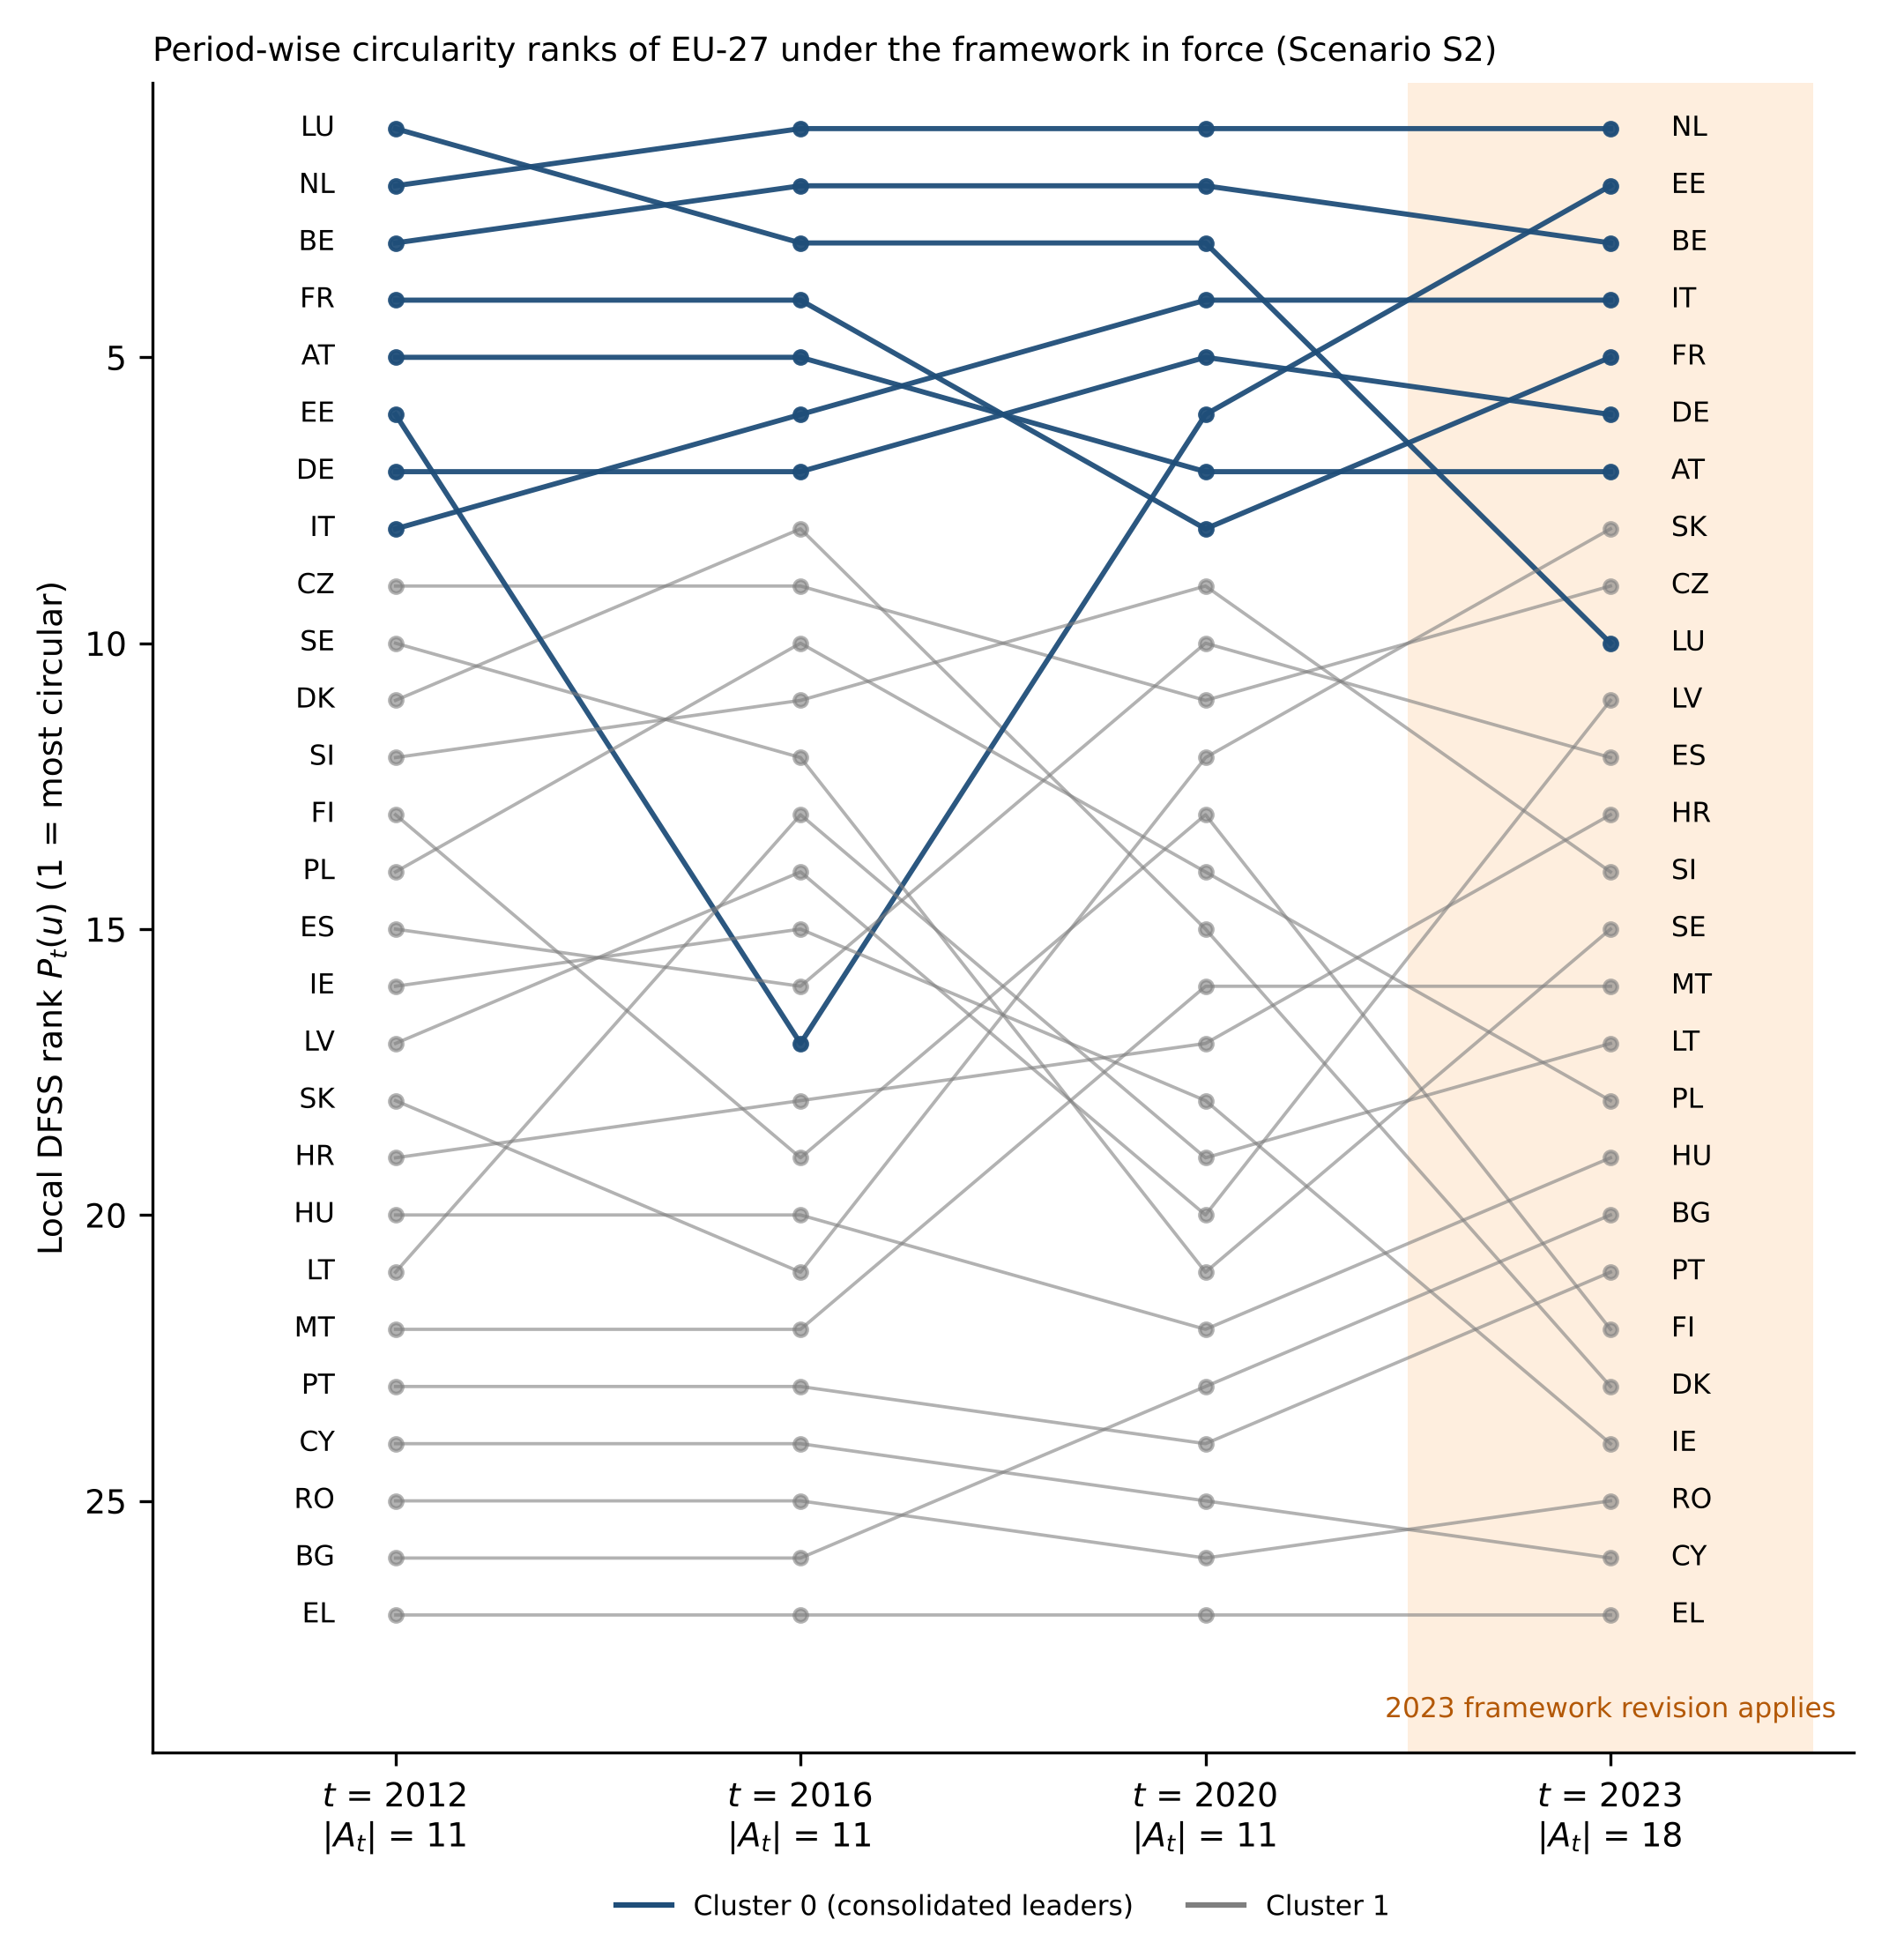
\includegraphics[width=\columnwidth]{Figure_2.png}
\caption{Period-wise DFSS ranks of EU-27 under the framework in force (Scenario S2). Dark lines: consolidated-leader cluster. The shaded column marks the window in which the 2023 revision applies.}\label{fig:bump}\end{figure}

\begin{table*}[pos=t]\centering\footnotesize
\caption{DFSS circularity scores of EU-27 under the framework in force (Scenario S2, dimension-balanced weights): local scores $P_t(u)$ with period rank in parentheses, global score $P(u)$, rank range across the 36 alternative specifications of the sensitivity grid (Fig.~S1), and trajectory cluster (0 = consolidated leaders). MS: member state (ISO 3166 code).}
\label{tab:dfss}
\begin{adjustbox}{max width=\linewidth}\begin{tabular}{@{}rlccccccc@{}}\toprule
Rank & MS & $P_{2012}$ & $P_{2016}$ & $P_{2020}$ & $P_{2023}$ & $P(u)$ & Range & Cluster \\ \midrule
1 & NL & 0.663 (2) & 0.689 (1) & 0.693 (1) & 0.681 (1) & 0.681 & 1--3 & 0 \\
2 & BE & 0.611 (3) & 0.615 (2) & 0.628 (2) & 0.612 (3) & 0.617 & 2--5 & 0 \\
3 & LU & 0.691 (1) & 0.608 (3) & 0.596 (3) & 0.534 (10) & 0.607 & 1--11 & 0 \\
4 & FR & 0.575 (4) & 0.587 (4) & 0.552 (8) & 0.586 (5) & 0.575 & 3--12 & 0 \\
5 & IT & 0.508 (8) & 0.547 (6) & 0.594 (4) & 0.602 (4) & 0.563 & 3--9 & 0 \\
6 & AT & 0.542 (5) & 0.562 (5) & 0.570 (7) & 0.568 (7) & 0.561 & 3--7 & 0 \\
7 & DE & 0.515 (7) & 0.512 (7) & 0.577 (5) & 0.583 (6) & 0.547 & 4--8 & 0 \\
8 & EE & 0.516 (6) & 0.443 (17) & 0.570 (6) & 0.623 (2) & 0.538 & 5--20 & 0 \\
9 & CZ & 0.482 (9) & 0.489 (9) & 0.524 (11) & 0.545 (9) & 0.510 & 3--12 & 1 \\
10 & SI & 0.454 (12) & 0.477 (11) & 0.536 (9) & 0.523 (14) & 0.498 & 9--18 & 1 \\
11 & ES & 0.447 (15) & 0.450 (16) & 0.528 (10) & 0.529 (12) & 0.488 & 9--19 & 1 \\
12 & SE & 0.481 (10) & 0.466 (12) & 0.458 (21) & 0.509 (15) & 0.478 & 10--19 & 1 \\
13 & SK & 0.413 (18) & 0.421 (21) & 0.502 (12) & 0.562 (8) & 0.474 & 6--21 & 1 \\
14 & DK & 0.470 (11) & 0.508 (8) & 0.471 (15) & 0.449 (23) & 0.474 & 8--24 & 1 \\
15 & PL & 0.450 (14) & 0.482 (10) & 0.478 (14) & 0.486 (18) & 0.474 & 13--20 & 1 \\
16 & LV & 0.422 (17) & 0.461 (14) & 0.463 (20) & 0.530 (11) & 0.469 & 8--16 & 1 \\
17 & HR & 0.401 (19) & 0.443 (18) & 0.467 (17) & 0.528 (13) & 0.460 & 8--24 & 1 \\
18 & FI & 0.451 (13) & 0.427 (19) & 0.487 (13) & 0.450 (22) & 0.454 & 2--23 & 1 \\
19 & LT & 0.393 (21) & 0.461 (13) & 0.464 (19) & 0.492 (17) & 0.452 & 12--21 & 1 \\
20 & IE & 0.429 (16) & 0.453 (15) & 0.466 (18) & 0.440 (24) & 0.447 & 9--25 & 1 \\
21 & HU & 0.396 (20) & 0.424 (20) & 0.450 (22) & 0.484 (19) & 0.439 & 17--23 & 1 \\
22 & MT & 0.390 (22) & 0.393 (22) & 0.470 (16) & 0.499 (16) & 0.438 & 16--25 & 1 \\
23 & PT & 0.384 (23) & 0.392 (23) & 0.403 (24) & 0.470 (21) & 0.412 & 20--23 & 1 \\
24 & BG & 0.317 (26) & 0.364 (26) & 0.421 (23) & 0.470 (20) & 0.393 & 19--26 & 1 \\
25 & CY & 0.382 (24) & 0.388 (24) & 0.374 (25) & 0.420 (26) & 0.391 & 21--26 & 1 \\
26 & RO & 0.373 (25) & 0.372 (25) & 0.354 (26) & 0.432 (25) & 0.383 & 21--26 & 1 \\
27 & EL & 0.288 (27) & 0.322 (27) & 0.341 (27) & 0.397 (27) & 0.337 & 27--27 & 1 \\
\bottomrule\end{tabular}\end{adjustbox}\end{table*}


\subsubsection{Decomposing the 2023 break} Equation~\eqref{eq:decomp} separates the 2020$\to$2023 change into value and structural effects (Table~\ref{tab:decomp}, Fig.~\ref{fig:decomp}). Across the twenty-seven member states, 65\,\% of the total absolute change in local scores is structural, that is, attributable to the eight indicators entering $A_{2023}$ rather than to performance, and the structural component exceeds the value component in twenty of them (three of these, Spain, Italy and France, only marginally). The largest negative structural effects fall on Luxembourg ($-0.059$, against a value effect of $-0.003$; period rank 3$\to$10), Ireland ($-0.039$; 18$\to$24), Estonia ($-0.037$, more than offset by a value effect of $+0.089$; 6$\to$2), the Netherlands ($-0.034$, which retains first place) and Denmark ($-0.020$; 15$\to$23); the largest positive ones on Romania ($+0.122$), Greece ($+0.072$), Bulgaria ($+0.071$), Croatia ($+0.061$, with a value effect of $-0.000$; 17$\to$13), Portugal ($+0.058$) and Cyprus ($+0.049$). The entering indicators are consumption-side footprints and import dependency, which favour low-consumption economies; the revision therefore re-weighted the concept of circularity from waste-management and circular-sector performance toward consumption footprints and resilience. Under dimension-balanced weights the entering indicators share the weight of their dimensions rather than adding to it, so these effects are smaller than under equal indicator weights (by about a quarter in aggregate and by half for Luxembourg); the share of structural change is 65\,\% under both weightings. The counterfactual set omits the patent indicator, discontinued in 2021, so its exit is carried in the value term (Eq.~\eqref{eq:decomp}). By contrast the 2016$\to$2020 activation of food waste has a mean absolute structural effect of only 0.017.

\begin{figure}[pos=t]\centering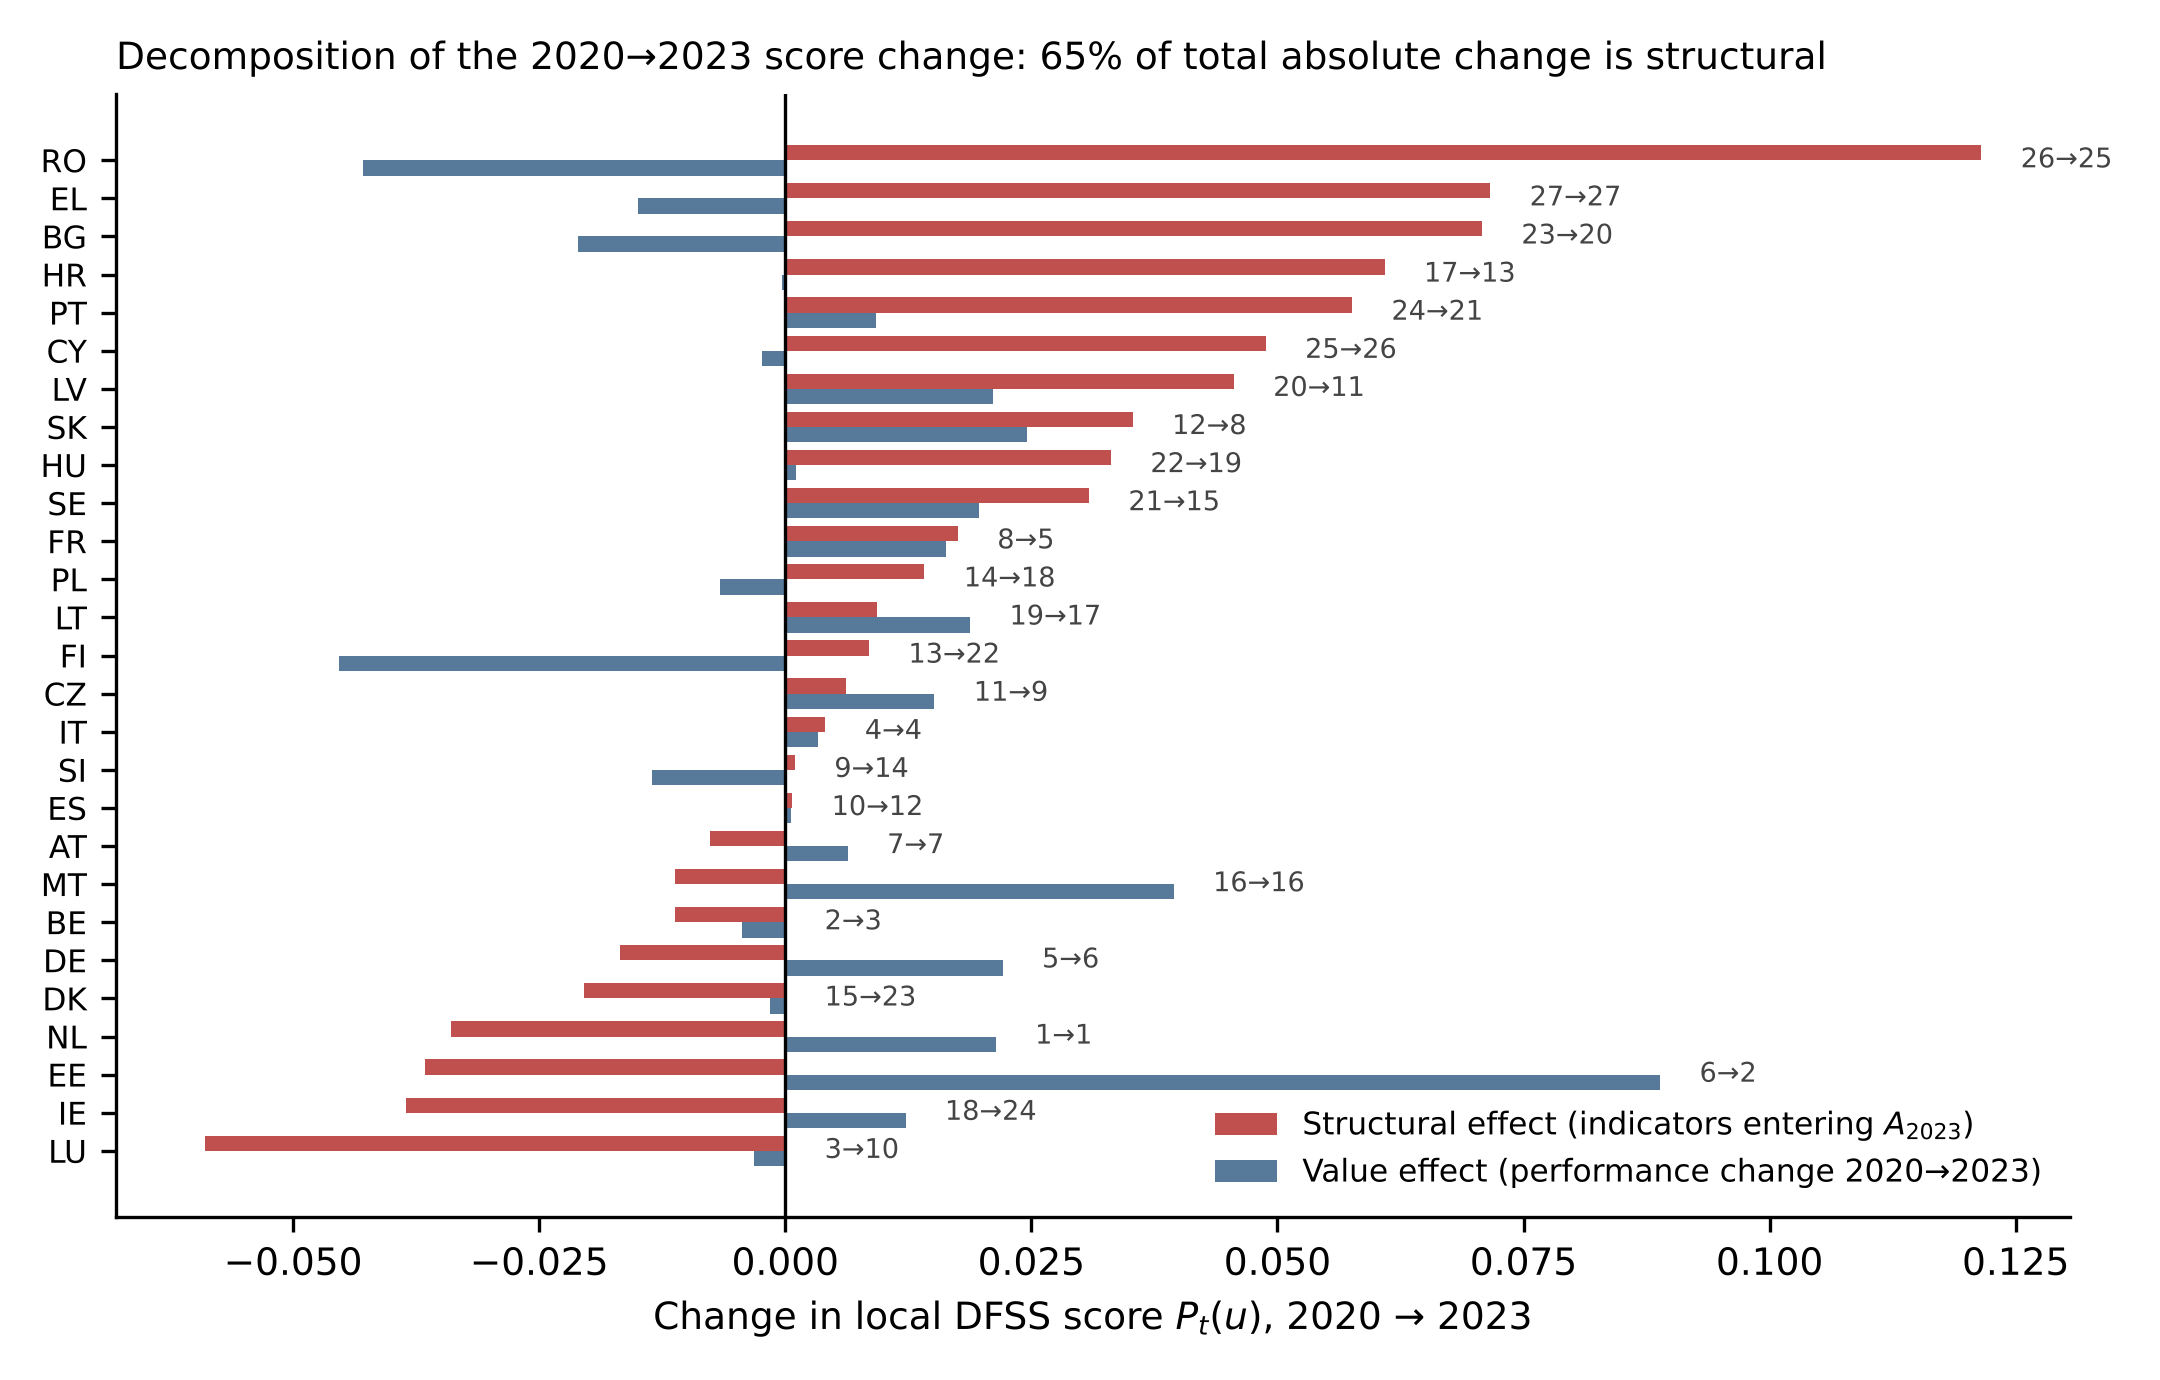
\includegraphics[width=\columnwidth]{Figure_3.png}
\caption{Decomposition of the 2020$\to$2023 change in local DFSS score into a structural effect (indicators entering $A_{2023}$) and a value effect (performance change). Labels give period rank before and after.}\label{fig:decomp}\end{figure}

\begin{table*}[pos=t]\centering\footnotesize
\caption{Decomposition of the change in local score between the 2020 and 2023 windows into a value effect (performance change evaluated on the counterfactual set $A_{2020}\cap\{e:\ e \text{ observed in } 2023\}$, which omits PAT, discontinued in 2021) and a structural effect (indicators entering $A_{2023}$: MF, RP, WG, PW, PPW, CF, GHG, MID). Seven largest negative and positive structural effects; rank$_{cf}$ is the 2023 rank that would have obtained under the counterfactual set. MS: member state. Across all 27 member states, 65\,\% of total absolute change is structural.}
\label{tab:decomp}
\begin{adjustbox}{max width=\linewidth}\begin{tabular}{@{}lccrrccc@{}}\toprule
MS & $P_{2020}$ & $P_{2023}$ & Value & Structural & rank$_{2020}$ & rank$_{cf}$ & rank$_{2023}$ \\ \midrule
LU & 0.596 & 0.534 & -0.003 & -0.059 & 3 & 6 & 10 \\
IE & 0.466 & 0.440 & +0.012 & -0.039 & 18 & 16 & 24 \\
EE & 0.570 & 0.623 & +0.089 & -0.037 & 6 & 2 & 2 \\
NL & 0.693 & 0.681 & +0.021 & -0.034 & 1 & 1 & 1 \\
DK & 0.471 & 0.449 & -0.002 & -0.020 & 15 & 19 & 23 \\
DE & 0.577 & 0.583 & +0.022 & -0.017 & 5 & 4 & 6 \\
BE & 0.628 & 0.612 & -0.004 & -0.011 & 2 & 3 & 3 \\
LV & 0.463 & 0.530 & +0.021 & +0.046 & 20 & 14 & 11 \\
CY & 0.374 & 0.420 & -0.002 & +0.049 & 25 & 25 & 26 \\
PT & 0.403 & 0.470 & +0.009 & +0.058 & 24 & 23 & 21 \\
HR & 0.467 & 0.528 & -0.000 & +0.061 & 17 & 20 & 13 \\
BG & 0.421 & 0.470 & -0.021 & +0.071 & 23 & 24 & 20 \\
EL & 0.341 & 0.397 & -0.015 & +0.072 & 27 & 26 & 27 \\
RO & 0.354 & 0.432 & -0.043 & +0.122 & 26 & 27 & 25 \\
\bottomrule\end{tabular}\end{adjustbox}\end{table*}


\subsubsection{Why not a composite index} Table~\ref{tab:baselines} and Fig.~\ref{fig:baselines} answer the question empirically. The pooled composite B1 agrees closely with the DFSS global ranking ($\tau_b=0.977$, maximum shift two positions) because, with equal period weights and four windows, the cardinality bias is modest at the global level; it is the two remedies for a changing indicator set that fail, and they fail in opposite directions. Back-imputing the full twenty-indicator panel to 2012 (B2) yields $\tau_b=0.709$ with twelve member states shifting three or more positions and a maximum of nine: Croatia, Romania and Latvia are promoted by nine, seven and six positions and Denmark and Estonia demoted by nine and six, on the strength of footprint indicators applied to years for which they were never part of the framework. Restricting to the nine indicators active in every window (B3) preserves the global ordering better ($\tau_b=0.858$) but cannot see the revision: its agreement with the DFSS period ranking declines monotonically from $\tau_b=0.93$ in 2012 to 0.88, 0.82 and 0.71 in 2023, where eleven member states differ by three or more positions. Fuzzy TOPSIS per window (B4) agrees at $\tau_b=0.79$ globally and between 0.74 and 0.82 per window, the difference arising from its distance-to-ideal geometry rather than from the criteria set. In the availability-driven scenario S1, where $|A_t|$ hardly varies, the composite baselines converge on the DFSS ($\tau_b\ge0.90$; TOPSIS 0.66), which confirms that the divergence in S2 is produced by the structural change and not by the method.

\begin{figure}[pos=t]\centering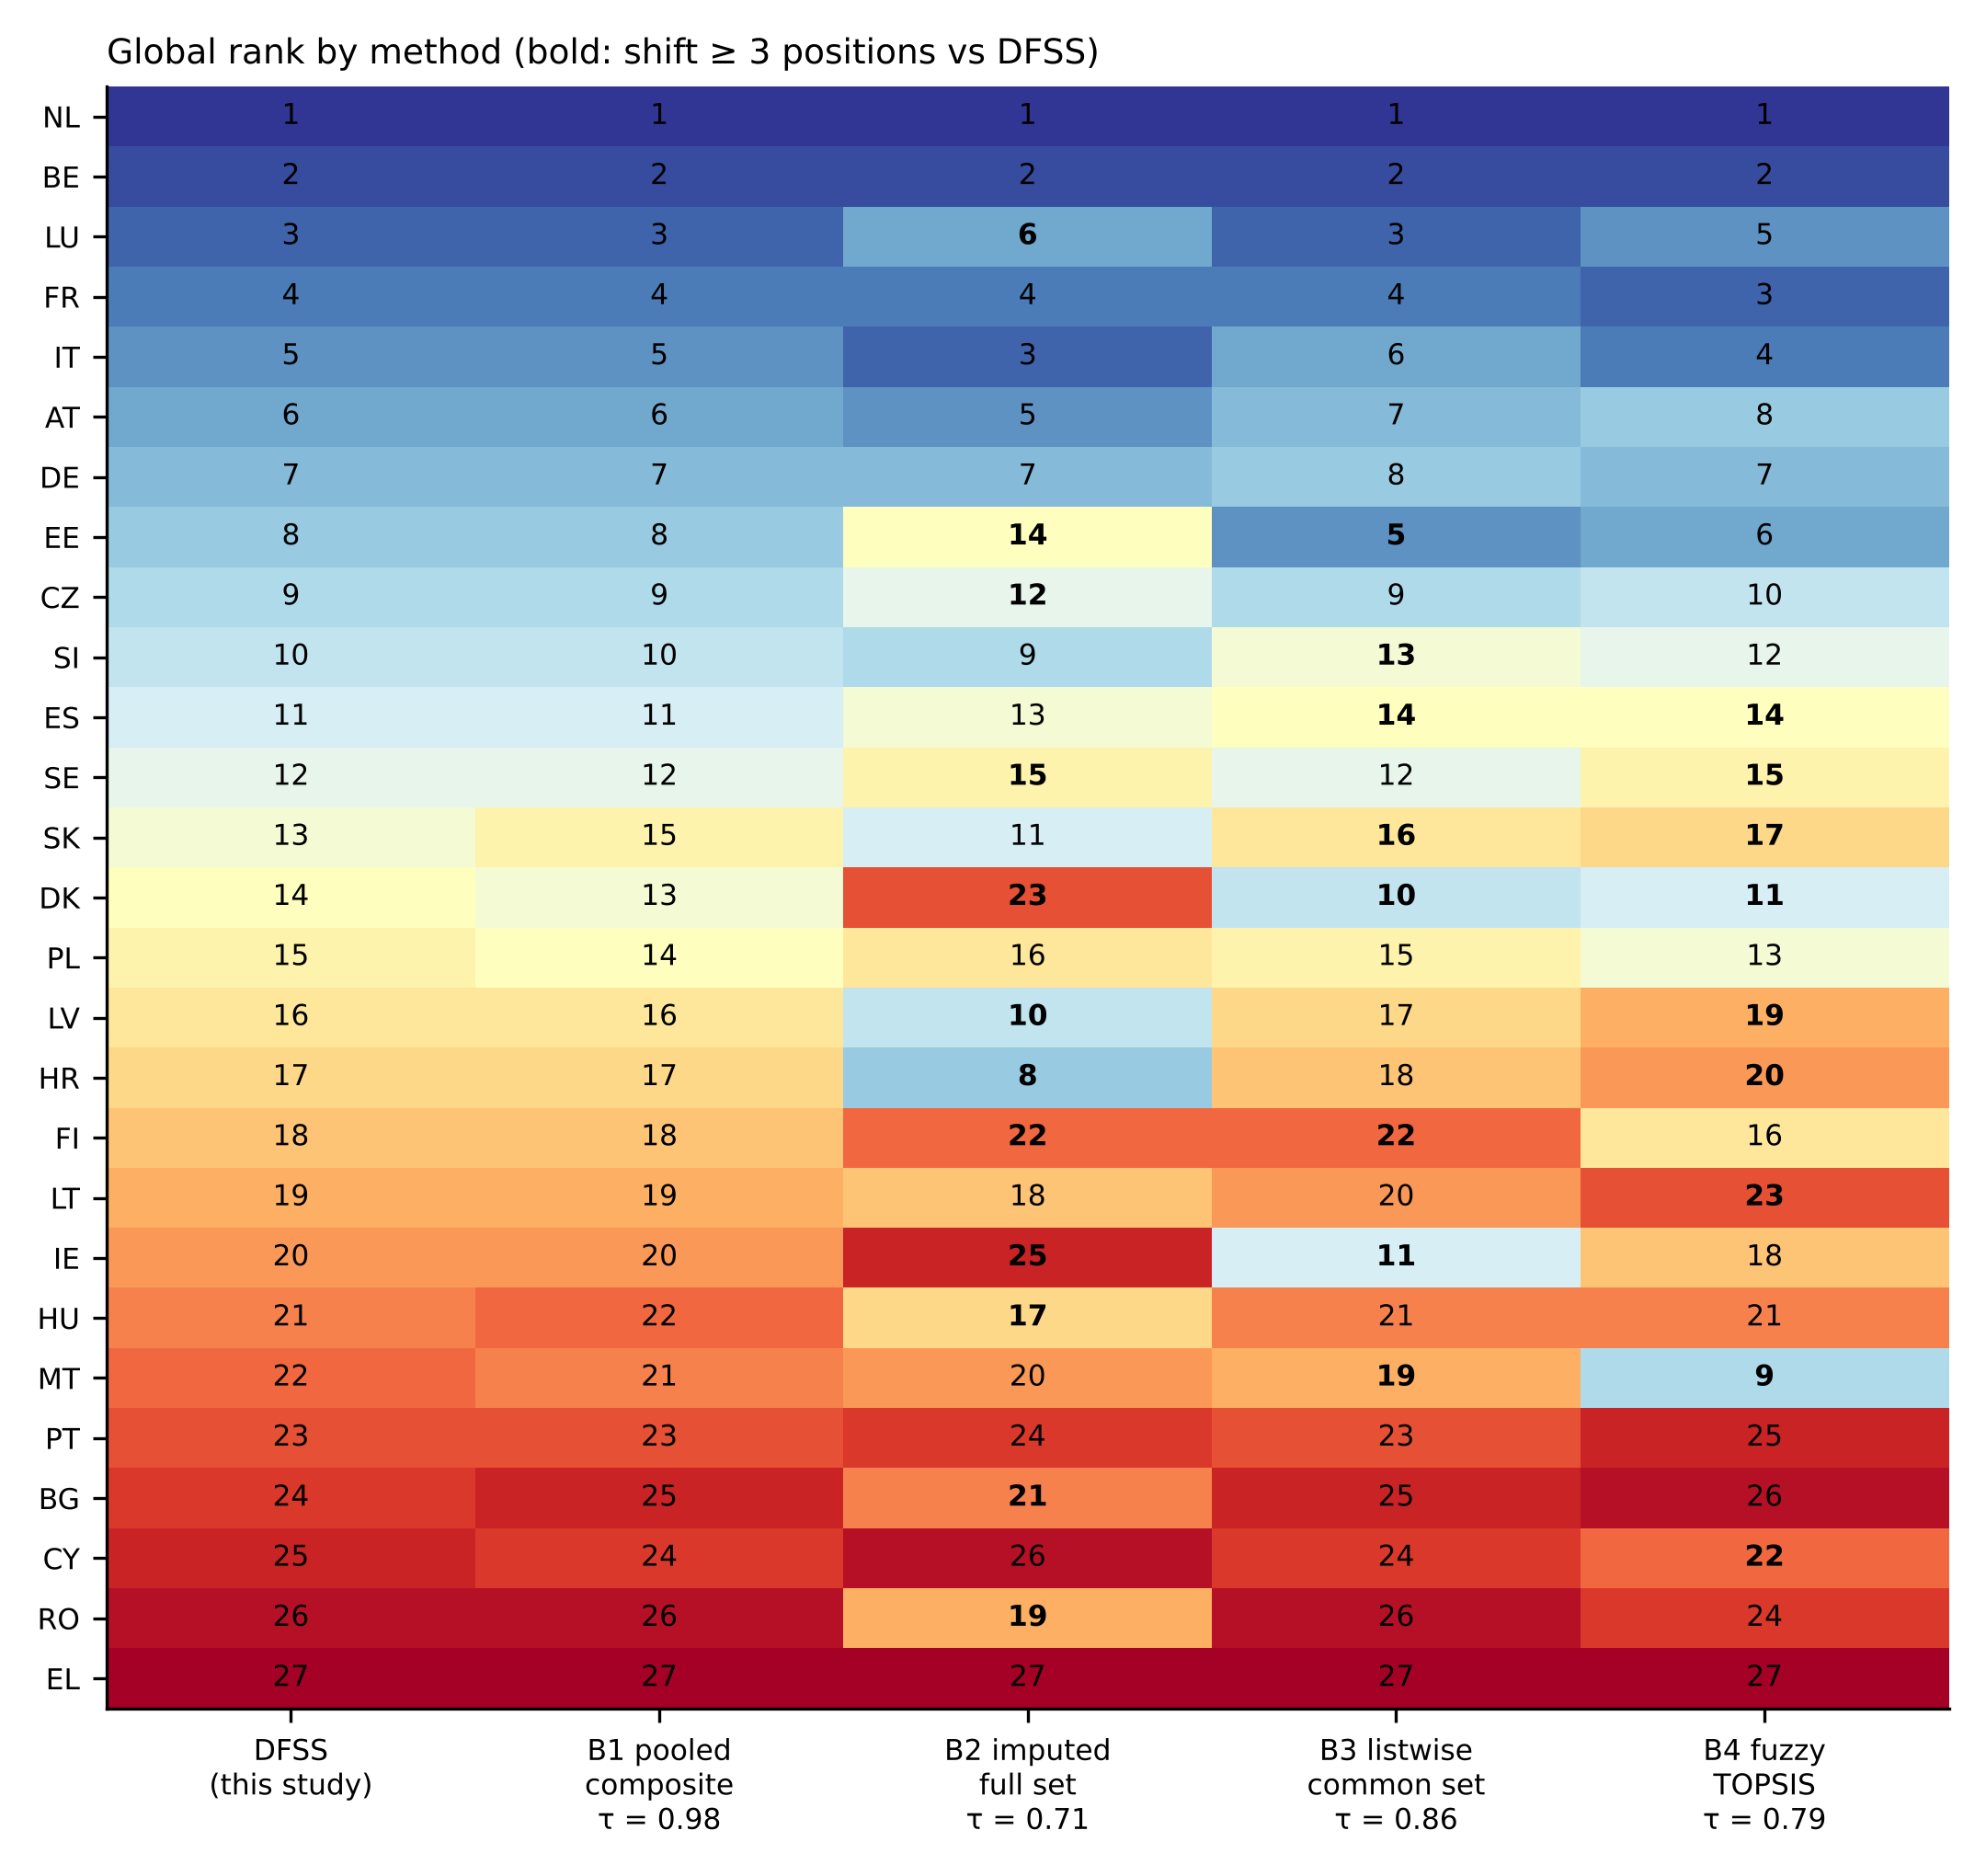
\includegraphics[width=\columnwidth]{Figure_4.png}
\caption{Global rank of each member state by method (Scenario S2). Bold entries shift by three or more positions relative to the DFSS.}\label{fig:baselines}\end{figure}

\begin{table*}[pos=t]\centering\footnotesize
\caption{Agreement between the DFSS global ranking and conventional aggregation baselines. Left block: Scenario S2 (framework-faithful); right block: Scenario S1 (availability-driven). Lower block: agreement per period, with the window years as column headers.}
\label{tab:baselines}
\begin{adjustbox}{max width=\linewidth}\begin{tabular}{@{}lcccccc@{}}\toprule
 & \multicolumn{4}{c}{S2} & \multicolumn{2}{c}{S1} \\ \cmidrule(lr){2-5}\cmidrule(lr){6-7}
Baseline & $\tau_b$ & $r_s$ & Max shift & $n(|\Delta|\ge3)$ & $\tau_b$ & Max shift \\ \midrule
B1 Pooled composite (all $(t,e)$ pairs) & 0.977 & 0.997 & 2 & 0 & 0.972 & 2 \\
B2 Full-set composite with cross-period imputation & 0.709 & 0.879 & 9 & 12 & 0.915 & 5 \\
B3 Listwise composite (9 common indicators) & 0.858 & 0.949 & 9 & 8 & 0.909 & 7 \\
B4 Fuzzy TOPSIS per period & 0.789 & 0.909 & 13 & 9 & 0.664 & 11 \\
\midrule \multicolumn{7}{l}{\emph{Per-period agreement with the DFSS local ranking (S2), Kendall $\tau_b$}} \\
 & 2012 & 2016 & 2020 & 2023 & & \\ \cmidrule(lr){2-5}
B3 Listwise & 0.93 & 0.88 & 0.82 & 0.71 & & \\
B4 Fuzzy TOPSIS & 0.77 & 0.78 & 0.82 & 0.74 & & \\
\bottomrule\end{tabular}\end{adjustbox}\end{table*}


\subsubsection{Trajectory archetypes} Silhouette selects $k=2$ (0.45), with bootstrap Jaccard stability 0.85 (Fig.~\ref{fig:clusters}). Cluster~0, the consolidated leaders, comprises Austria, Belgium, Germany, Estonia, France, Italy, Luxembourg and the Netherlands; cluster~1 the remaining nineteen. Agreement with Ward clustering is moderate (adjusted Rand 0.57), so the two-cluster solution is presented as a coarse typology and refined by wave timing in Section~\ref{sec:resGap}.

\begin{figure}[pos=t]\centering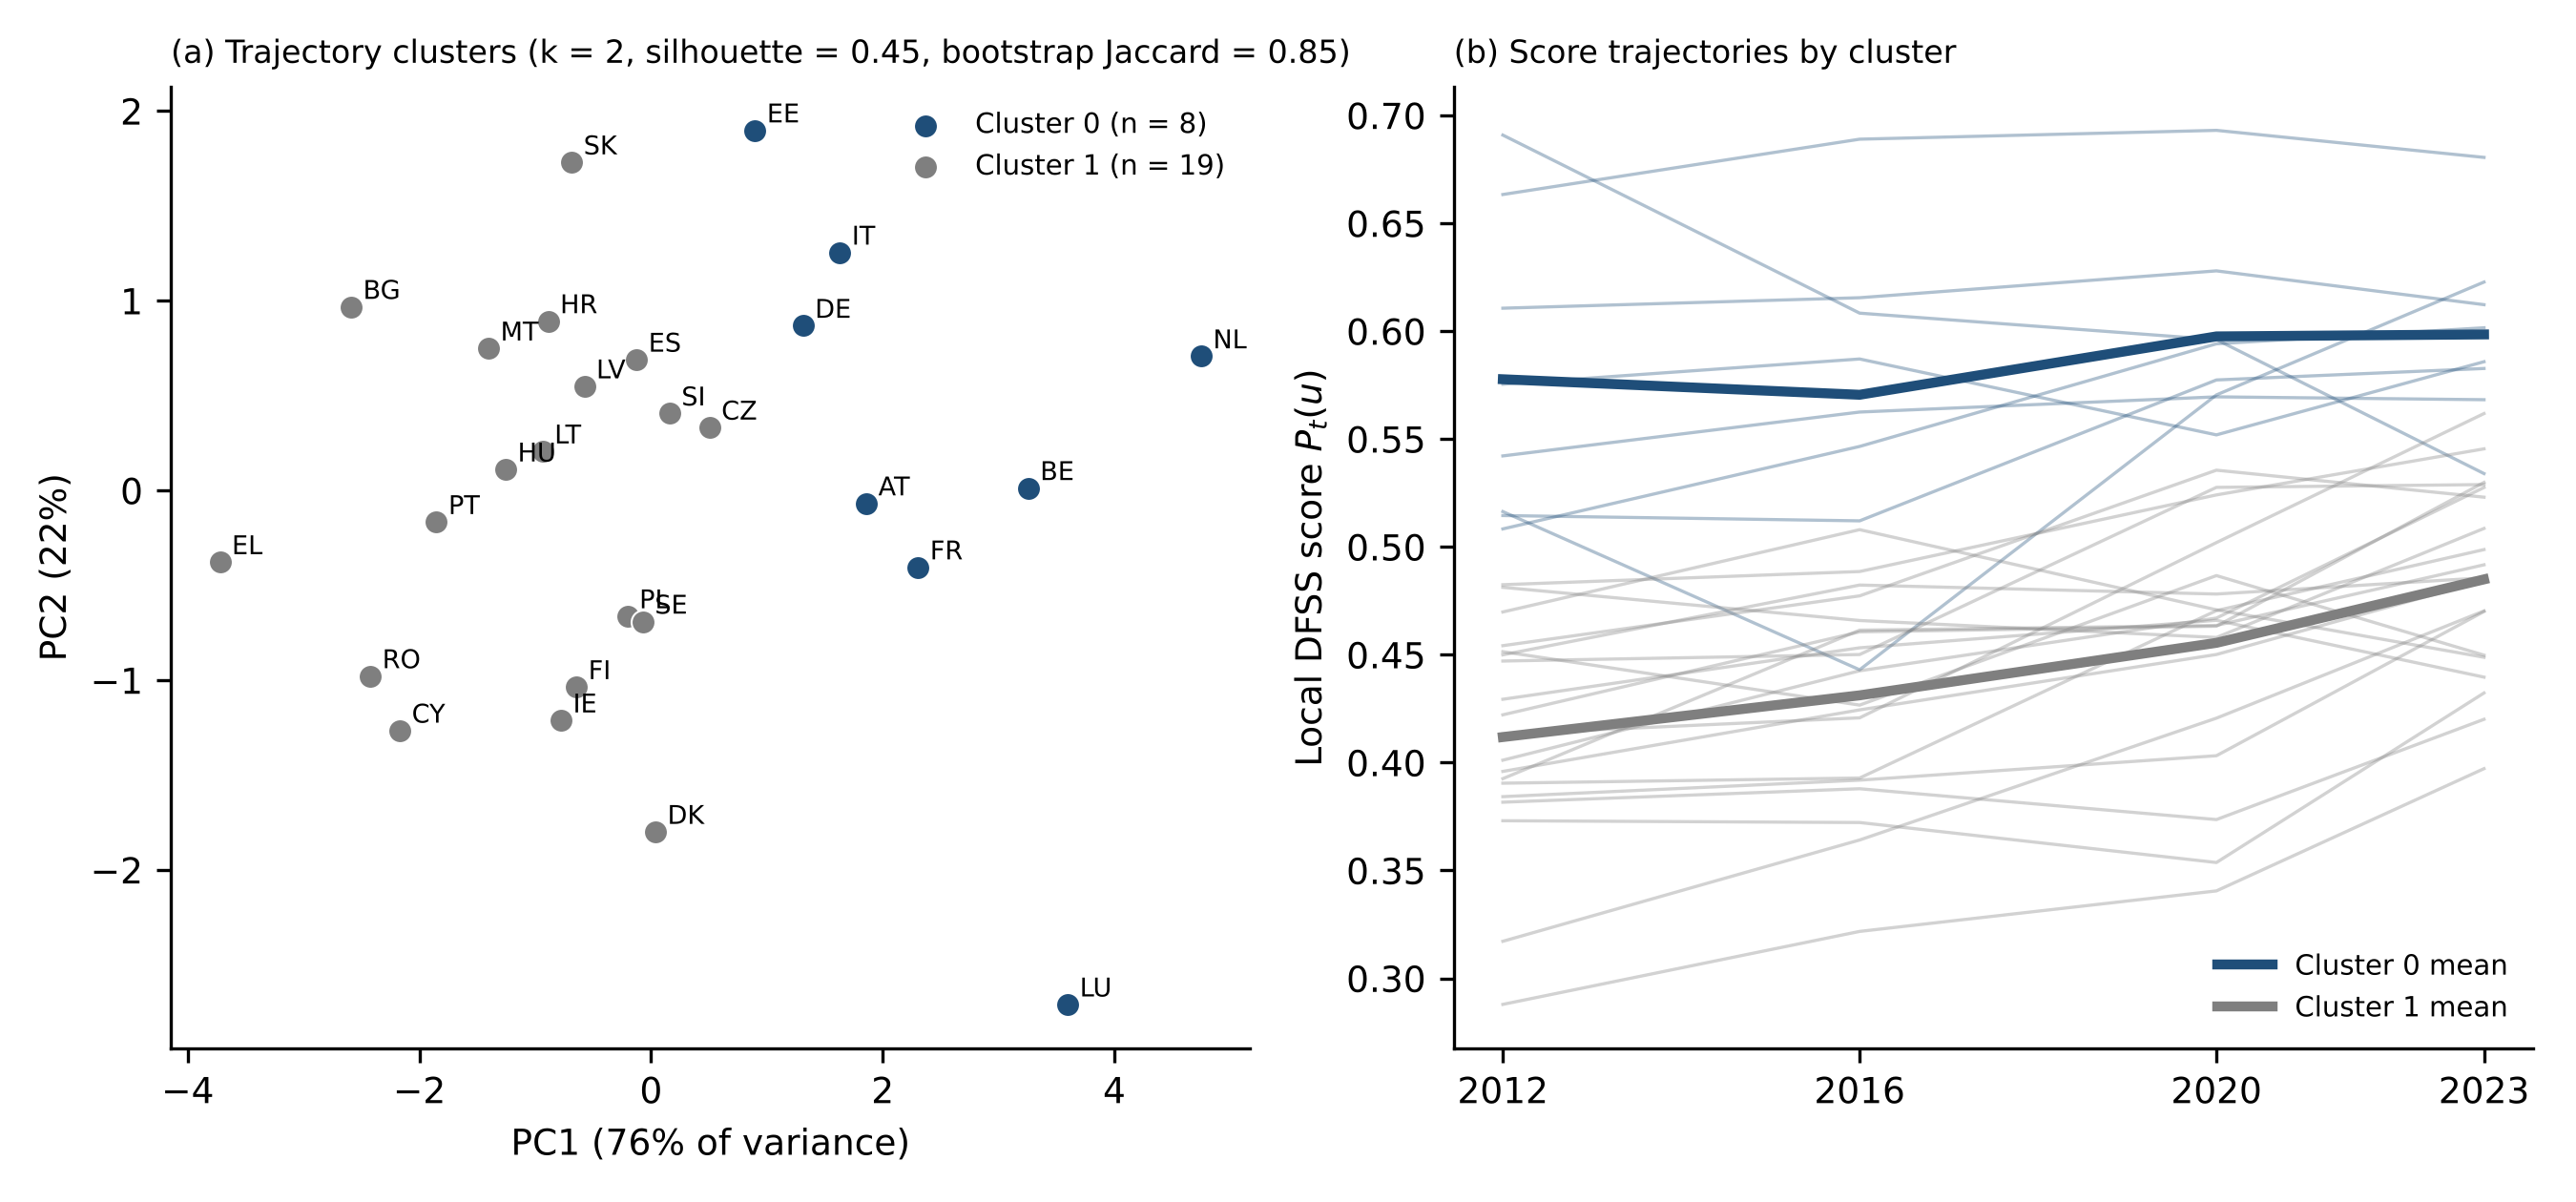
\includegraphics[width=\columnwidth]{Figure_5.png}
\caption{(a) Trajectory clusters in the first two principal components of $(P_{2012},\dots,P_{2023},\text{slope})$; (b) score trajectories by cluster.}\label{fig:clusters}\end{figure}

\subsubsection{Sensitivity} Across 36 alternative specifications (two normalisations, three weightings, confidence on or off and three period weightings, less the primary, plus Scenario~S1), the median Kendall $\tau_b$ with the primary specification is 0.75 and the minimum 0.61 (Supplementary Fig.~S1). The dimension-balanced weighting is the most stable across the other choices (mean $\tau_b=0.89$ versus 0.73 for equal-per-indicator and 0.70 for entropy weights). Switching confidence weighting off yields a ranking that agrees with the primary specification at $\tau_b=0.98$: it is necessary for honest bookkeeping but nearly immaterial for the ordering; replacing reference by min--max normalisation gives $\tau_b=0.84$. The Netherlands ranks between first and third in every specification, Belgium between second and fifth, and Greece is always last; volatility concentrates in Finland (2--23), Croatia (8--24), Denmark (8--24), Ireland (9--25), Estonia (5--20) and Slovakia (6--21), member states whose profiles are polarised across dimensions. Varying the reporting threshold from 18 to 26 within Scenario~S2 (where the threshold can only remove indicators from $A_t$) leaves the ranking unchanged except at the extreme ($\tau_b=0.97$ at 26). Scenarios S1 and S2 agree at $\tau_b=0.75$; the largest differences (Denmark, Croatia, Bulgaria, Finland, Ireland, Romania) are precisely the countries most affected by the footprint indicators.


\subsection{Layer B: the PV waste wave}\label{sec:resB}

\subsubsection{Calibration and validation} Figure~\ref{fig:valid} compares modelled arisings with PV panels separately collected in 2016--2024. The calibrated early-loss share is $\pi=0.18$ on 71 country-years. For Germany, the member state with the largest fleet, collection rose from \SI{2.0}{kt} in 2016 to 13.4, 15.4, 16.1 and \SI{16.4}{kt} in 2019--2022, against central-scenario arisings of 13.6, 17.0, 21.2 and \SI{26.3}{kt}: the central scenario tracks the observed level within 11\,\% in 2019--2020 and over-predicts by 32\,\% in 2021 and 60\,\% in 2022, while the early-loss scenario over-predicts by a factor of four and the regular-loss scenario under-predicts by half in 2019--2020. The widening gap after 2020 coincides with the change to open-scope reporting and with arisings accelerating ahead of collection, and illustrates the point made by \citet{kastanaki2026}: judged against collection statistics, the regular-loss baseline is too low in the years for which the data are most complete. Country-specific fits on three or more qualifying years give $\pi=0.00$ for Spain, 0.03 for Czechia, 0.05 for Germany, 0.10 for Belgium, 0.11 for Italy, 0.14 for the Netherlands, 0.16 for Portugal, 0.28 for France and 0.89 for Poland, whose reported series is short and volatile; the pooled value of 0.18 therefore sits inside the range of the large fleets, which cluster between regular loss and the pooled value. Italy's whole-period fit is close to the pooled value, but its most recent years are the exception that proves the model's reading: collection jumped from \SI{6.5}{kt} in 2021 to 21.9 and \SI{30.0}{kt} in 2022--2023, approaching the early-loss envelope (31.7 and \SI{35.7}{kt}); this coincides with the revamping of Conto Energia plants, in which functioning modules are replaced during repowering, a retirement mechanism that the early-loss curve captures and the regular-loss curve cannot. Germany's reported collection fell to \SI{9.3}{kt} in 2024, a provisional figure, and the gap between the central scenario and reported collection widens in 2023--2024 in several states as arisings accelerate ahead of collection. The mass assumption is validated independently: across 107 country-years for which Eurostat reports PV modules put on the market in tonnes, the ratio of reported tonnage to capacity additions times the vintage mass factor has a median of 0.97 (interquartile range 0.72--1.30).

\begin{figure}[pos=t]\centering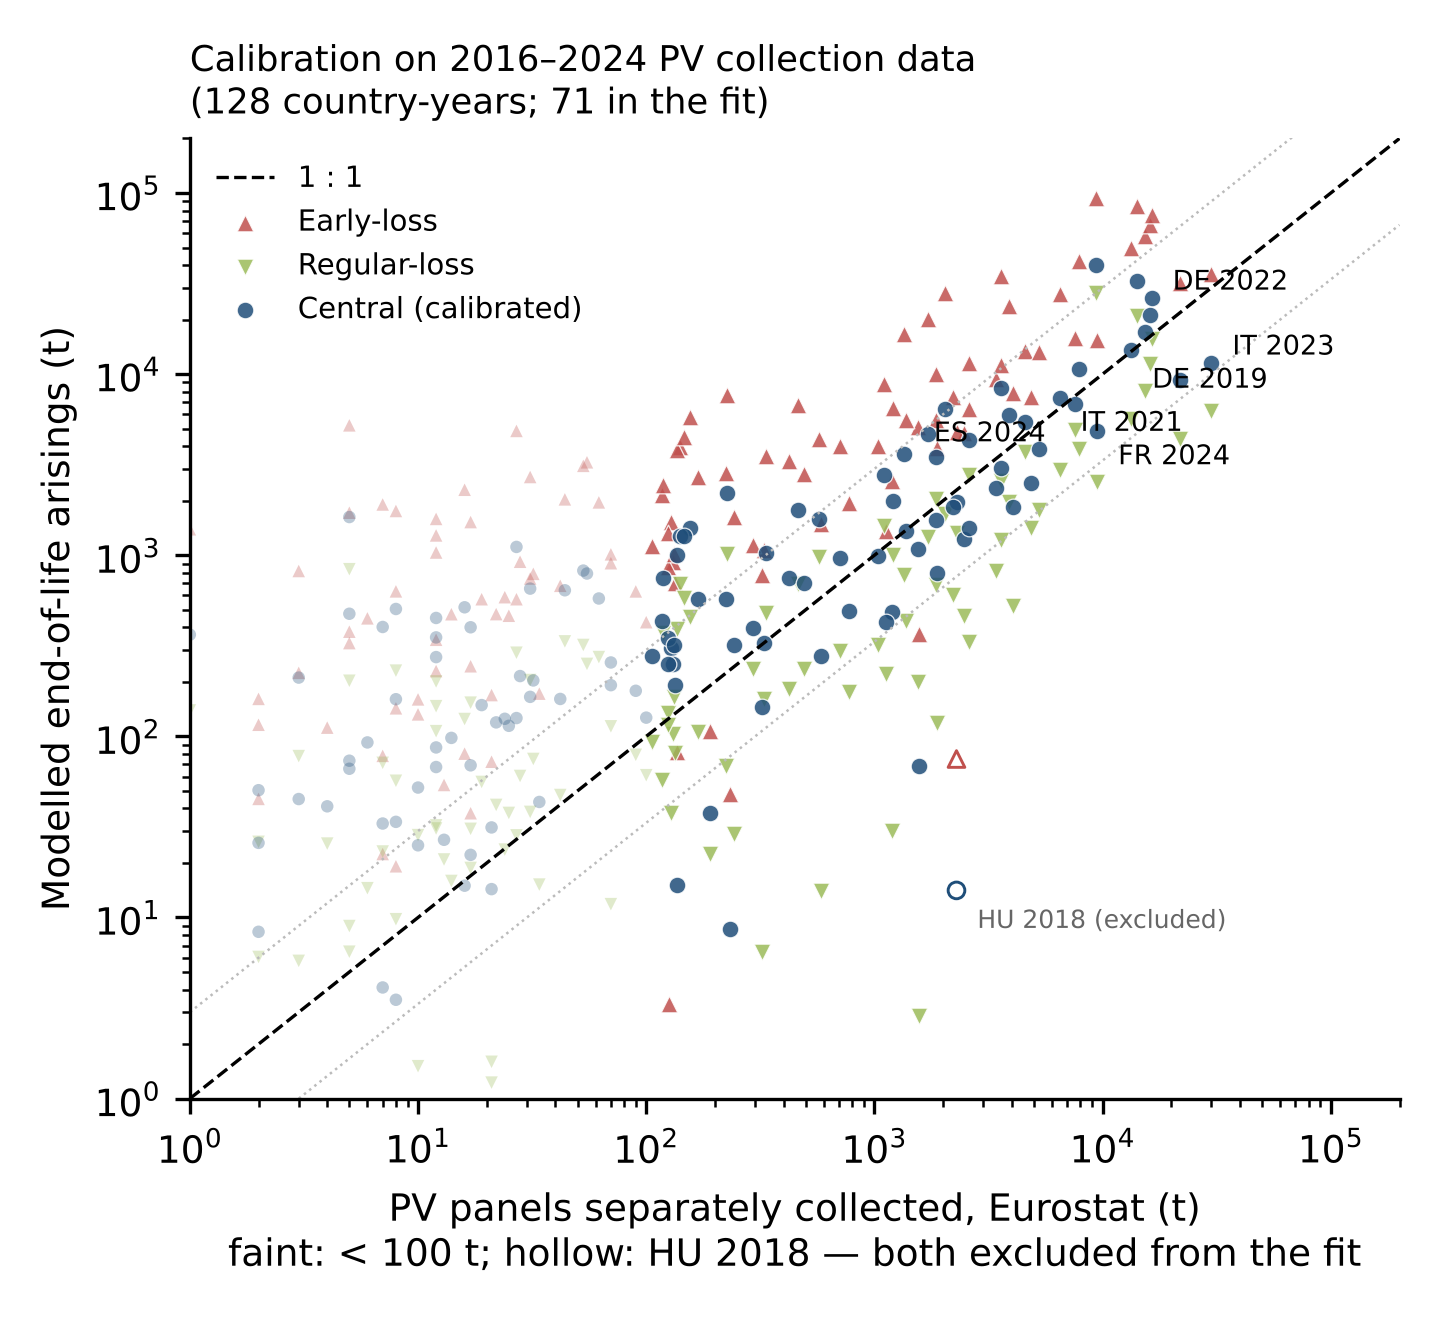
\includegraphics[width=0.9\columnwidth]{Figure_6.png}
\caption{Modelled end-of-life arisings versus PV panels separately collected (Eurostat, 2016--2024; 128 country-years with positive collection, of which 71 enter the fit) under the early-loss, regular-loss and calibrated central scenarios. Faint markers: below \SI{100}{t}; hollow markers: Hungary 2018, excluded. Dotted lines mark a factor of three.}\label{fig:valid}\end{figure}

\subsubsection{The EU-27 wave} Under the central scenario with continued deployment, cumulative arisings reach \SI{1.4}{Mt} by 2030, \SI{7.2}{Mt} by 2040 and \SI{20.9}{Mt} by 2050 (early-loss 3.2, 11.1 and 25.9; regular-loss 1.0, 6.4 and 19.8), of which \SI{15.4}{Mt} comes from the stock already installed in 2024 (Fig.~\ref{fig:euwave}). Annual arisings rise monotonically to about \SI{1.8}{Mt} per year in 2050; because deployment has kept growing, there is no EU-level peak before 2050 and the wave is better described as a rising tide whose onset differs across member states. The material streams cumulated to 2050 amount to roughly \SI{15.8}{Mt} of glass, \SI{2.1}{Mt} of polymers, \SI{1.7}{Mt} of aluminium, \SI{1.05}{Mt} of silicon, \SI{0.21}{Mt} of copper and about \SI{10}{kt} of silver.

\begin{figure*}[pos=t]\centering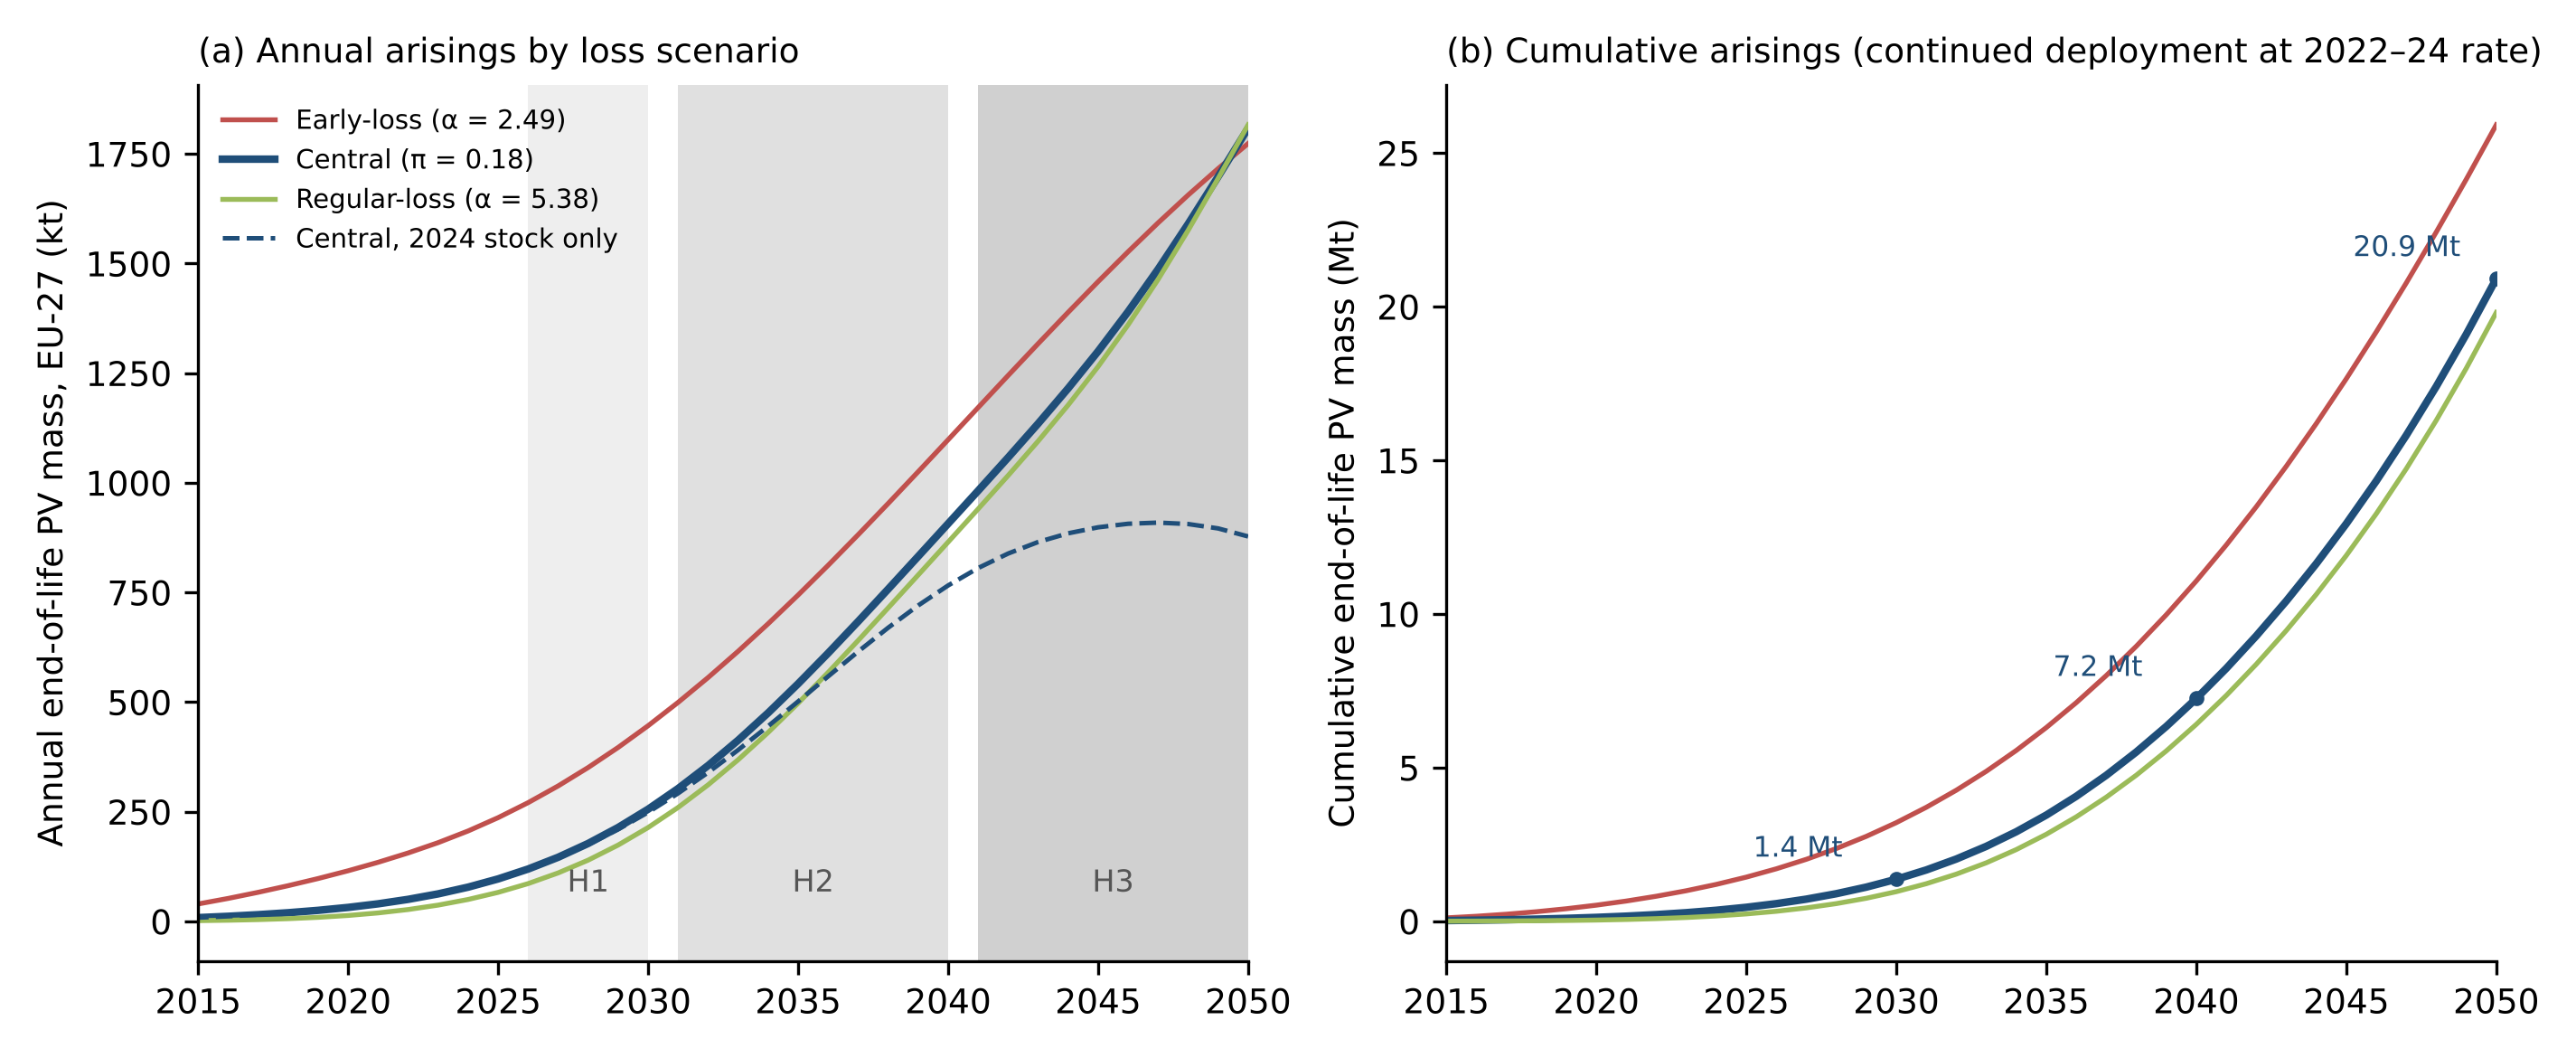
\includegraphics[width=\textwidth]{Figure_7.png}
\caption{EU-27 end-of-life PV mass: (a) annual arisings by loss scenario with the three strategy horizons shaded; (b) cumulative arisings under continued deployment at the 2022--2024 rate.}\label{fig:euwave}\end{figure*}

\subsubsection{Country waves} Table~\ref{tab:wave} and Fig.~\ref{fig:cwaves} give the national picture. Onset arrives in 2029 in Czechia, 2030 in Germany, Italy and Slovakia, 2031 in Belgium and Luxembourg, 2032 in France, Greece and Spain, and last, in 2038, in Ireland and Latvia; midpoints run from 2039 to 2046. Germany alone accounts for \SI{6.7}{Mt} by 2050 (p10--p90 \SIrange{5.5}{8.0}{Mt}), followed by Italy (2.8), Spain (2.3), France (1.7), the Netherlands (1.4) and Poland (1.3). Per capita by 2040, Germany (\SI{36}{kg}) is followed by Italy and Belgium (\SI{21}{kg}), Greece, the Netherlands and Luxembourg (17--\SI{18}{kg}), and Czechia, Spain, Austria and Bulgaria (13--\SI{14}{kg}); Romania, Ireland, Croatia and Finland are at or below \SI{2.5}{kg}.

\begin{figure}[pos=t]\centering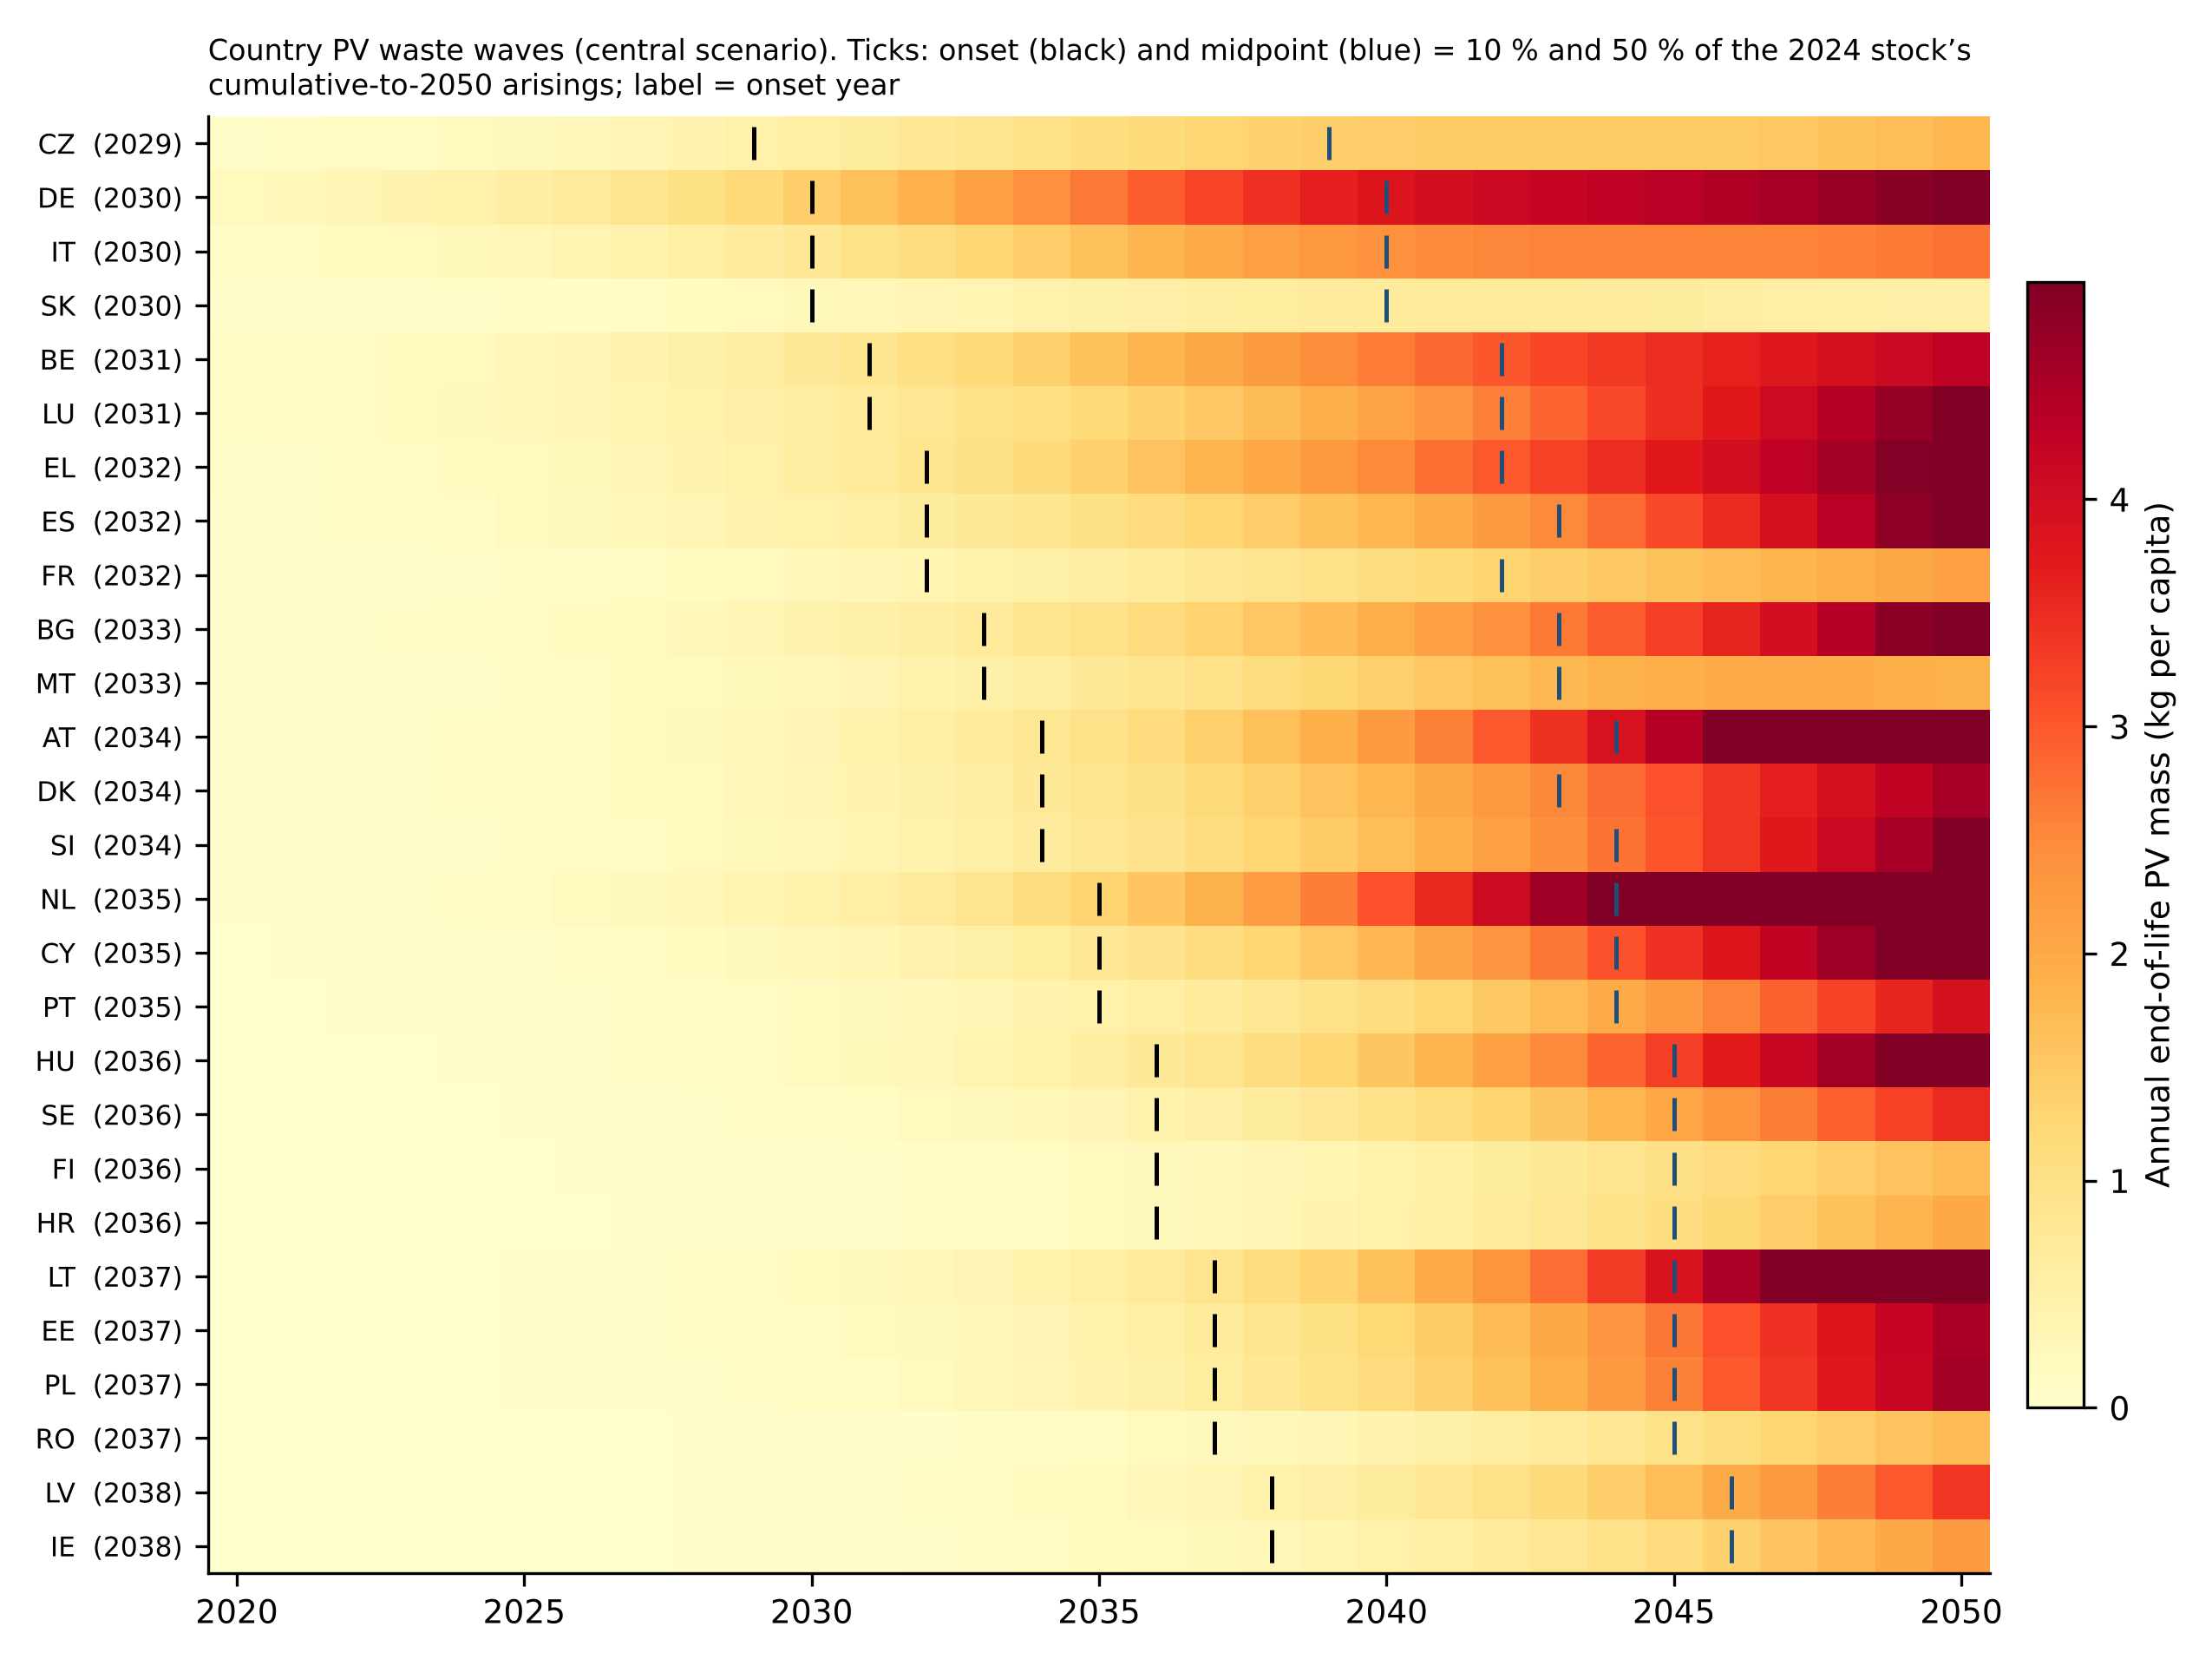
\includegraphics[width=\columnwidth]{Figure_8.png}
\caption{Annual end-of-life PV mass per capita by member state, ordered by onset year (central scenario). Black tick: onset, the year in which cumulative arisings from the stock installed by 2024 reach 10\,\% of that stock's cumulative-to-2050 arisings; blue tick: midpoint (50\,\%).}\label{fig:cwaves}\end{figure}

\begin{table*}[pos=t]\centering\scriptsize
\caption{Projected end-of-life photovoltaic module mass by member state (central scenario, continued deployment at the 2022--2024 rate): installed capacity 2024, mass of the 2024 stock, cumulative arisings by 2030/2040/2050 (kt) with Monte Carlo p10--p90 range for 2050 (EU-27 row: quantiles of the EU-total draws), cumulative mass per capita by 2040 (Eurostat population on 1 January 2024 as retrieved on 20 October 2026), and wave timing of the stock installed by 2024 (onset = year in which that stock's cumulative arisings reach 10\,\% of its cumulative-to-2050 arisings; midpoint = 50\,\%). MS: member state.}
\label{tab:wave}
\begin{adjustbox}{max width=\linewidth}\begin{tabular}{@{}lrrrrrrrcc@{}}\toprule
MS & GW$_{2024}$ & Stock (kt) & 2030 & 2040 & 2050 & p10--p90 & kg/cap$_{2040}$ & Onset & Mid \\ \midrule
DE & 91.2 & 7063 & 673 & 3000 & 6710 & 5547--7997 & 35.9 & 2030 & 2040 \\
IT & 35.4 & 2821 & 249 & 1252 & 2778 & 2324--3275 & 21.2 & 2030 & 2040 \\
ES & 35.8 & 2361 & 122 & 657 & 2333 & 1642--3263 & 13.5 & 2032 & 2043 \\
FR & 25.3 & 1788 & 88 & 546 & 1686 & 1285--2153 & 8.0 & 2032 & 2042 \\
NL & 24.8 & 1620 & 37 & 322 & 1409 & 996--1881 & 17.9 & 2035 & 2044 \\
PL & 21.7 & 1309 & 15 & 208 & 1254 & 804--1868 & 5.7 & 2037 & 2045 \\
BE & 9.6 & 710 & 44 & 248 & 669 & 530--825 & 21.0 & 2031 & 2042 \\
EL & 8.8 & 614 & 30 & 189 & 596 & 448--781 & 18.2 & 2032 & 2042 \\
AT & 8.9 & 563 & 15 & 122 & 563 & 379--817 & 13.4 & 2034 & 2044 \\
HU & 7.2 & 447 & 7 & 78 & 419 & 279--599 & 8.2 & 2036 & 2045 \\
PT & 5.6 & 351 & 9 & 74 & 353 & 234--519 & 6.6 & 2035 & 2044 \\
CZ & 4.0 & 317 & 34 & 153 & 321 & 267--390 & 14.0 & 2029 & 2039 \\
BG & 4.6 & 301 & 12 & 85 & 313 & 220--445 & 13.1 & 2033 & 2043 \\
SE & 4.8 & 297 & 5 & 52 & 289 & 188--425 & 4.9 & 2036 & 2045 \\
DK & 3.9 & 266 & 9 & 69 & 262 & 187--353 & 11.5 & 2034 & 2043 \\
RO & 4.3 & 253 & 3 & 39 & 243 & 154--367 & 2.0 & 2037 & 2045 \\
LT & 2.4 & 140 & 2 & 23 & 150 & 92--241 & 8.1 & 2037 & 2045 \\
SI & 1.4 & 92 & 3 & 23 & 93 & 64--132 & 10.6 & 2034 & 2044 \\
IE & 1.3 & 76 & 1 & 12 & 82 & 50--133 & 2.2 & 2038 & 2046 \\
FI & 1.2 & 77 & 1 & 14 & 75 & 49--110 & 2.5 & 2036 & 2045 \\
SK & 0.7 & 71 & 7 & 34 & 68 & 59--77 & 6.3 & 2030 & 2040 \\
HR & 0.9 & 54 & 1 & 10 & 56 & 36--89 & 2.5 & 2036 & 2045 \\
EE & 0.9 & 54 & 1 & 9 & 49 & 32--70 & 6.3 & 2037 & 2045 \\
CY & 0.8 & 48 & 1 & 10 & 46 & 31--64 & 10.4 & 2035 & 2044 \\
LV & 0.7 & 37 & 0 & 6 & 42 & 25--70 & 3.0 & 2038 & 2046 \\
LU & 0.5 & 38 & 2 & 11 & 36 & 27--47 & 17.0 & 2031 & 2042 \\
MT & 0.2 & 18 & 1 & 5 & 16 & 13--19 & 9.6 & 2033 & 2043 \\
\midrule EU-27 & 307 & 21785 & 1369 & 7249 & 20912 & 15969--26944 & & & \\
\bottomrule\end{tabular}\end{adjustbox}\end{table*}


\subsection{Coupling: readiness gap and archetypes}\label{sec:resGap}
Figure~\ref{fig:map} places each member state on the urgency--readiness plane and Table~\ref{tab:gap} ranks the readiness gap (see also Fig.~\ref{fig:gapmat}). Urgency and readiness are only weakly aligned: the earliest and heaviest waves fall on a mixture of leaders (Germany, Italy, Belgium) and converging states (Greece, Czechia, Bulgaria, Spain, Slovakia). Greece has the largest gap (0.68, p10--p90 0.58--0.85), followed by Bulgaria (0.49, 0.43--0.62) and Cyprus (0.42, 0.36--0.57). The marginal bands overlap: Greece's with Bulgaria's, and Bulgaria's and Cyprus's with each other and with those of several states ranked between fourth and fourteenth. The bands are, however, computed from draws in which the lifetime shape, scale and mass factor are common to all member states, so the question is how often the ranking changes across draws, not whether the bands overlap. Across the 600 joint draws Greece ranks first, Bulgaria second and Cyprus third in every draw (Table~\ref{tab:gap}, rank-range column). Fourth place is not separable: Germany (0.382, band 0.32--0.45) and Malta (0.380) take it in 44\,\% and 41\,\% of draws, and Germany's rank ranges from fourth to eighth. Germany's case is nevertheless distinctive: the highest urgency in the Union, $\mathrm{urg}=0.98$, is only partly offset by leader-level readiness of 0.61. Malta, Portugal, Czechia, Spain, Slovakia and Denmark complete the top ten. The Netherlands, Belgium, Luxembourg, France, Estonia and Austria have the smallest gaps. The three archetypes are: L, the eight consolidated leaders (onset 2030--2037, \SI{13.9}{Mt} by 2050, mean readiness 0.72, mean gap 0.18); EW, ten converging states with onset at or before 2035 (Greece, Bulgaria, Cyprus, Malta, Portugal, Spain, Czechia, Slovakia, Denmark, Slovenia; \SI{4.4}{Mt}; readiness 0.30; gap 0.40); and LW, nine converging states with onset 2036--2038 (Hungary, Romania, Lithuania, Finland, Croatia, Sweden, Poland, Ireland, Latvia; \SI{2.6}{Mt}; readiness 0.33; gap 0.25).

\begin{figure}[pos=t]\centering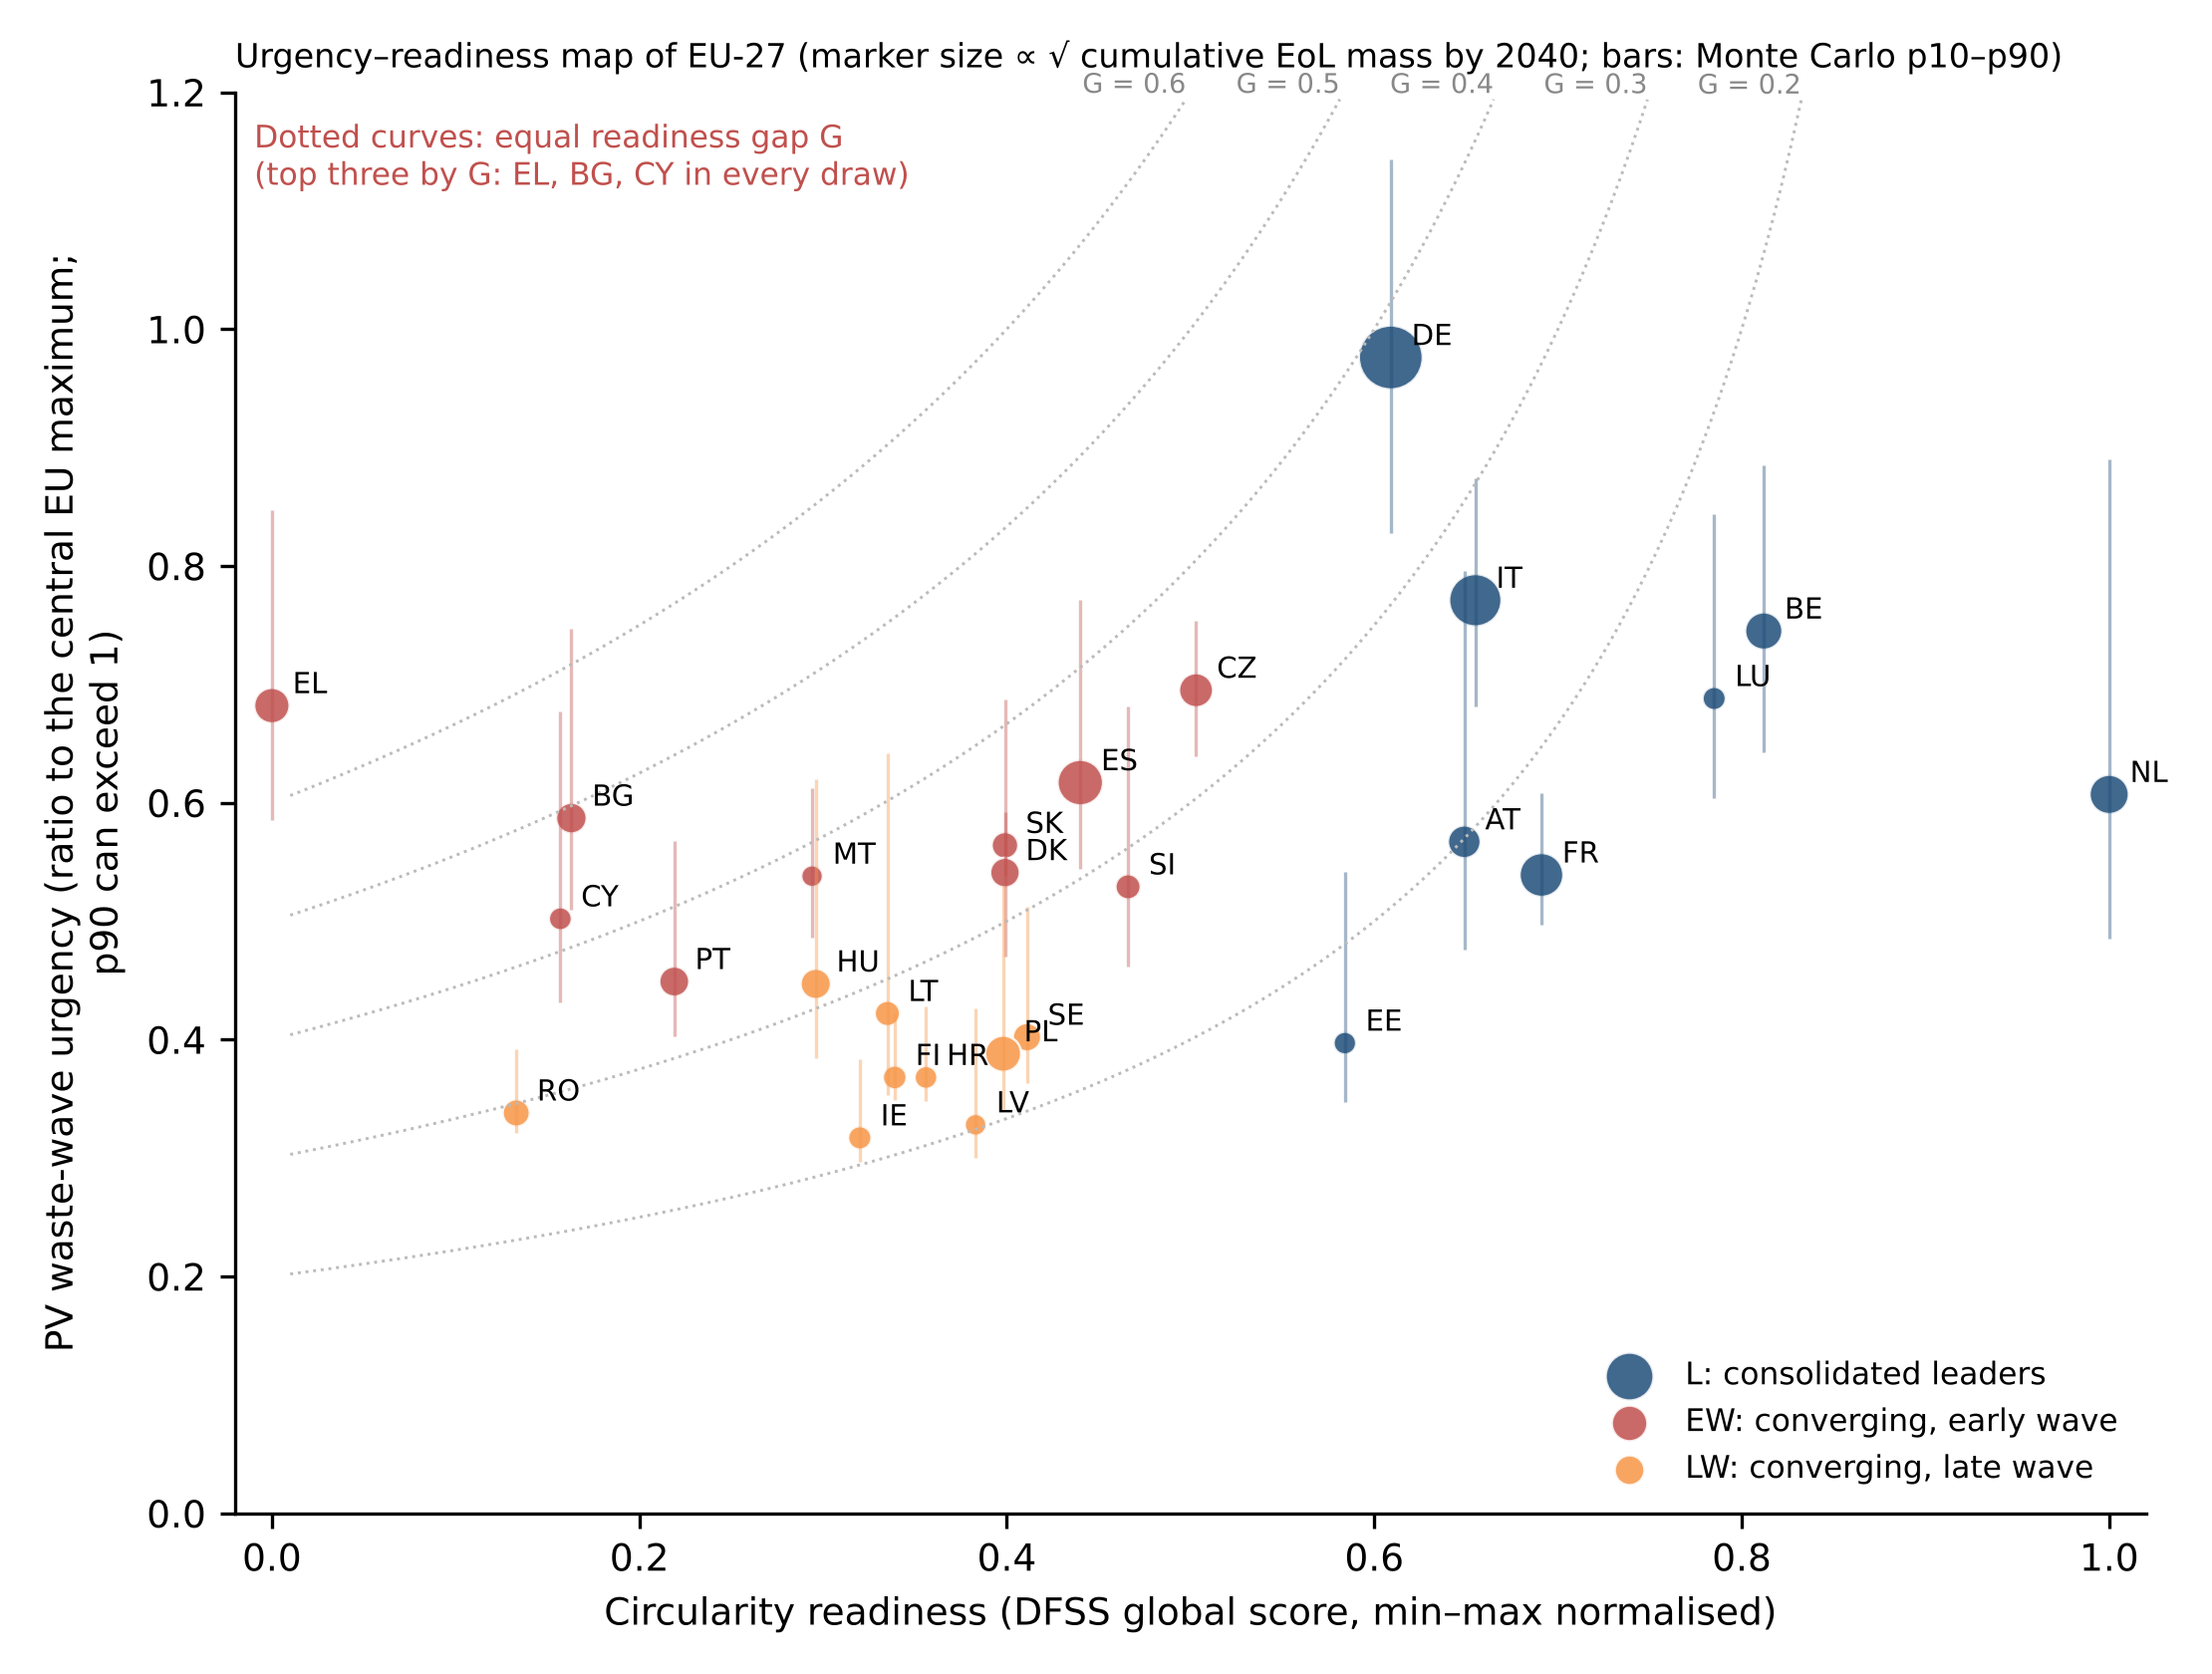
\includegraphics[width=\columnwidth]{Figure_9.png}
\caption{Urgency--readiness map of EU-27. Marker size is proportional to the square root of cumulative arisings by 2040; bars give the Monte Carlo p10--p90 range of urgency, which is normalised to the central EU maximum and can therefore exceed one; dotted curves are lines of equal readiness gap $G$.}\label{fig:map}\end{figure}

\begin{table*}[pos=t]\centering\footnotesize
\caption{Readiness gap $G(u)=\mathrm{urg}(u)\,[1-\mathrm{rdy}(u)]$ of EU-27 member states, with urgency (cumulative arisings per capita by 2040 and onset earliness, ratio-normalised), readiness (DFSS global score, min--max normalised), Monte Carlo p10--p90 band of the gap, the range of ranks attained across the 600 joint draws (parameters are common to all member states within a draw, so bands can overlap while ranks are stable), and archetype (L consolidated leaders; EW converging, early wave; LW converging, late wave). MS: member state.}
\label{tab:gap}
\begin{adjustbox}{max width=\linewidth}\begin{tabular}{@{}rlcccccc@{}}\toprule
Rank & MS & Urgency & Readiness & Gap & p10--p90 & Rank range & Archetype \\ \midrule
1 & EL & 0.68 & 0.00 & 0.682 & 0.58--0.85 & 1--1 & EW \\
2 & BG & 0.59 & 0.16 & 0.492 & 0.43--0.62 & 2--2 & EW \\
3 & CY & 0.50 & 0.16 & 0.424 & 0.36--0.57 & 3--3 & EW \\
4 & DE & 0.98 & 0.61 & 0.382 & 0.32--0.45 & 4--8 & L \\
5 & MT & 0.54 & 0.29 & 0.380 & 0.34--0.43 & 4--10 & EW \\
6 & PT & 0.45 & 0.22 & 0.350 & 0.32--0.44 & 4--9 & EW \\
7 & CZ & 0.69 & 0.50 & 0.346 & 0.32--0.38 & 6--12 & EW \\
8 & ES & 0.62 & 0.44 & 0.345 & 0.30--0.43 & 6--9 & EW \\
9 & SK & 0.56 & 0.40 & 0.339 & 0.32--0.36 & 5--15 & EW \\
10 & DK & 0.54 & 0.40 & 0.325 & 0.28--0.41 & 9--11 & EW \\
11 & HU & 0.45 & 0.30 & 0.315 & 0.27--0.44 & 4--12 & LW \\
12 & RO & 0.34 & 0.13 & 0.293 & 0.28--0.34 & 10--15 & LW \\
13 & SI & 0.53 & 0.47 & 0.282 & 0.25--0.36 & 11--14 & EW \\
14 & LT & 0.42 & 0.34 & 0.281 & 0.23--0.43 & 4--15 & LW \\
15 & IT & 0.77 & 0.66 & 0.266 & 0.23--0.30 & 12--19 & L \\
16 & FI & 0.37 & 0.34 & 0.243 & 0.23--0.28 & 14--19 & LW \\
17 & SE & 0.40 & 0.41 & 0.237 & 0.21--0.30 & 16--18 & LW \\
18 & HR & 0.37 & 0.36 & 0.237 & 0.22--0.28 & 16--20 & LW \\
19 & PL & 0.39 & 0.40 & 0.234 & 0.20--0.32 & 13--19 & LW \\
20 & IE & 0.32 & 0.32 & 0.215 & 0.20--0.26 & 20--22 & LW \\
21 & LV & 0.33 & 0.38 & 0.202 & 0.18--0.26 & 21--22 & LW \\
22 & AT & 0.57 & 0.65 & 0.199 & 0.17--0.28 & 17--22 & L \\
23 & FR & 0.54 & 0.69 & 0.167 & 0.15--0.19 & 23--25 & L \\
24 & EE & 0.40 & 0.58 & 0.165 & 0.14--0.23 & 23--24 & L \\
25 & LU & 0.69 & 0.79 & 0.148 & 0.13--0.18 & 24--25 & L \\
26 & BE & 0.74 & 0.81 & 0.140 & 0.12--0.17 & 26--26 & L \\
27 & NL & 0.61 & 1.00 & 0.000 & 0.00--0.00 & 27--27 & L \\
\bottomrule\end{tabular}\end{adjustbox}\end{table*}


\begin{figure*}[pos=t]\centering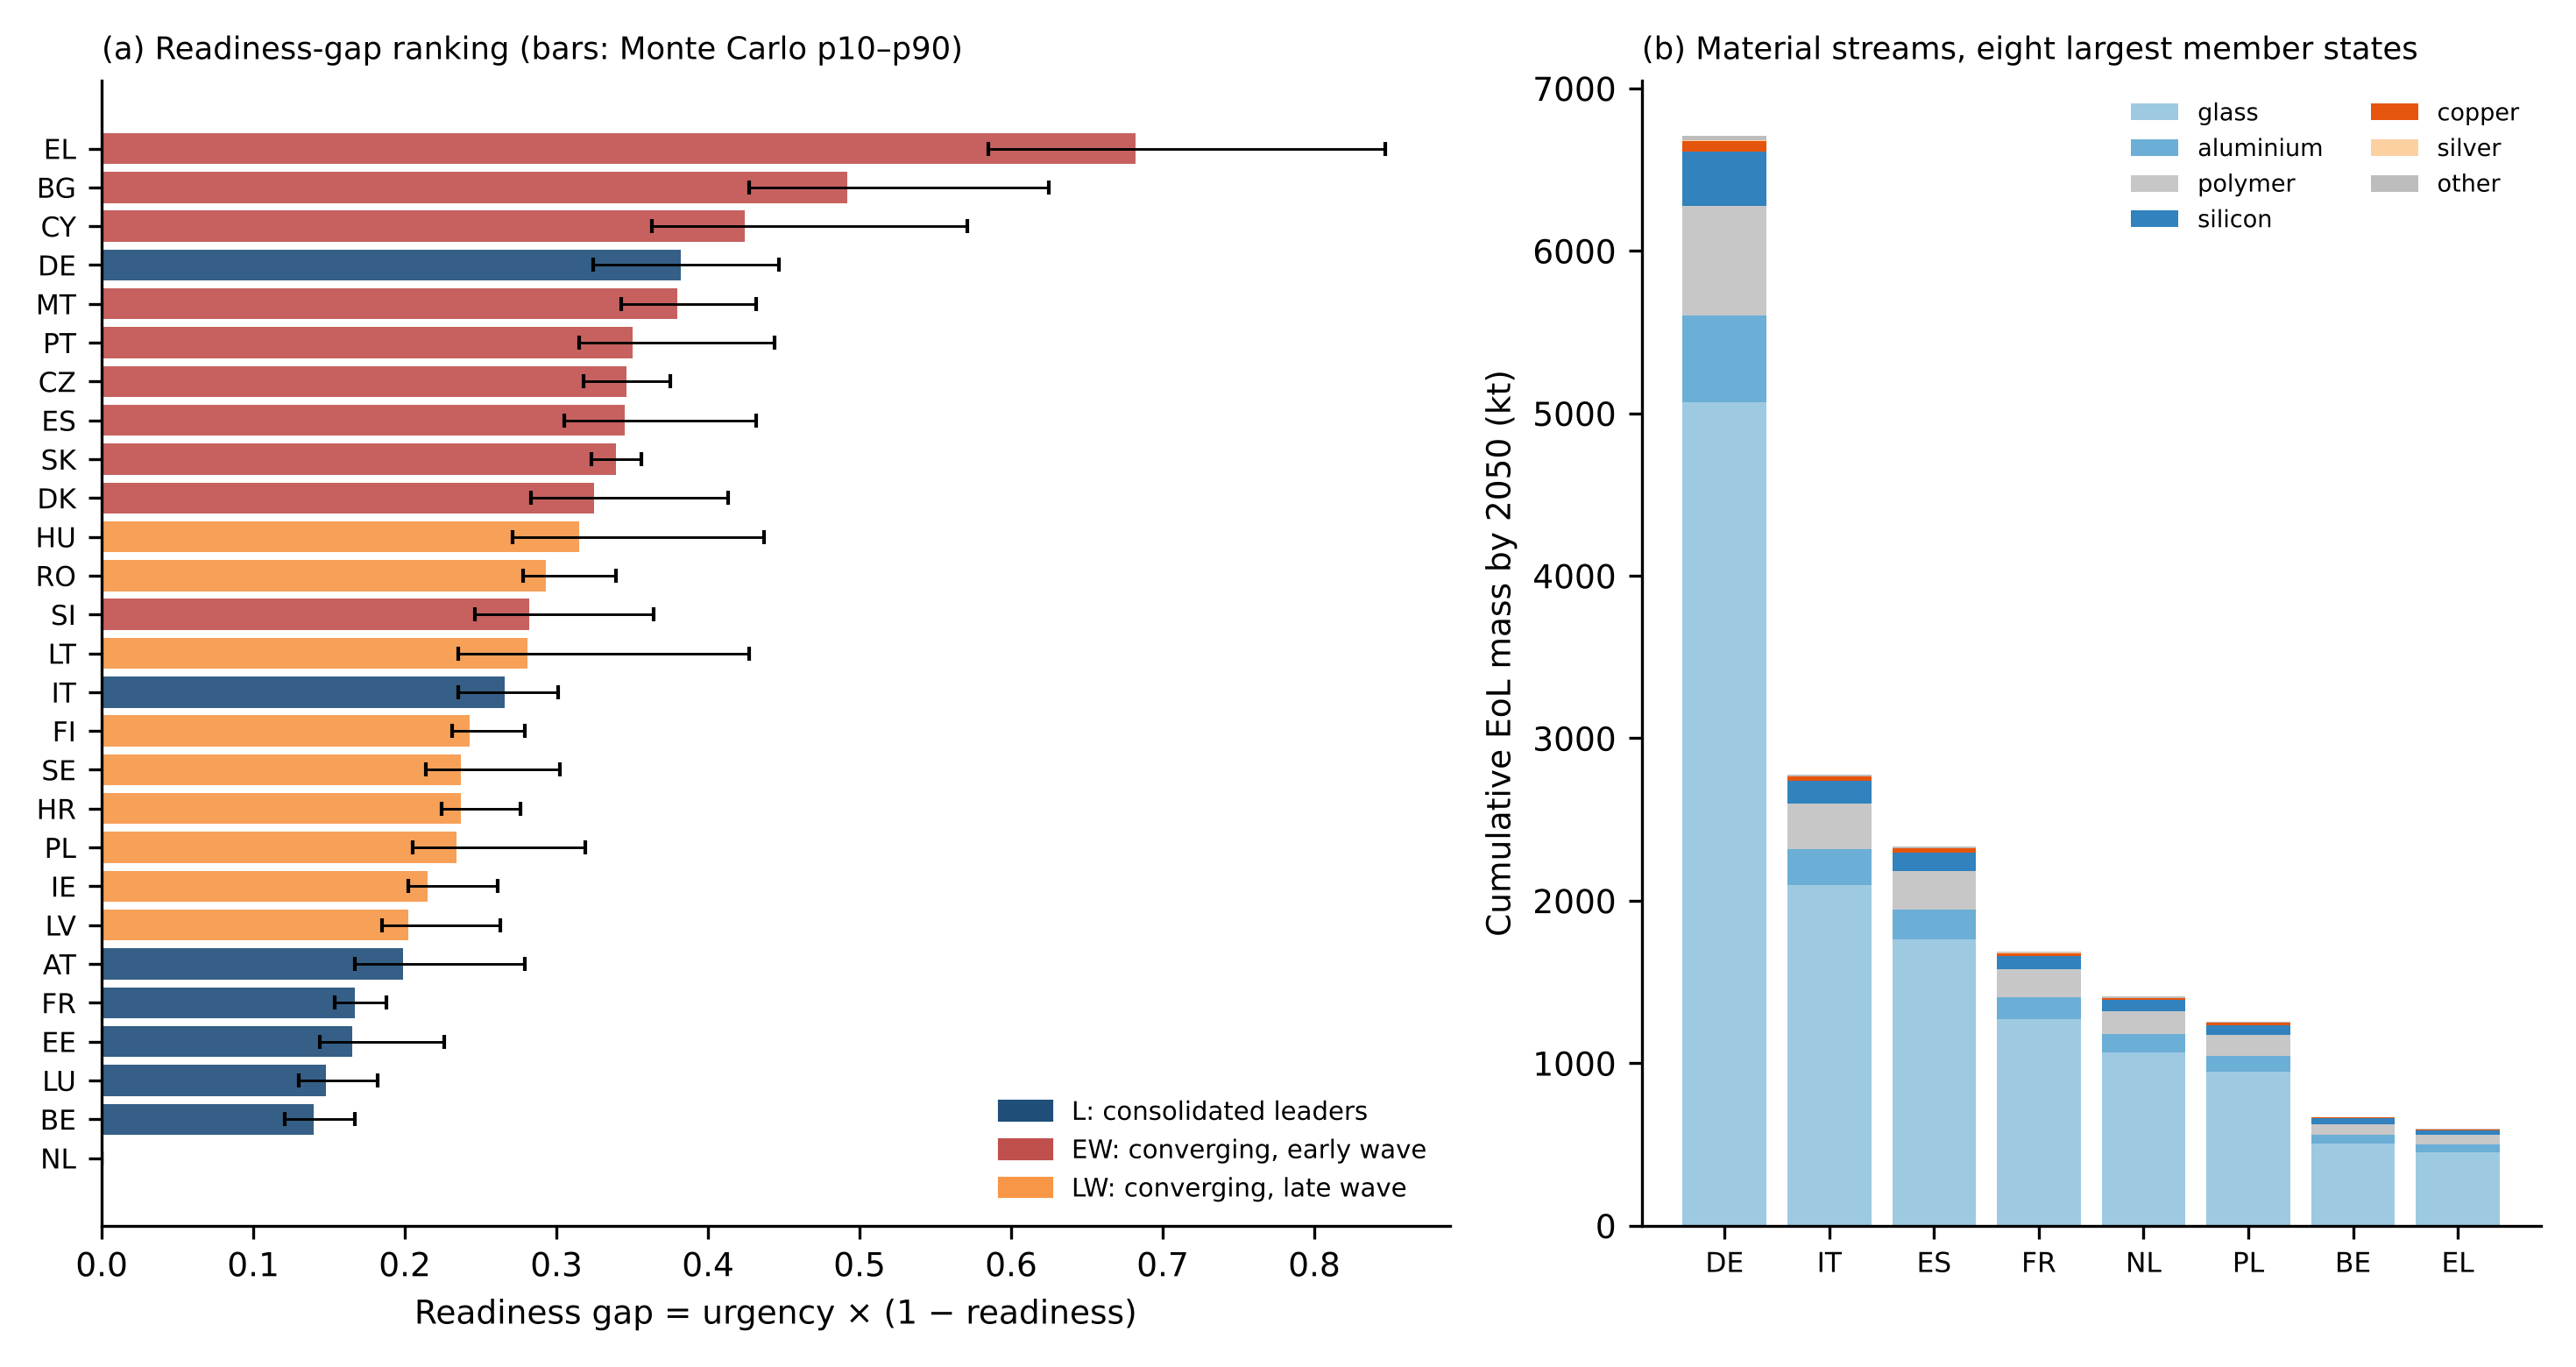
\includegraphics[width=\textwidth]{Figure_10.png}
\caption{(a) Readiness-gap ranking with Monte Carlo bands, coloured by archetype; (b) material streams cumulated to 2050 for the eight largest member states.}\label{fig:gapmat}\end{figure*}

\subsection{Layer C: strategy activation by archetype and horizon}\label{sec:resC}
Table~\ref{tab:cost} translates the Layer~B arisings into an indicative net treatment bill per archetype and horizon under the bulk-recycling, high-value-recycling and disposal pathways, using the Layer~C cost ranges. For the EU as a whole the 2026--2030 bill is small under any pathway (EUR 0.1--0.4 billion, graded mean), because arisings are only \SI{0.9}{Mt}; it becomes material in 2031--2040 (EUR 1.0--1.3 billion) and large in 2041--2050, where bulk recycling of \SI{13.7}{Mt} costs about EUR 2.1 billion and disposal, with rising gate fees, about EUR 4.2 billion, while high-value recycling spans a wide fuzzy support (EUR $-5.5$ to $+8.2$ billion) whose sign depends on whether silicon and silver revenues materialise at scale \citep{markert2020,dadamo2017,deng2019}. The bill is concentrated in the leaders (two-thirds of arisings) but the early-wave group faces EUR 0.3--1.0 billion in 2041--2050 from a base of the weakest readiness.

Table~\ref{tab:proxies} reports the institutional capacities that enter this layer. The leaders exceed both converging groups on every criterion ($\kappa$ 0.55--0.72 against 0.41--0.54 for the early-wave group and 0.50--0.56 for the late-wave group), and the early-wave group is weakest on all four, with the largest shortfalls in enforcement and social acceptance; this is the Layer~A readiness result seen from an independent dataset of WEEE and governance statistics. Table~\ref{tab:activation} and Fig.~\ref{fig:timeline} give the DFSS local ranks per horizon and the global Phase-3 rank for each archetype; Supplementary Fig.~S2 shows the supports of the fuzzy local scores. Three patterns hold across archetypes (Table~\ref{tab:synthesis}). Repair and refurbishment for domestic reuse ($a_1$) ranks first in 2026--2030 and 2031--2040 everywhere, sustained by negative or near-zero net cost, the highest avoided emissions and employment, and moderate institutional requirements; it falls to second (leaders) or third (converging) in 2041--2050 as the vintages reaching end of life become too old to justify re-certification and acceptance becomes decisive. High-value recycling ($a_5$) ranks first in 2041--2050 in every archetype and already second everywhere in 2031--2040, driven by the activation of the critical-raw-material criterion, falling net cost as silicon and silver recovery is credited, and a diminishing dependence on first-mover actors; cascaded second use ($a_2$) is second or third throughout. Landfill and incineration ($a_7$) is last throughout; its fuzzy support is separated from every other alternative in the leader archetype, where strong regulation, enforcement and participation work against it, whereas in the converging archetypes it overlaps the lower tails of export, take-back and bulk recycling (Supplementary Fig.~S2). Export for second life ($a_3$) ranks third (leaders) or fourth (converging) in 2026--2030, when its low cost and minimal actor requirement weigh most; it slips to fifth in 2031--2040 for the leaders and the early-wave group but stays fourth for the late-wave group, and to fifth or sixth in 2041--2050 as the enforcement and critical-raw-material criteria bind, for a global rank of fourth (late wave) or fifth. It is therefore a mid-table option throughout rather than a pathway that is competitive only in the current decade; its relative position is strongest now and in the late-wave states, and it never approaches the top two. Formalised take-back ($a_6$) ranks fourth to sixth: as an enabling pathway it scores low on the treatment-side criteria, which is a limitation of evaluating it alongside treatment pathways, but its rank rises or holds in every archetype as the horizon advances (fifth, fourth, fourth for the leaders; sixth, fourth, fourth for the early wave; sixth, fifth, fourth for the late wave). The top and bottom of the ordering are robust: across weight schemes and thirty runs of independent $\pm20\,\%$ perturbation of all criterion values, the top-ranked alternative is reproduced in 97\,\% of archetype-horizon cells, and fuzzy TOPSIS agrees with the DFSS ordering at $\tau_b=0.96$. The middle of the ordering is not: Kendall $\tau_b$ with the primary specification averages 0.77 (minimum 0.68) under perturbation, because the local scores of $a_2$, $a_3$, $a_4$ and $a_6$ lie within 0.05 of one another in several cells (Supplementary Fig.~S2). Equal and institution-heavy weightings agree with the primary ordering at $\tau_b=0.94$ and $0.91$. Because $|A_t|$ varies only between eight and nine in this layer, the pooled aggregation coincides with the DFSS global ranking; the cardinality bias documented in Layer~A does not recur here.

\begin{figure*}[pos=t]\centering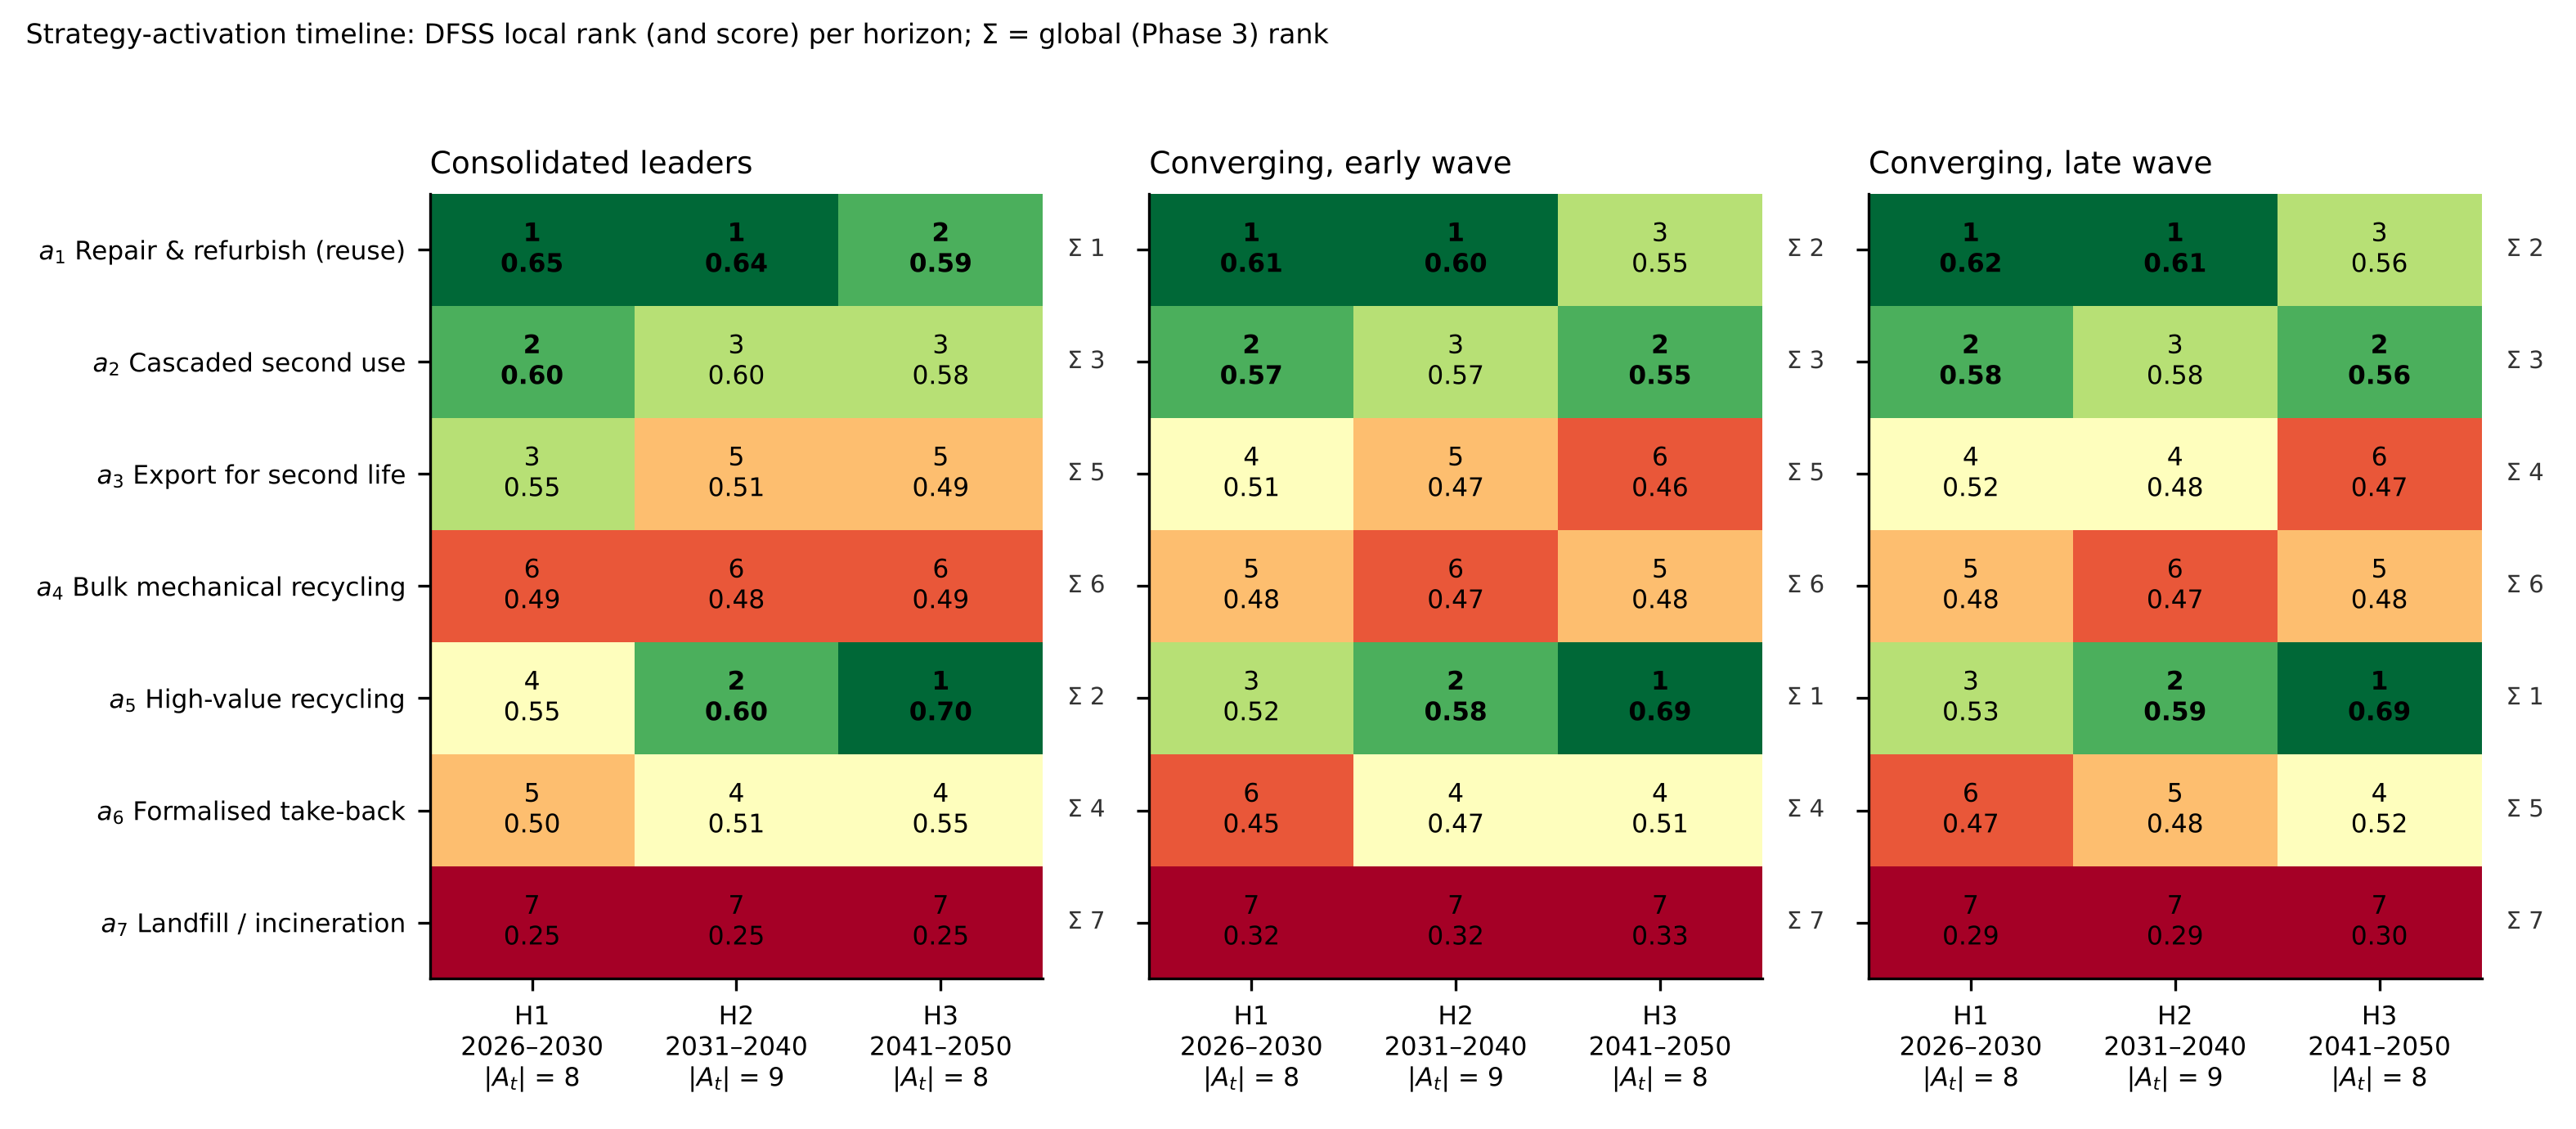
\includegraphics[width=\textwidth]{Figure_11.png}
\caption{Strategy-activation timeline: DFSS local rank and graded-mean score per horizon and archetype; $\Sigma$ gives the global Phase-3 rank.}\label{fig:timeline}\end{figure*}


\begin{table*}[pos=t]\centering\footnotesize
\caption{Indicative net treatment bill (EUR billion) by archetype and horizon under three pathways: central-scenario arisings (kt) times the literature-derived net cost per tonne (graded mean, with [lower; upper] bounds of the triangular fuzzy number; negative values are net revenue), with the archetype cost factor used in the decision matrix (0.90, 1.00, 1.15) applied to positive net costs and its reciprocal to net revenues; the EU-27 row is unscaled. Bulk = mechanical recycling ($a_4$); HV = high-value recycling ($a_5$); Landfill = disposal ($a_7$) with rising gate fees. Net costs exclude collection logistics, which \citet{markert2020} find to dominate private end-of-life cost.}
\label{tab:cost}
\begin{adjustbox}{max width=\linewidth}\begin{tabular}{@{}llrlll@{}}\toprule
Archetype & Horizon & kt & Bulk & HV & Landfill \\ \midrule
Leaders ($\times$0.90) & H1 2026--2030 & 731 & 0.14 [0.03; 0.26] & 0.27 [-0.16; 0.72] & 0.09 [0.03; 0.16] \\
 & H2 2031--2040 & 4,401 & 0.70 [0.12; 1.39] & 0.81 [-1.47; 3.17] & 0.83 [0.40; 1.39] \\
 & H3 2041--2050 & 8,392 & 1.18 [0.15; 2.42] & 0.64 [-3.73; 4.53] & 2.33 [1.13; 3.78] \\
\addlinespace
Converging, early ($\times$1.00) & H1 2026--2030 & 154 & 0.03 [0.01; 0.06] & 0.06 [-0.03; 0.17] & 0.02 [0.01; 0.04] \\
 & H2 2031--2040 & 1,071 & 0.19 [0.03; 0.37] & 0.23 [-0.32; 0.86] & 0.22 [0.11; 0.37] \\
 & H3 2041--2050 & 3,102 & 0.49 [0.06; 0.99] & 0.31 [-1.24; 1.86] & 0.96 [0.47; 1.55] \\
\addlinespace
Converging, late ($\times$1.15) & H1 2026--2030 & 28 & 0.01 [0.00; 0.01] & 0.01 [-0.00; 0.04] & 0.00 [0.00; 0.01] \\
 & H2 2031--2040 & 408 & 0.08 [0.01; 0.16] & 0.11 [-0.11; 0.38] & 0.10 [0.05; 0.16] \\
 & H3 2041--2050 & 2,169 & 0.39 [0.05; 0.80] & 0.29 [-0.75; 1.50] & 0.77 [0.37; 1.25] \\
\addlinespace
EU-27 (unscaled) & H1 2026--2030 & 913 & 0.19 [0.05; 0.37] & 0.38 [-0.18; 1.00] & 0.12 [0.05; 0.23] \\
 & H2 2031--2040 & 5,880 & 1.04 [0.18; 2.06] & 1.27 [-1.76; 4.70] & 1.23 [0.59; 2.06] \\
 & H3 2041--2050 & 13,663 & 2.14 [0.27; 4.37] & 1.37 [-5.47; 8.20] & 4.21 [2.05; 6.83] \\
\addlinespace
\bottomrule\end{tabular}\end{adjustbox}\end{table*}

\begin{table*}[pos=t]\centering\scriptsize
\caption{Strategy-activation results per archetype: DFSS local rank (graded-mean score in parentheses) for horizons H1 2026--2030, H2 2031--2040, H3 2041--2050, and global Phase-3 rank $\Sigma$ (ranks are computed on unrounded scores). Institutional criteria C1--C4 are derived from public-data proxies (Table~\ref{tab:proxies}).}
\label{tab:activation}
\begin{adjustbox}{max width=\linewidth}\begin{tabular}{@{}lcccc@{\hspace{18pt}}cccc@{\hspace{18pt}}cccc@{}}\toprule
 & \multicolumn{4}{c}{L: consolidated leaders} & \multicolumn{4}{c}{EW: converging, early wave} & \multicolumn{4}{c}{LW: converging, late wave} \\ \cmidrule(lr){2-5}\cmidrule(lr){6-9}\cmidrule(lr){10-13}
Alternative & H1 & H2 & H3 & $\Sigma$ & H1 & H2 & H3 & $\Sigma$ & H1 & H2 & H3 & $\Sigma$ \\ \midrule
$a_1$ Repair \& refurbish (reuse) & 1 (0.65) & 1 (0.64) & 2 (0.59) & 1 & 1 (0.61) & 1 (0.60) & 3 (0.55) & 2 & 1 (0.62) & 1 (0.61) & 3 (0.56) & 2 \\
$a_2$ Cascaded second use & 2 (0.60) & 3 (0.60) & 3 (0.58) & 3 & 2 (0.57) & 3 (0.57) & 2 (0.55) & 3 & 2 (0.58) & 3 (0.58) & 2 (0.56) & 3 \\
$a_3$ Export for second life & 3 (0.55) & 5 (0.51) & 5 (0.49) & 5 & 4 (0.51) & 5 (0.47) & 6 (0.46) & 5 & 4 (0.52) & 4 (0.48) & 6 (0.47) & 4 \\
$a_4$ Bulk mechanical recycling & 6 (0.49) & 6 (0.48) & 6 (0.49) & 6 & 5 (0.48) & 6 (0.47) & 5 (0.48) & 6 & 5 (0.48) & 6 (0.47) & 5 (0.48) & 6 \\
$a_5$ High-value recycling & 4 (0.55) & 2 (0.60) & 1 (0.70) & 2 & 3 (0.52) & 2 (0.58) & 1 (0.69) & 1 & 3 (0.53) & 2 (0.59) & 1 (0.69) & 1 \\
$a_6$ Formalised take-back & 5 (0.50) & 4 (0.51) & 4 (0.55) & 4 & 6 (0.45) & 4 (0.47) & 4 (0.51) & 4 & 6 (0.47) & 5 (0.48) & 4 (0.52) & 5 \\
$a_7$ Landfill / incineration & 7 (0.25) & 7 (0.25) & 7 (0.25) & 7 & 7 (0.32) & 7 (0.32) & 7 (0.33) & 7 & 7 (0.29) & 7 (0.29) & 7 (0.30) & 7 \\
\bottomrule\end{tabular}\end{adjustbox}\end{table*}

\begin{table*}[pos=t]\centering\scriptsize
\caption{Synthesis across layers: archetype membership (ordered by readiness gap), onset range, cumulative arisings by 2050, mean readiness and gap, and the two highest-ranked strategies per horizon.}
\label{tab:synthesis}
\begin{adjustbox}{max width=\linewidth}\begin{tabular}{@{}lcp{4.2cm}ccccccc@{}}\toprule
Archetype & $n$ & Member states & Onset & Mt$_{2050}$ & Rdy & Gap & H1 & H2 & H3 \\ \midrule
L: consolidated leaders & 8 & DE, IT, AT, FR, EE, LU, BE, NL & 2030–2037 & 13.9 & 0.72 & 0.18 & $a_1$, $a_2$ & $a_1$, $a_5$ & $a_5$, $a_1$ \\
EW: converging, early wave & 10 & EL, BG, CY, MT, PT, CZ, ES, SK, DK, SI & 2029–2035 & 4.4 & 0.30 & 0.40 & $a_1$, $a_2$ & $a_1$, $a_5$ & $a_5$, $a_2$ \\
LW: converging, late wave & 9 & HU, RO, LT, FI, SE, HR, PL, IE, LV & 2036–2038 & 2.6 & 0.33 & 0.25 & $a_1$, $a_2$ & $a_1$, $a_5$ & $a_5$, $a_2$ \\
\bottomrule\end{tabular}\end{adjustbox}\end{table*}


\section{Discussion}\label{sec:discussion}

\subsection{What the framework revision did to the meaning of circularity}
The first finding is methodological but its content is political. About two-thirds of the movement in national circularity scores between 2020 and 2023 reflects the European Commission's decision to add footprint and resilience indicators to the monitoring framework, not changes in what member states did. The revision was well founded---circularity that ignores consumption footprints and import dependency is incomplete \citep{moraga2019,mayer2019}---but its effect on the ranking is large and systematic: consumption-intensive, high-income economies that had led on recycling rates and circular-sector investment move down, and lower-consumption economies move up, regardless of their waste-management performance. Table~\ref{tab:decomp} makes the consequence concrete: Croatia rises from seventeenth to thirteenth in the 2023 period ranking with a value effect of $-0.000$, Latvia from twentieth to eleventh with a structural effect twice its value effect, and Luxembourg falls from third to tenth with a value effect of $-0.003$. A member state reading its own progress off the Eurostat scoreboard across the revision would misattribute the change; a policy evaluation that back-imputed the new indicators would rewrite the past. The DFSS does neither. It keeps each window's judgement inside its own criteria set and makes the structural component of change explicit, which is what a monitoring framework that is expected to evolve requires.

The same logic applies to any renewable-energy circularity benchmark whose criteria will change---as they will, for instance, when PV Ecodesign requirements, the revised WEEE Directive and the Critical Raw Materials Act introduce new reportable quantities. The decomposition of Eq.~\eqref{eq:decomp} is a general tool for auditing such changes.

\subsection{Cost, environmental impact and resilience}
The three themes of this special issue map directly onto the layers. On \emph{cost}, the calibration in Section~\ref{sec:resB} matters more than the projection itself: at $\pi=0.18$ the EU is on a trajectory much closer to IRENA's regular-loss than early-loss curve for the coming decade, which implies that the 2026--2030 arisings on which collection and treatment capacity must be sized are roughly \SI{0.9}{Mt} rather than the \SI{1.8}{Mt} of the early-loss envelope (cumulative to 2030: 1.4 against \SI{3.2}{Mt}). Sizing to the early-loss envelope would over-invest in the near term by a factor of two; sizing to regular loss alone (\SI{0.7}{Mt}) would under-collect relative to what was observed in Germany, France and the Netherlands in 2019--2021. Italy's 2022--2023 collection shows the exception: where repowering incentives replace functioning modules, arisings run at the early-loss envelope and capacity must be sized accordingly, and the modules so replaced are the natural feedstock of the cascaded-second-use pathway. The activation results add the timing of cost exposure: reuse pathways are net-cost-negative or neutral through 2040 and dominate for that reason, while high-value recycling becomes economically defensible only as process cost falls and critical-raw-material recovery is credited.

On \emph{environmental impact}, the material streams give the stakes: some \SI{16}{Mt} of glass and \SI{1.7}{Mt} of aluminium are recoverable at bulk quality with existing processes, but the \SI{1.0}{Mt} of silicon and roughly \SI{10}{kt} of silver---the fractions whose recovery differentiates high-value from bulk recycling \citep{latunussa2016,deng2019,heath2020}---will be lost unless high-value capacity exists by around 2040, when the midpoints of the German, Czech, Italian and Slovak waves arrive. The activation timeline ranks high-value recycling second in 2031--2040 and first in 2041--2050 in every archetype; the environmental case is for bringing the transition forward in the EW archetype, whose wave arrives on the leaders' schedule but whose readiness does not.

On \emph{resilience}, the readiness gap is the operative measure. Greece, Bulgaria and Cyprus combine early or heavy waves with some of the weakest circular systems, and hold the first three places in every Monte Carlo draw. Germany, which shares fourth place with Malta, is a different kind of resilience problem: its readiness is high but the absolute volume, \SI{6.7}{Mt} by 2050 with onset in 2030, is without precedent, and the 2019--2022 collection data show that Germany's take-back collected about what the central scenario predicts in 2019--2020 and less thereafter. Silver and silicon recovery from that stream is, in tonnage, the largest single opportunity to reduce EU import dependency for PV-relevant materials.

\subsection{The instruments in play}
The recommendations that follow attach to a specific and currently moving regulatory context. Producer responsibility for PV modules rests on the WEEE Directive \citep{weee2012}, which brought PV panels into scope in 2012. In 2022 the Court of Justice declared its financing provision partially invalid for retroactivity in a preliminary ruling (Case C-181/20), and the 2024 amending directive confirmed that producers finance the management of panels placed on the market after 13 August 2012 while requiring the Commission to assess the need for a full revision by 31 December 2026 \citep{weee2024}; the Commission's evaluation of the Directive was published in July 2025 \citep{ec2025weee}. In the negotiation of the amendment the European Parliament called for a separate photovoltaic-panels category and for collection targets calculated on the basis of waste PV panels \emph{available for collection given their projected lifetime}, rather than on the quantity placed on the market \citep{weee2024}. That is precisely the quantity Layer~B computes for each member state; a lifetime-based target would make a calibrated central scenario of the kind reported here, updated as the collection series lengthens, the operative reference for compliance. The Ecodesign for Sustainable Products Regulation \citep{espr2024} provides the legal basis for repairability, recyclability and recycled-content requirements and a digital product passport for PV modules, for which preparatory work exists, although the first working plan of April 2025 did not prioritise them \citep{espr2025wp}. The Critical Raw Materials Act sets a 2030 benchmark for EU recycling capacity of strategic raw materials \citep{crma2024}; silicon is on its strategic list, which is the policy reason the critical-raw-material criterion activates in the second horizon of Layer~C. Finally, the revised Waste Shipment Regulation \citep{wsr2024} tightens exports of waste to non-OECD countries, but functional used modules travel as products rather than waste; the boundary between the two, set by the used-equipment provisions of the WEEE Directive, is what governs the export pathway assessed in Section~\ref{sec:resC}.

\subsection{Policy implications by archetype}
\subsubsection{Consolidated leaders (L)} The question is high-value recovery, not collection. Producer-responsibility schemes should credit silicon and silver recovery explicitly, so that high-value recycling, already second in 2031--2040 for this group, reaches scale before the German and Italian midpoints arrive around 2040; procurement and Ecodesign leverage should be used to secure recycled-content demand for solar-grade glass. Germany should treat 2030 as a hard capacity milestone.

\subsubsection{Converging, early wave (EW)} The clock is the leaders' but the system is not. Three actions dominate before 2032: registration of modules at the point of grid connection so that the future stream is traceable; certified collection through installer and distributor take-back ($a_6$), which the model ranks sixth in 2026--2030 because its institutional requirements are the broadest of any pathway and this group's capacities the lowest, and which is nevertheless the precondition for everything else; and bringing export for second life under control. Export ranks fourth in this group in 2026--2030, within 0.07 of the second-ranked pathway, on cost and low actor requirements alone; the enforcement and critical-raw-material criteria that weaken it after 2030 must be applied now, through used-equipment testing requirements and shipment controls, or the early cohorts will leave the Union before any circular value is captured. The proxies show why this group is exposed: its enforcement capacity ($\kappa=0.44$) is the lowest of the three archetypes.

\subsubsection{Converging, late wave (LW)} These states have until 2036--2038 and the smallest volumes, which is both an opportunity and a risk of complacency. Formalised take-back ($a_6$) rises from sixth to fourth across the horizons for this group and should be built during 2031--2040, ahead of onset; export for second life remains fourth in 2031--2040 in this group alone, which is a reason to close the used-equipment loophole before, not after, onset; regional pooling of high-value recycling capacity with early-wave neighbours would give scale that no single late-wave state will reach.

\subsection{Relation to previous work}
The EU-27 projection is consistent in structure with the national studies it generalises \citep{paiano2015,santos2018}: Italy's and Spain's waves are front-loaded by the 2010--2013 cohorts, and our Italian and Spanish cumulative volumes by 2050 (2.8 and \SI{2.3}{Mt}) are of the order those studies anticipated once post-2015 additions are included. Table~\ref{tab:compare} compares national totals numerically: our German 2050 figure of \SI{6.7}{Mt} exceeds the \SI{4.3}{Mt} of \citet{irena2016} because Germany added \SI{52}{GW} between 2015 and 2024; Italy is likewise higher (2.8 versus 2.1--2.2), while France (1.7) falls inside the IRENA range (1.5--1.8). The calibration step is in the spirit of the Eurostat screening of \citet{kastanaki2026} and the country fits of \citet{pitacco2026}, and agrees with the former in direction: regular loss alone under-predicts observed collection in the years with the most complete data. In magnitude, \citet{pitacco2026} report 230, 100, 44, 30 and 5\,kt of PV waste in 2035 for Germany, Italy, Spain, France and the Netherlands; our central-scenario arisings in that year are 225, 96, 48, 41 and 23\,kt, within 10\,\% for the three largest fleets and higher for France and the Netherlands, where post-2015 additions weigh more. \citet{nagarajan2026} project 3.6\,Mt (regular loss) to 6.9\,Mt (their EU-WEEE loss scenario) of crystalline-silicon waste by 2040 net of collection and reuse losses, with a sensitivity range of 5.6--8.3\,Mt; our figures are gross arisings for all technologies before such losses, 6.4\,Mt under regular loss and 7.2\,Mt under the calibrated mixture, so the two studies bracket each other once the net-to-gross difference and their heavier loss scenario are allowed for. What distinguishes the present calibration is that it fits one pooled mixture weight with a Monte Carlo band and reports country fits as diagnostics, rather than selecting a revised baseline, and that the result feeds a readiness index and a strategy choice rather than standing alone. On the decision side, the DFSS reproduces the ranking stability properties demonstrated in \citet{SAEED2026200504}---close to TOPSIS and to the composite baselines when the criteria set is stable ($\tau_b\ge0.90$ for the composites in Scenario~S1), divergent precisely where criteria cardinality changes---in a setting where the cardinality change is a documented policy event rather than a designed perturbation.

\begin{table}[pos=t]\centering\footnotesize
\caption{Cumulative end-of-life PV mass (Mt): projections of \citet{irena2016} (regular--early loss, based on 2015 capacity and the IRENA/IEA deployment trajectory) versus this study (central scenario, Monte Carlo p10--p90 for 2050). Installed capacity in 2015 and 2024 (GW) from Eurostat, with interior reporting gaps interpolated (Denmark 2014--2017).}
\label{tab:compare}
\begin{adjustbox}{max width=\linewidth}\begin{tabular}{@{}lcccccc c@{}}\toprule
 & \multicolumn{2}{c}{GW} & \multicolumn{2}{c}{2030} & \multicolumn{3}{c}{2050} \\ \cmidrule(lr){2-3}\cmidrule(lr){4-5}\cmidrule(lr){6-8}
MS & 2015 & 2024 & IRENA & This study & IRENA & This study & p10--p90 \\ \midrule
DE & 39.2 & 91.2 & 0.4--1.0 & 0.67 & 4.3 & 6.71 & 5.55--8.00 \\
IT & 18.9 & 35.4 & 0.14--0.5 & 0.25 & 2.1--2.2 & 2.78 & 2.32--3.28 \\
FR & 7.1 & 25.3 & 0.045--0.2 & 0.09 & 1.5--1.8 & 1.69 & 1.29--2.15 \\
DK & 0.7 & 3.9 & 0.004--0.022 & 0.01 & 0.125--0.13 & 0.26 & 0.19--0.35 \\
\bottomrule\end{tabular}\end{adjustbox}\end{table}


\subsection{Limitations}
Five limitations should be kept in view. First, the framework-faithful active sets apply the 2018 framework retroactively to 2012 and 2016; there was no official framework before 2018, and we take the earliest official one as the prevailing conception of circularity for those windows. The availability-driven scenario shows the ranking under the alternative convention. Second, collection understates arisings in the early years of a take-back scheme, so the calibrated $\pi$ is a lower bound and the early-loss scenario an upper envelope, which we report throughout; Italy's revamping episode shows that national incentives can move a member state to that envelope. Third, mass-per-watt and composition factors follow \citet{irena2016}; the Monte Carlo bands carry $\pm15\,\%$ on mass but not technology-mix effects such as the growing share of glass--glass and bifacial modules, and the lifetime scale of 30 years is a convention that field data may revise in either direction. Fourth, the Monte Carlo draws apply one lifetime shape, scale and mass factor to all member states at once; the bands therefore describe common parameter uncertainty, and the rank stability they imply would be weaker if lifetimes varied independently by country, for which no data exist. Fifth, the institutional criteria of Layer~C are proxies. They are reproducible and transparent, but they measure national capacities rather than pathway-specific judgements, and the requirement matrix that links the two is an author construction, documented but not elicited; the Bulgarian WEEE collection rate, reported at close to 100\,\%, is a known reporting anomaly that the ratio normalisation does not remove. The top and bottom of the activation ordering survive $\pm20\,\%$ perturbation of all criterion values, but the middle ranks do not, and the Delphi protocol in Supplement~S3 is the designed route to test the proxy-based feasibilities against expert judgement.

\section{Conclusion}\label{sec:conclusion}
Embedding circular practices into renewable energy management requires matching the readiness of circular systems to the schedule on which end-of-life flows arrive, and doing so against yardsticks that change. This study has shown that the dynamic fuzzy soft set, by indexing the active criteria set itself by time, provides the appropriate formal setting for both halves of that problem and links them. Applied to the EU-27, it reveals that about two-thirds (65\,\%) of the apparent change in national circularity between 2020 and 2023 is an artefact of the monitoring framework's revision; that the conventional remedies of back-imputation and listwise restriction fail in opposite directions, the first inventing history and the second losing the revision; that the Union faces \SI{7.2}{Mt} of end-of-life PV modules by 2040 and \SI{20.9}{Mt} by 2050, with onset between 2029 and 2038 and a trajectory, calibrated on nine years of collection statistics, much closer to regular than to early loss except where repowering incentives intervene; that Greece, Bulgaria and Cyprus occupy the first three places on the readiness-gap measure in every Monte Carlo draw, with Germany and Malta sharing fourth; and that reuse should lead to 2040 and high-value recycling thereafter in every archetype, with export for second life a mid-table option that is strongest in the current decade and never dominant. None of the three layers is novel on its own; the contribution is a single reproducible framework in which a structural break in the benchmark, a calibrated waste wave and a horizon-specific strategy choice are evaluated together, so that the readiness of each member state's circular system can be read against the schedule on which its PV waste arrives. All results are reproducible from public data. Future work will test the proxy-based institutional feasibilities against the expert panel whose protocol is provided, extend the wave projection to wind blades and stationary batteries using the same coupling, and explore continuous-time extensions of the DFSS for monitoring frameworks that update annually.

\printcredits

\section*{Declaration of competing interest}
The authors declare no known competing financial interests or personal relationships that could have appeared to influence the work reported in this paper.

\section*{Data availability}
All input data are public: Eurostat (circular economy monitoring framework, PV capacity, WEEE and population statistics), the World Bank Worldwide Governance Indicators, and literature-derived criterion values documented in Supplement~S2.4 and the accompanying workbook. The processed panels, model outputs and Python code are provided as Supplement~S2 and will be deposited in a public repository with a DOI on acceptance.

\section*{Declaration of generative AI and AI-assisted technologies in the manuscript preparation process}
During the preparation of this work the authors used Claude (Anthropic) to assist in structuring the manuscript, drafting and editing the text, checking the consistency of numerical values between the text, tables and figures, and formatting the reference list. The same tool was used in the research process as a coding and literature-search assistant, as described in Section~\ref{sec:software}. After using this tool, the authors reviewed and edited all content, verified every data source, computation and result against the underlying inputs and model outputs, and take full responsibility for the content of the publication. No AI tool was used to generate, alter or interpret data, or to create or modify any image: all figures are plotted directly from the model outputs by the deposited code, and the graphical abstract was composed programmatically from the same outputs without the use of a generative image tool.

\section*{Funding}
This research did not receive any specific grant from funding agencies in the public, commercial, or not-for-profit sectors.

\bibliographystyle{rser-num-names}
\bibliography{refs}

\end{document}
